\documentclass{sigchi}

% Use this section to set the ACM copyright statement (e.g. for
% preprints).  Consult the conference website for the camera-ready
% copyright statement.

% Copyright
\CopyrightYear{2020}
%\setcopyright{acmcopyright}
\setcopyright{acmlicensed}
%\setcopyright{rightsretained}
%\setcopyright{usgov}
%\setcopyright{usgovmixed}
%\setcopyright{cagov}
%\setcopyright{cagovmixed}
% DOI
\doi{https://doi.org/10.1145/3313831.XXXXXXX}
% ISBN
\isbn{978-1-4503-6708-0/20/04}
%Conference
\conferenceinfo{CHI'20,}{April  25--30, 2020, Honolulu, HI, USA}
%Price
\acmPrice{\$15.00}

% Use this command to override the default ACM copyright statement
% (e.g. for preprints).  Consult the conference website for the
% camera-ready copyright statement.

%% HOW TO OVERRIDE THE DEFAULT COPYRIGHT STRIP --
%% Please note you need to make sure the copy for your specific
%% license is used here!
% \toappear{
% Permission to make digital or hard copies of all or part of this work
% for personal or classroom use is granted without fee provided that
% copies are not made or distributed for profit or commercial advantage
% and that copies bear this notice and the full citation on the first
% page. Copyrights for components of this work owned by others than ACM
% must be honored. Abstracting with credit is permitted. To copy
% otherwise, or republish, to post on servers or to redistribute to
% lists, requires prior specific permission and/or a fee. Request
% permissions from \href{mailto:Permissions@acm.org}{Permissions@acm.org}. \\
% \emph{CHI '16},  May 07--12, 2016, San Jose, CA, USA \\
% ACM xxx-x-xxxx-xxxx-x/xx/xx\ldots \$15.00 \\
% DOI: \url{http://dx.doi.org/xx.xxxx/xxxxxxx.xxxxxxx}
% }

% Arabic page numbers for submission.  Remove this line to eliminate
% page numbers for the camera ready copy
% \pagenumbering{arabic}

% Load basic packages
\usepackage{balance}       % to better equalize the last page
\usepackage{graphics}      % for EPS, load graphicx instead 
\usepackage[T1]{fontenc}   % for umlauts and other diaeresis
\usepackage{txfonts}
\usepackage{mathptmx}
\usepackage[pdflang={en-US},pdftex]{hyperref}
\usepackage{color}
\usepackage{booktabs}
\usepackage{textcomp}
\PassOptionsToPackage{hyphens}{url}\usepackage{hyperref}


\usepackage{booktabs} % For formal tables
\usepackage{comment}
\usepackage{tabularx} 

% Some optional stuff you might like/need.
\usepackage{microtype}        % Improved Tracking and Kerning
% \usepackage[all]{hypcap}    % Fixes bug in hyperref caption linking
%\usepackage{ccicons}          % Cite your images correctly!
% \usepackage[utf8]{inputenc} % for a UTF8 editor only

% If you want to use todo notes, marginpars etc. during creation of
% your draft document, you have to enable the "chi_draft" option for
% the document class. To do this, change the very first line to:
% "\documentclass[chi_draft]{sigchi}". You can then place todo notes
% by using the "\todo{...}"  command. Make sure to disable the draft
% option again before submitting your final document.
\usepackage{todonotes}

\presetkeys{todonotes}{inline}{}
% for commenting and making it visible in the pdf (easy to hide after)
\newboolean{hidecomments}
\setboolean{hidecomments}{false}
%\nochangebars
\ifthenelse{\boolean{hidecomments}}
{\newcommand{\cb}[2]{}}
{\newcommand{\cb}[2]{
		\fbox{\bfseries\sffamily\scriptsize#1}
		{\sf\small$\blacktriangleright$ %$\RHD$
			{#2} $\blacktriangleleft$}}} %\LHD$}}}%
\newcommand\tf[1]{\cb{TF}{\textcolor{green}{#1}}}
\newcommand\cs[1]{\cb{CS}{\textcolor{blue}{#1}}}
\newcommand\ms[1]{\cb{MS}{\textcolor{red}{#1}}}
\newcommand\tfC[1]{\todo[color=green,inline]{Thomas: #1}}

% Paper metadata (use plain text, for PDF inclusion and later
% re-using, if desired).  Use \emtpyauthor when submitting for review
% so you remain anonymous.
\def\plaintitle{SIGCHI Conference Proceedings Format}
\def\plainauthor{First Author, Second Author, Third Author,
  Fourth Author, Fifth Author, Sixth Author}
\def\emptyauthor{}
\def\plainkeywords{Authors' choice; of terms; separated; by
  semicolons; include commas, within terms only; this section is required.}
\def\plaingeneralterms{Documentation, Standardization}

% llt: Define a global style for URLs, rather that the default one
\makeatletter
\def\url@leostyle{%
  \@ifundefined{selectfont}{
    \def\UrlFont{\sf}
  }{
    \def\UrlFont{\small\bf\ttfamily}
  }}
\makeatother
\urlstyle{leo}

% To make various LaTeX processors do the right thing with page size.
\def\pprw{8.5in}
\def\pprh{11in}
\special{papersize=\pprw,\pprh}
\setlength{\paperwidth}{\pprw}
\setlength{\paperheight}{\pprh}
\setlength{\pdfpagewidth}{\pprw}
\setlength{\pdfpageheight}{\pprh}

% Make sure hyperref comes last of your loaded packages, to give it a
% fighting chance of not being over-written, since its job is to
% redefine many LaTeX commands.
\definecolor{linkColor}{RGB}{6,125,233}
\hypersetup{%
  pdftitle={\plaintitle},
% Use \plainauthor for final version.
%  pdfauthor={\plainauthor},
  pdfauthor={\emptyauthor},
  pdfkeywords={\plainkeywords},
  pdfdisplaydoctitle=true, % For Accessibility
  bookmarksnumbered,
  pdfstartview={FitH},
  colorlinks,
  citecolor=black,
  filecolor=black,
  linkcolor=black,
  urlcolor=linkColor,
  breaklinks=true,
  hypertexnames=false
}

% create a shortcut to typeset table headings
% \newcommand\tabhead[1]{\small\textbf{#1}}

% End of preamble. Here it comes the document.
\begin{document}
	
	%\title{Optimizing High-Impact Workplaces: Using Biometric Signals to Predict Stress, Focus, and Awakeness}
	\title{Observing and Predicting Knowledge Worker Stress in the Wild}
	%\titlenote{Produces the permission block, and copyright information}
	
	
	\author{Authors will be visible after double blind review\vspace{0cm}
	\vspace{18ex}}
	
	
	\begin{comment}
	
	\author{Mauricio Soto}
	\affiliation{%
	\institution{Carnegie Mellon University}
	\city{Pittsburgh}
	\state{PA}
	}
	\email{mauriciosoto@cmu.edu}
	
	\author{Chris Satterfield}
	\affiliation{%
	\institution{The University of British Columbia}
	\city{Vancouver}
	\state{British Columbia}
	}
	\email{cds00@cs.ubc.ca}
	
	\author{Thomas Fritz}
	\affiliation{%
	\institution{University of Zurich}
	\city{Zurich}
	\state{Switzerland}
	}
	\email{fritz@ifi.uzh.ch}
	
	\author{Gail C. Murphy}
	\affiliation{%
	\institution{The University of British olumbia}
	\city{Vancouver}
	\state{British Columbia}
	}
	\email{murphy@cs.ubc.ca}
	
	\author{David Shepherd}
	\affiliation{%
	\institution{ABB Corporate Research}
	\city{Raleigh}
	\state{North Carolina}
	}
	\email{david.shepherd@us.abb.com}
	
	\author{Nicholas Kraft}
	\affiliation{%
	\institution{ABB Corporate Research}
	\city{Raleigh}
	\state{North Carolina}
	}
	\email{nicholas.a.kraft@us.abb.com}
	
	\end{comment}
	
	\maketitle
	
	% The default list of authors is too long for headers.
	%\renewcommand{\shortauthors}{Soto et al.}
	%\renewcommand{\shortauthors}{(Authors)}
	
	\begin{abstract}
		Knowledge workers face many challenges as they work: work is 
fragmented, disruptions are constant, tasks are complex, and work hours can be 
long. Knowledge workers' stress, and lack of focus or awakeness can have a 
significant impact on their interaction with the digital environment, the quality of work 
performed and productivity in general. Biometric sensors make it possible to 
continuously monitor human aspects, such as focus, awakeness and stress 
providing opportunities to help knowledge workers combat workplace challenges. 
We investigate how biometric measures, such as heart rate, respiration rate, 
and galvanic skin response, and computer interaction measures can be used to 
create a machine learning model able to accurately predict stress, awakeness, 
and focus levels. In a field study with 14 professionals over an eight-week 
period we collected and compared biometric, computer interaction, and self-
reporting data. Our results show that, with only a few days of self-reporting 
data, biometrics can be used to predict the level of stress, focus, and 
awakeness of operators.
		
		%In certain collaborative work environments, particularly in control rooms, workers' performance can have an out-sized impact on outcomes. A sleepy factory operator that misses early warnings could lose millions of dollars due to a process shutdown; a stressed mining operator that mistakenly dispatches two underground trucks to the same location could cause a deadly crash. In these constantly evolving work environments being able to monitor operators' stress, awakeness, and focus level is important not only to identify issues that need immediate attention, but also to ensure an optimal work environment for these high-stakes workers. Typically, a person's alertness levels are acquired via self-reporting. Unfortunately, this causes frequent interruptions and even impacts the very measures it seeks to measure, such as focus. To avoid these issues we automatically collected biometrics such as heart rate, respiration rate, and galvanic skin response, and used them to create a machine learning model able to accurately predict stress, awakeness, and focus levels. In a field study with fourteen professionals over an eight-week period we collected and compared biometric and self-reporting data. Our results show that, with only a few days of self-reporting data, biometrics can be used to predict the level of stress, focus, and awakeness of operators. 
		
		
	\end{abstract}
	
	%
	% The code below should be generated by the tool at
	% http://dl.acm.org/ccs.cfm
	% Please copy and paste the code instead of the example below.
	%
	% Show the XML Only
	\begin{CCSXML}
		<ccs2012>
		<concept>
		<concept_id>10003120.10003121</concept_id>
		<concept_desc>Human-centered computing~Human computer interaction (HCI)</concept_desc>
		<concept_significance>500</concept_significance>
		</concept>		
		<concept>
		<concept_id>10003120.10003121.10011748</concept_id>
		<concept_desc>Human-centered computing~Empirical studies in HCI</concept_desc>
		<concept_significance>300</concept_significance>
		</concept>
		<concept>
		<concept_id>10003120.10003121.10003124</concept_id>
		<concept_desc>Human-centered computing~Interaction paradigms</concept_desc>
		<concept_significance>300</concept_significance>
		</concept>
		<concept>
		<concept_id>10003120.10003121.10003122.10003332</concept_id>
		<concept_desc>Human-centered computing~User models</concept_desc>
		<concept_significance>500</concept_significance>
		</concept>
		<concept>
		<concept_id>10003120.10003123.10010860.10010859</concept_id>
		<concept_desc>Human-centered computing~User centered design</concept_desc>
		<concept_significance>500</concept_significance>
		</concept>
		<concept>
		<concept_id>10003120.10003138.10003139.10010904</concept_id>
		<concept_desc>Human-centered computing~Ubiquitous computing</concept_desc>
		<concept_significance>500</concept_significance>
		</concept>
		<concept>
		<concept_id>10003120.10003138.10003140</concept_id>
		<concept_desc>Human-centered computing~Ubiquitous and mobile computing systems and tools</concept_desc>
		<concept_significance>500</concept_significance>
		</concept>
		<concept>
		<concept_id>10003120.10003138.10011767</concept_id>
		<concept_desc>Human-centered computing~Empirical studies in ubiquitous and mobile computing</concept_desc>
		<concept_significance>500</concept_significance>
		</concept>
		</ccs2012>
	\end{CCSXML}
	
	\ccsdesc[500]{Human-centered computing~User models}
	\ccsdesc[500]{Human-centered computing~Human computer interaction (HCI)}
	\ccsdesc[300]{Human-centered computing~Interaction paradigms}
	\ccsdesc[300]{Human-centered computing~Empirical studies in HCI}
	\ccsdesc[500]{Human-centered computing~User centered design}
	\ccsdesc[500]{Human-centered computing~Ubiquitous computing}
	\ccsdesc[500]{Human-centered computing~Ubiquitous and mobile computing systems and tools}
	\ccsdesc[500]{Human-centered computing~Empirical studies in ubiquitous and mobile computing}
	
	
	% Author Keywords
	%\keywords{\plainkeywords}
	\keywords{Biometrics, Stress, Awakeness, Focus, Computer Interaction, Ubiquituous Computing, Empirical Study, User Centered Design}
	
	% Print the classficiation codes
	%\printccsdesc
	%Please use the 2012 Classifiers and see this link to embed them in the text: \url{https://dl.acm.org/ccs/ccs_flat.cfm}
	

%!TEX root = bioPrediction_main.tex
\section{Introduction}
\textit{`The most valuable asset of a 21st-century institution (whether business or non-business) will be its knowledge workers and their productivity'}~\cite{drucker1999knowledge}. Yet, in today's workplaces, knowledge workers and their time are not necessarily treated as the most valuable asset, and they constantly face challenges, such as a high work fragmentation, continuous disruptions and distractions, highly complex and demanding tasks, and long working hours~\cite{gonzalez2004constant,mark2008cost,czerwinski04diary}. These challenges make it difficult for a knowledge worker to stay focused and can impact both the quality of work performed and productivity. For instance, the continuous disruptions that knowledge workers face in office work environments can lead to a higher error rate and a lower performance~\cite{bailey2001effects,mark2008cost}. In some cases,
the consequences are even more severe; in control room
settings, the consequences can be accidents that cost millions of dollars in losses. 
%when a sleepy operator might, for example, miss early warning signs and cause...
%\todo{Nick: can you find a good example here and citation?}. 
%Similarly, stress at the workplace is a growing concern at the workplace and one of the most common work-related health problem that can lead to fatigue, burnout and various other illnesses, resulting in work absence and a high productivity loss~\cite{hockey1997stress,setz2010stress,wrs2010}. 
Less immediate, but just as insidious, stress at the workplace is a growing concern and one of the most common work-related health problems. It leads to fatigue, burnout and various other illnesses, ultimately resulting in work absences and marked productivity losses~\cite{hockey1997stress,setz2010stress,wrs2010}. 


Being able to continuously measure human aspects --- such as focus, awakeness, and stress --- in the workplace bears huge potential for better supporting knowledge workers, combatting workplace challenges, and improving knowledge worker productivity. Such measures could be used to provide better management of disruptions~\cite{iqbal2005effectiveness,zuger2017reducing}, to automatically adjust lighting to reduce sleepiness among control room operators, or to continuously monitor stress levels to trigger pro-active interventions and reduce health problems. 

Fortunately, with recent advances in sensing technologies there is increasing hope that we can accurately and automatically measure such human aspects. A number of studies have already discussed and investigated the use of biometrics to measure aspects such as a person's cognitive and emotional states~\cite{beatty82,Kramer90,Rowe98,richter1998psychophysiological,Wilson2002}. Studies have also looked more specifically at using biometrics to measure stress~\cite{dishman2000stress,Setz2010}, or awakeness / (energetic) arousal~\cite{exler2016tired,mcduff2012affectaura,haag2004emotion}. Yet, very few studies measure productivity-related factors in the workplace over an extended period of time, and little is known about measuring the more abstract concept of focus. Given the importance of focus, described as a combination of engagement and challenge in a work task by Mark et al.~\cite{mark2014bored}, to an office workers' productivity, this factor also deserves further study. 

The objective of our research is to develop continuous (and automatic) measures of focus, awakeness, and stress in the workplace. These measures are targeted with an eye towards improving knowledge workers' productivity and well-being in the future. For instance, by automatically protecting the worker from audible interruptions during a high focus period by showering him/her with white noise or by recommending stress-reducing interventions during an extended period of high stress. 

Our work builds upon previous work and extends it by performing an eight-week study in the workplace with 14 knowledge workers, collecting biometric and computer interaction data as well as experience samples on focus, awakeness, and stress. Our participants, who perform various job functions for a research and development group within a single large corporation, wore a single biometric armband sensor\footnote{Biovotion Everion sensor~\cite{everion}} with low invasiveness that captured heart- and skin-related measures. This modality was chosen to ease longitudinal deployment in the field. Using machine learning, we created classifiers and analyzed their ability to predict the three productivity-related human aspects. In addition, we compared biometric features with computer interaction features in their predictive power, we analyzed how the combination
of these two training sets compares to the performance of each
set individually.

The results of our analysis show that biometrics of a single minimally invasive sensor can be used to predict productivity-related indicators accurately, with the abstract concept of focus (predictably) being the hardest to detect. The results also show that knowledge workers' self-reported levels of stress, focus and awakeness and their physiological manifestation and prediction can vary a lot between individuals. Our results further show that overall combining biometric features with computer interaction information 
results in an improvement
over each of the training sets individually.
The main contributions of our work are:
\begin{itemize}
	\item The creation and analysis of measures for the automatic monitoring of knowledge workers' awakeness, stress, and focus in the workplace based on an eight-week field study with 14 office workers.
	\item A thorough analysis of ways to increase performance, including the training sample size, time window to collect data, and the inclusion of computer interaction features.
	\item A discussion on the impact of applying this research to possible target workspaces, besides a reflection on aspects that can be further improved in future studies.
    \end{itemize}

%Ideally businesses believe that \textit{`The most valuable asset of a 21st-century institution (whether business or non-business) [is] its knowledge workers and their productivity'}~\cite{drucker1999knowledge}. In practice these valuable assets are as mercilessly optimized as assembly lines during the industrial age. Knowledge workers' desks occupy increasingly small footprints, optimizing a company's cost per square unit. Their shifts, especially in factories, command centers, or web service organizations, span twenty four hours a day, optimizing uptime. 
%
%
%
%In these settings they face a variety of challenges. Their squeezed workspaces lead to continuous disruptions and distractions, on top of the high work fragmentation and highly complex tasks typical of modern office work~\cite{gonzalez2004constant,zuger2015interruptibility,zuger18,mark2014bored}. %This leads to an up to 80\% of accidents being attributed, at least in part, to actions or omissions of workers\cite{hse99}. 
%Their shift work--and the required overnight shifts that accompany it--naturally causes sleepines. These challenges combine to increase stress and decrease focus, which in turn impacts worker productivity. For instance, the continuous disruptions that knowledge workers face can lead to higher error rates, lower overall performance~\cite{bailey2001effects,mark2008cost}, and, in a control room setting, could easily cause an accident that costs millions of dollars.
%%when a sleepy operator might, for example, miss early warning signs and cause...
%%\todo{Nick: can you find a good example here and citation?}. 
%Less immediate but just as insidious, stress at the workplace is a growing concern and one of the most common work-related health problems. It leads to fatigue, burnout and various other illnesses, ultimately resulting in work absences and marked productivity losses~\cite{hockey1997stress,setz2010stress,wrs2010}. 
%
%The first step in combating these common workplace challenges is to be able to measure their effect on workers. Yet measuring human aspects--focus, stress, and awakeness--has traditionally been done manually, making it difficult to efficiently apply Taylorism's scientific management. And yet the benefits of doing so are clear; measuring human aspects could provide better management of disruptions~\cite{iqbal2005effectiveness,zuger2017reducing}, automatically adjust lighting to circadian cycles to reduce sleepiness among shift workers, or continuously monitor stress levels to trigger pro-active interventions. 
%
%Fortunately, with recent advances in sensing technologies there is increasing hope that we can accurately and automatically measure human aspects. A number of recent studies have discussed and investigated the use of biometrics to measure aspects such as a person's cognitive and emotional states~\cite{beatty82,picard1995affective,Kramer90,Rowe98,richter1998psychophysiological,Wilson2002}. Specifically, studies have looked at using biometrics to measure stress~\cite{dishman2000stress,Setz2010}, or awakeness / (energetic) arousal~\cite{exler2016tired,mcduff2012affectaura,haag2004}. Yet, very few studies measure productivity-related factors in the workplace over an extended period of time, and little is known about measuring the more abstract concept of focus. Given the importance of focus, described as a combination of engagement and challenge in a work task by Mark et al.~\cite{mark2014bored}, to an office workers' productivity, this factor deserves further study. 
%
%
%Especially with the advances in sensing technologies, there is an increasing number of studies that discussed and investigated the use of biometrics to measure aspects such as a person's cognitive and emotional states~\cite{beatty82,picard1995affective,Kramer90,Rowe98,richter1998psychophysiological,Wilson2002}. Studies have also looked more specifically at using biometrics to measure stress~\cite{dishman2000stress,Setz2010}, or awakeness / (energetic) arousal~\cite{exler2016tired,mcduff2012affectaura,haag2004}. Yet, only very few studies have looked at measuring such productivity-related factors in the workplace over an extended period of time. Also, little is known about measuring a more abstract concept of focus that is often used in the context of knowledge workers' productivity and was, for example, described as a combination of engagement and challenge in a work task by Mark et al.~\cite{mark2014bored}. 

%Thus, the objective of our research is to continuously (and automatically) measure focus, awakeness, and stress in the workplace. These measures are targeted with an eye towards improving knowledge workers' productivity and well-being in the future. For instance, by automatically protecting the worker from audible interruptions during a high focus period by showering him/her with white noise or by recommending stress-reducing interventions such as Tai Chi during an extended period of high stress. 
%
%Our work builds upon previous work and extends it by performing an eight-week study in the workplace with 14 knowledge workers, collecting biometric and computer interaction data as well as experience samples on focus, awakeness, and stress. Our participants, who perform various job functions for a research and development group within a single large corporation, wore a single biometric armband sensor\footnote{Biovotion Everion sensor~\cite{everion}} with low invasiveness that captured heart- and skin-related measures. This modality was chosen to ease longitudinal deployment in the field. Using machine learning, we created classifiers and analyzed their ability to predict the three productivity-related human aspects. In addition, we compared biometric features with computer interaction features in their predictive power, we analyzed .. and ...
%
%The results of our analysis show that biometrics of a single minimally invasive sensor can be used to ... accurately, with the abstract concept of focus (predictably) being the hardest to detect, yet even its detection within reasonable limits was feasible. \tf{Chris: is it possible to state this?} The results also show that knowledge workers' self-reported levels of stress, focus and awakeness and their physiological manifestation and prediction can vary a lot between individuals. Our results further show that ...
%The main contributions of our work are the creation and analysis of measures for the automatic monitoring of knowledge workers' awakeness, stress, and the more abstract concept of focus in the workplace based on an eight-week field study with 14 office workers. a thorough analysis of ... and a discussion on the ...

%
%combine multiple factors, also including a more abstract concept of focus that is highly related to attention, but also engagement and challenge~\cite{mark2014bored}
%compare it with computer interaction sensors that are less invasive
%focus on a single biometric sensor modality to support longitudinal deployment and comfort

% Yet, only few studies looked at a more complete set of productivity-related factors
%focus, awakeness and stress predicting these productivity-related factors in combination, comparing biometrics to 
%I'd say it's the assessment of predicting multiple factors, using two different types of measurements (biometric and computer interaction), and doing all of it in practice over an extended period of time (every few are more than a few hours).

%stressed: high arousal, low valence
%tired: low arousal











%
%
%
%%\todo{NAK: I have heard from either Thomas or CGM a figure that captures how many problems are due to human error (something like 80\%). If we can find that cite, it should figure prominently in the motivation.}
%
%%Control rooms, while not much different from standard office settings on the surface, differ in the immediacy of their impact. In emergency dispatch offices, factory control rooms, and mining operations centers decision immediately impact safety and profits. A sleepy factory operator that misses early warnings could lose millions of dollars due to a process shutdown; a stressed mining operator that mistakenly dispatches two underground trucks to the same location could cause a deadly crash.  In these demanding settings  the environment must be finely tuned to support the job at hand. For instance, on overnight shifts, if controlling the lighting helps workers shift their circadian sleep cycle, reducing their sleepiness, it should be done, as the consequences of bad decisions are high.
%
%%To ensure the best decisions are made we focus on reducing stress, increasing focus and awakeness. Unfortunately, beyond a few lightly-studied phenomenon such as temperature's affect on awakeness, there are few absolutes that can be applied to workplaces wholesale. Thus, when optimizing a workspace tracking the affect of a given change, if any, is key. 
%
%%The challenge with tracking the affect of a given change in a workspace on its workers is that it is most often done via self-reporting, or the process of filling out daily, hourly, or worse surveys on one's current awakeness, stress, and focus. Worse, this process must be repeated every time a change is implemented. Performing this process rapidly becomes impractical since the changes in the environment may be very frequent  (e.g., modifying the room temperature several times a day). Previous studies show that interruptions that undesired constant interruptions that happen at inopportune moments have negative effects, causing more stress and frustration~\cite{adamczyk2004if,czerwinski2000instant,mark2008cost}.
%
%% The importance of the problem
%Human decisions in the workplace directly impact worker productivity, product/process quality, and workplace safety. Control rooms are noteworthy for the immediacy of impact. Control room operators make hundreds of decisions during a workday, and the consequences of poor decisions can be severe. A sleepy factory operator could cause millions of dollars in losses by failing to recognize the early warning signs of a process shutdown, an unfocused water-processing plant operator could cause a water line failure by missing an alarm warning of a pressure overload, or a stressed mining operator could cause a deadly crash by mistakenly dispatching two trucks to the same underground location.
%
%% The overall problem
%The goal of control room design is to create and maintain an environment that maximizes operator alertness (i.e., that decreases stress and that increases focus and awakeness). Modern control rooms rely on adjustments to ergonomics, light, and temperature to support improved operator alertness. For example, adjusting the lighting in a control room can help operators on overnight shifts to alter their circadian sleep cycles, improving their awakeness while at work. A key challenge in control room design is understanding the effects of a given change to the control room environment on the operators. In particular, reliance on operator self-reporting to capture current levels of stress, focus, and awakeness is cumbersome, distracting, and labor intensive. Indeed, self-reporting can affect the phenomena being measured; e.g., interrupting work to respond to a survey can reduce focus. Moreover, as self-reporting is required not only to create the initial environment, but also to maintain it over time, operator self-reporting is impractical and can be harmful to operator alertness. Previous studies establish that regular interruptions, particularly those that happen at inopportune moments, cause stress and frustration~\cite{adamczyk2004if,czerwinski2000instant,mark2008cost}.
%
%% What others have done
%Previous research addresses how various signals such as blood pressure, heartbeat, and temperature can be linked to psychological states and processes~\cite{Kramer90,Rowe98,Eekelen04,valentini10}. However, little research addresses how biometric signals can be used to predict proxies for alertness such as levels of stress, focus, and awakeness. Instead, previous research has focused on using biometric signals to assess task difficulty in software development~\cite{fritz2014using}, code quality online~\cite{Muller16}, or  interruptibility~\cite{zuger18}.
%
%% What we present in this paper
%\todo{NAK: Would like the opinion of Thomas here --- should we give more of our vision here or stick to the (current) approach of keeping it specific to this paper. That is, do we want to talk about using biometrics to monitor and improve the workplace, or just stick to talking about predicting based on biometrics?}
%The overall goal of our work is to create a machine learning 
%model based in anecdotal biometric
%data which can infer the level of stress, focus, and 
%awakeness of a person by analyzing their biometric data.
%This approach will remove the unnecessary constant interruptions by inferring
%the stress, focus, and awakeness of an individual from their biometric features.
%This will allows to assess if a change performed in the environment 
%of an individual is beneficial
%or prejudicial to their productivity and alertness and, therefore, be able to 
%act upon this information to reverse or increase the change. 
%
%% The contributions of this paper
%The contributions of this paper are:
%\begin{itemize}
%\item The results of an exploratory study on the viability of using biometric sensors to predict the stress, focus, and awakeness of an individual
%\item A machine learning approach to predict proxies for alertness using biometric signals
%\item Guidance regarding the optimal time window and learning curve to generate an effective predictive model
%\item A comparison between the proposed approach using biometric signals and an approach using computer interaction data
%\end{itemize}


%!TEX root = bioPrediction_main.tex
\section{Related Work}
We review two categories of related work for this study. First, we review work related to the productivity-related indicators that we considered in our study, including how they are detected and prevented in several risk-inducing scenarios. Second, we review work related to biometrics, including how they have been studied in the office environment or applied to assess cognitive states and processes.

\subsection{Productivity-related Indicators}

Previous approaches~\cite{zuger18,Lalle16,Panwar18} have shown the feasibility of applying machine learning 
to biometric data to measure variables such as stress, interruptibility, 
negative emotion, or confusion during computer 
interaction. These approaches vary in the 
variables examined, the invasiveness of the sensors, and the length and 
context of the studies. Many previous studies focused on 
shorter time frames (mostly hours, but in one case also up to five 
days~\cite{sano2013stress} 
or two weeks~\cite{zuger18}). To the best of the authors' knowledge, no 
other study has examined such an extensive period (eight weeks) in a real-
world office environment and the inspected variables (stress, awakeness, and focus).


\subsubsection{Stress}
Much previous work relates to identifying and mitigating stress in an office environment.
Previous studies have measured stress by taking one of two possible approaches.
The first approach is to measure plasma catecholamine and cortisol as stress biomarkers~\cite{piazza10}.
This approach is impractical for use over prolonged periods of time, as in our eight-week study.
Further, this approach is imprecise because of the delay from the stress stimulation to the stress response, which 
may take from minutes to hours~\cite{Chandola10,Hellhammer09}.

The second approach, which we have chosen for our study, is to measure autonomic nervous system (ANS) activity by analyzing biometric signals of the human body, such as blood pressure, heartbeat, and temperature~\cite{kataoka00,Eekelen04,valentini10}.
In particular, changes in heart rate variability are associated with cognitive and emotional stress~\cite{mcduff16,dishman2000stress}.
This second approach has been used successfully by several past studies~\cite{Force96,gal07,montano09}.

Stress in the workplace and its effects on service providers has been analyzed in call centers~\cite{Hernandez11} and in the context of the perceived imbalance between resources and demands~\cite{cherniss80}. These studies considered several factors such as personality traits, career-related goals and attitudes, and life outside of work, and these factors were correlated with stress levels and burnout.

Evans and Johnson~\cite{evans00} investigated the correlation between noise in the workplace and stress levels.
They found that workers exposed to open-office noise showed aftereffects that indicate motivational deficits.
The population for their experiment comprised 40 female clerical workers, who were randomly assigned to a control condition or to three-hour low-intensity noise room designed to simulate typical open-office noise levels.

Hovsepian et al.~\cite{Hovsepian15} have worked to obtain a standard for continuous stress assessment. They used sensors to conduct a seven-day lab study with 26 participants, as well as a field study with 20 participants.

\subsubsection{Awakeness}

Sleepiness (lack of awakeness) and its associated risk of serious injury to passengers has been studied in the context of automobile 
accidents~\cite{connor02,Nordbakke07}.
These studies show a strong association between the level of acute driver sleepiness and the risk of injury crash.
Connor et al.~\cite{connor02} conducted a population-based case study using the Stanford sleepiness scale, which is similar to a seven-point Likert scale and describes seven different levels of sleepiness from ``Could not stay awake, sleep onset was imminent'' (1) to ``Felt active, wide awake'' (7).
Nordbakke and Sagberg~\cite{Nordbakke07} show that drivers are well aware of  various factors influencing the risk of falling asleep while driving. Drivers also have good knowledge of the most effective measures to prevent falling asleep at the wheel.
However, most of drivers continue driving even when recognizing sleepiness signals, due to the desire to arrive at a reasonable time, the length of the drive, or pre-planed commitments.

%Bader~\cite{Bader95} proposed an approach towards monitoring and estimating a person's awakeness by leveraging on a stationary pressure sensor to track the person's body movements and a correlator to produce a change signal which is compared with a preset wakefulness threshold in a threshold detector circuit.

%A wearable system for mood assessment considering smartphone features and data from mobile ECGs. Exler, Schankin, 
%Looked at energetic-arousal (tired-awake)
%This paper focuses on valence, and barely mentions energetic arousal 
%so I will leave it out

\subsubsection{Focus}
Focus refers to the allocation of limited cognitive processing resources~\cite{Anderson04}.
Mark et al.~\cite{mark2014bored} studied engagement in workplace activities by analyzing the digital activity of 32 information workers in situ for 5 days to understand how attentional states change with context. They found that boredom is highest in the early afternoon and focus peaks in the middle of the afternoon. They also found that doing work that requires focus correlates with stress, while rote work correlates with happiness.

Interruptions in the office are a common barrier keeping workers from sustaining focus on their work related activities, particularly when the interruptions occur at inopportune moments.
Such interruptions may include emails, alerts, or interactions with co-workers\cite{gonzalez2004constant,chong2006interruptions,shamsi07}. Interruptions in inopportune times can have negative effects that range from higher error rate and lower overall performance
to an increase in stress and frustration~\cite{bailey2001effects,czerwinski2000instant,mark2008cost}.
External interruptions may cause workers to enter a ``chain of distraction''~\cite{shamsi07}.
This chain is composed by stages of preparation, diversion, resumption and recovery that result in time away from an ongoing task. 

Other studied constructs that relate to focus in the workplace include cognitive absorption, cognitive engagement, flow, and mindfulness.
Cognitive absorption describes periods of time in which a person experiences total immersion in an activity.
This state is also accompanied by a sense of deep enjoyment, a feeling of control, curiosity, and not realizing the passing of time.
It has been associated with ease of use and perceived usefulness of information technology~\cite{agarwal00}.
Cognitive engagement is described~\cite{webster97} as a period of strong focus in an activity without the feeling of a sense of control of the situation.
Flow~\cite{Csikszentmihalyi90}, and mindfulness~\cite{Weick06,dane11} are psychological states that describe periods of prolonged attention and total immersion in an activity. Flow occurs when a person is focused on an activity that requires high challenge and high use of the person's skills, whereas mindfulness is characterized by being aware of fine detail, affording the capacity to discover and manage unexpected events.

\subsection{Biometrics}
Our study investigates the prediction of multiple productivity-related indicators (stress, focus, and awakeness) using two different types of measurements, biometric signals and computer interaction, over eight weeks in a real-life office setting.
Existing work~\cite{sano2013stress,healey2005detecting,wijsman2011towards,zuger2015interruptibility,goyal2017intelligent,Parnin2011,Nakagawa2014,Radevski2015} analyzes a broad array of biometric signals and correlates them with individual's cognitive states and processes.
For example, Zuger et al.~\cite{zuger18} used biometrics to sense interruptibility in the office~\cite{zuger18}.
%and found correlations between biometric signals and predicting code quality~\cite{Muller16}, to assess task difficulty in software development~\cite{fritz2014using}, to assess developer's mental load and perceived difficulty while working on small code snippets, and
Biometric signals have also been studied in the context of technology users. For example, Parnin~\cite{Parnin2011} analyzes electromyography to measure sub-vocal utterances, and how these might be correlated with the programmer's perceived difficulty of programming tasks. Similarly, biometrics have been used to measure code difficulty by using biometric sensors~\cite{fritz2014using}
and using Near Infrared Spectroscopy to measure developer's cerebral blood flow~\cite{Nakagawa2014}.

Eye tracking technology~\cite{Bednarik2006,Crosby1990,Rodeghero2014} and brain activity~\cite{Ikutani2014,Siegmund2014} 
have been used in previous studies to analyze different tasks in an office environment.
Eye tracking has been used to analyze memory load and processing load by inspecting task-evoked pupillary response and pupil size~\cite{beatty82}. Similar studies have shown high correlation between pupil size and mental workload of subtasks~\cite{beatty82} and cognitive load~\cite{Klingner10}.
Brain activity has been associated with different mental states~\cite{Berger29} by analyzing specific frequency bands (alpha, beta, gamma, delta, and theta) using electroencephalography (EEG). The increase or decrease of some of these frequencies is correlated with
attentional demand and working memory load~\cite{Smith05,sterman93}.
In contrast to studies that use eye tracking or EEG, we focused on a less invasive technology that can be applied in a real world scenario.





%!TEX root = bioPrediction_main.tex
\section{Field Study}
We conducted an eight-week field study with 14 participants to investigate the feasibility of predicting stress, focus, and awakeness based on biometric signals. On each workday for eight consecutive weeks, each of the 14 participants wore a biometric sensor while performing their normal work tasks and completed two electronic surveys to report their current self-perceived levels of stress, focus, and awakeness. During the eight week study period, a computer activity tracker was installed and active on 10 of the participants' company-issued laptops (note: four participants from the original sample declined for privacy reasons).

The goal of our study is to understand the efficacy of biometric measurements in predicting stress, focus, and awakeness. To that end we posed the following research questions.

\vspace{0.5em}
\noindent\textbf{RQ1}: Can we use biometric measurements to accurately predict stress,
focus, and awakeness? 

\vspace{0.5em}
\noindent\textbf{RQ2}: What is the minimum number of samples needed to accurately predict stress, focus, and awakeness? 

\vspace{0.5em}
\noindent\textbf{RQ3}: What is the minimum time window needed to accurately predict stress, focus, and awakeness? 

\vspace{0.5em}
\noindent\textbf{RQ4}: How do biometric measurements compare to computer interaction measurements for predicting stress, focus, and awakeness?

\vspace{0.5em}

We answer RQ1 in Section~\ref{secOverallAccuracy} by analyzing the overall performance of different
machine learning models and by comparing the best performing models to baseline approaches.
To answer RQ2, in Section~\ref{secLearningCurve} we identify the smallest number of training samples necessary to obtain satisfactorily high prediction accuracy and acceptably low mean squared error.
We answer RQ3 in Section~\ref{secMinimumTW} by considering 16 different time windows for collection of biometric measurements and by identifying the smallest time window on which we can base our training features without sacrificing prediction accuracy.
Finally, to answer RQ4, in Section~\ref{secCI} we compare the prediction accuracy of machine learning models trained on biometric data versus those trained on computer interaction data.


\subsection{Participants}
We recruited 14 professionals via personal contacts from a large power and automation company. All participants work primarily in an office environment, though half of the participants spend at least 10\% (and up to 50\%) of their time in a laboratory environment. Office workers are a population that generalizes to a variety of contexts, and including part-time laboratory workers guarantees that our participants have varying work patterns that include different levels of computer usage, as well as different levels of activity in both individual and collaborative tasks.

Of the 14 participants, 11 are male and 3 are female. The average participant age is ~40, with 5 in the age range 25-34, 7 in the age range 35-44, and 2 in the age range 55+. The participants have an average number of years of professional experience of ~12, with 2 having less than 5 years, 10 having 5-15 years, and 2 having more than 25 years. All participants work for a research organization within the company, but their job functions span line management, laboratory science, scientific research, technology evaluation, and software development.

\begin{comment}
\subsection{Procedure}
\todo{This section does not work here. It is not really the study procedure, but rather the project procedure. Perhaps it can form the basis of an overview section after Field Study but before Analysis and Results.}

%\begin{figure}
%  \centering
%      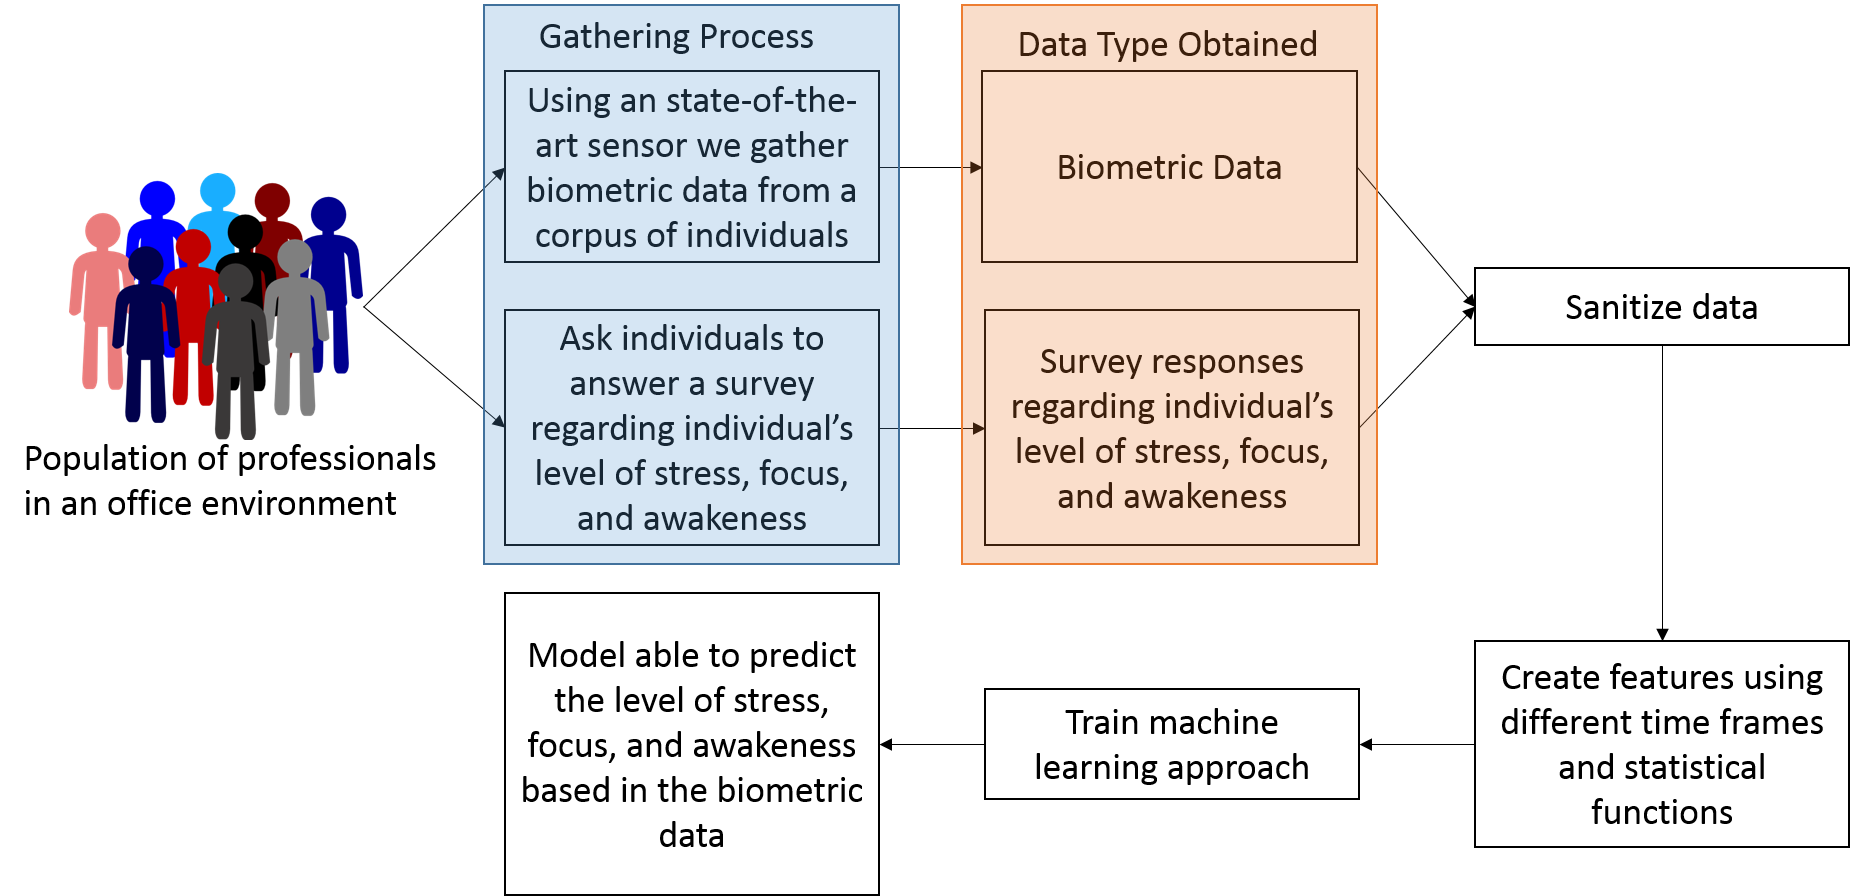
\includegraphics[width=0.5\textwidth]{Figure1.png}
%  \caption{Process used to gather data and create the machine learning model able to predict the level of stress, focus, and awakeness} 
%  \label{process}
%\end{figure}
%\todo{The figure or text in the boxes could be shortened a lot, maybe even just replaced with pictures of sensor and survey like question with 5point scale. At this point, i'm not sure the figure adds a lot.}

%Figure \ref{process} shows the overall process performed in this study. We started by selecting a population
%of professionals in an office environment.

We use state-of-the-art sensors to capture a stream of biometric data from each individual and a computer interaction tracker to collect computer interaction information during the time
of the study. 

The participants were asked to fill a survey 3 times a day: two during the working day, and
one at the end of the day, where they rated their level of stress, focus, and awakeness during
the day; and their level of stress, awakeness, productiveness, and overall feeling at the end of the day.
This was conducted over an eight week period, which is
400\% longer than previous studies~\cite{zuger18,Muller16}.

We then pick a set of time windows (10sec, 20sec, 30sec, 45sec, 1min, 2min, 3min, 5min, 7.5min, 10min, 20min, 30min, 45min, 1hour, 2hour, 3hour) to analyze. We applied different statistical measurements (mean, standard deviation, variance, median, percentile25, percentile75, interquartile range, maximum, minimum, range) to each of the collected biometric signals and the computer interaction data within the time windows selected. We then 
compared the performance of four different machine learning 
algorithms to be able to predict the survey responses based in the biometric and 
computer interaction data.

Based in the initial corpus of training data, we create a machine learning model that is able to accurately predict the responses for stress, focus, and awakeness for each of the individuals wearing the sensors.
We are therefore able to infer the answer within the spectrum to each of these indicators without the need to ask the participants to provide an answer.
\end{comment}

\subsection{Data Collection}

In this section we describe the two datasets that we collected from each study participant.

\subsubsection{Biometric Sensors}
Figure~\ref{everion} illustrates Biovotion's Everion, which we used to track the biometric signals of the study participants. The Everion is worn on the upper arm and provides continuous monitoring of certain biometric measurements.\footnote{https://biovotion.zendesk.com/hc/en-us/categories/201633909-Everion-Device} Previous studies~\cite{zuger18,sano2013stress,healey2005detecting,wijsman2011towards,zuger2015interruptibility,goyal2017intelligent} have used similar devices~\cite{Okada11,polar,fitbitCharge} to capture psycho-physiological and biometric measurements for shorter periods of time or capturing a smaller number of measurements.

\begin{figure}
  \centering
      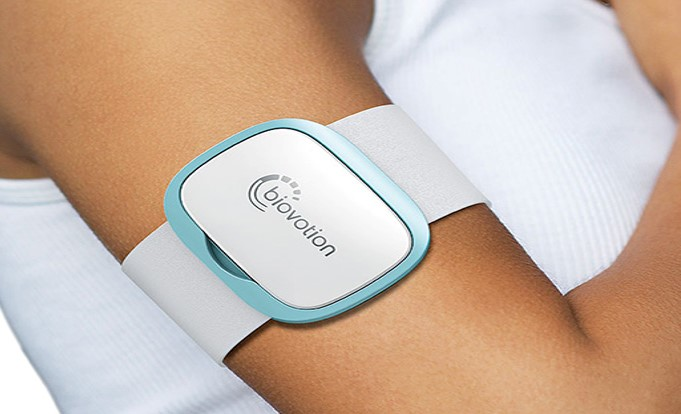
\includegraphics[width=0.4\textwidth]{Everion.jpg}
  \caption{We used Biovotion's Everion to collect biometric measurements from the participants}
   \label{everion}
\end{figure}

Table~\ref{signals} lists the biometrics measurements that we collected using the Everion. Each measurement is collected once per second, and each recorded observation has an associated timestamp and quality rating. Data collected by the Everion are uploaded to a server, from which we downloaded the data for use in our study.

\begin{table}[h!]
\begin{center}
%\small\addtolength{\tabcolsep}{-2pt}
\begin{tabular}{l l}
\hline
Biometric Measurement & Units of Measure \\ 
\hline
\textbf{Physical Activity} & \cite{fox1999,aldana1996}\\
\hspace{3mm}Intensity of motion & (No unit)  \\
\hspace{3mm}Energy Expenditure & Calories per second (cal/s)  \\
\hspace{3mm}Step counter & Steps  \\
\hline
\textbf{Heart} & \cite{haapalainen2010psycho,healey2005detecting,mulder1992measurement,haag2004emotion} \\
\hspace{3mm}Heart rate & Beats per Minute (bpm) \\
\hspace{3mm}Blood pulse wave & (No Unit)  \\
\hspace{3mm}Heart rate variability (RMSSD) & Milliseconds (ms) \\
\hspace{3mm}Blood oxygenation  & Percent (\%)  \\
\hspace{3mm}Blood perfusion & (No unit)  \\
\hline
\textbf{Skin} & \cite{healey2005detecting,haag2004emotion} \\
\hspace{3mm}Galvanic skin response &  kOhm  \\
\hspace{3mm}Skin temperature &  Degrees Celsius ($^{\circ}$C)  \\
\hline
\textbf{Respiration} & \cite{mulder1992measurement,healey2005detecting,haag2004emotion,masaoka1997}\\
\hspace{3mm}Respiratory rate & Breaths per Minute (bpm)  \\
\hline
%\textbf{Environmental}\\
%\hspace{3mm}Barometric pressure & Milibar (mbar)  \\
%\hline
\end{tabular}
\caption{Biometric measurements captured by the Everion, organized by category and with references to previous works using similar data}
\label{signals}
\end{center}
\vspace*{-4mm}
\end{table}



\subsubsection{Surveys}
\label{sec:Surveys}
Following guidelines from previous studies~\cite{Lalle16,Panwar18,Luo18} and 
following the preferrences of extensive user piloting, we sent via 
text message a survey request to each participant two times per 
work day. Pilot participants preferred these over other means, in part, due 
to them being accessible and noticeable anywhere in the office. 

We sent the 
first request at a random time between 9am and 11am 
and sent the second request at a random time between 1pm and 3pm. We 
randomized the request times to avoid either establishing or observing a 
standard behavioral pattern. That is, we did not want the participants to 
plan for the arrival of the survey request at a set time, and we did not 
want the survey request to overlap with a set daily behavior (e.g., coffee 
break every day at 2:30pm). Similarly, we avoided using tools which allow 
for too much freedom in response time~\cite{Adams18} since this would 
discurage participation in stressed timeframes and would bias the 
corpus. 
%This sentence was added in response to Reviewer 1 comment:
%There is already a lot of work on designing a new self-log, a self-report 
%tool which can blend into the workstation [1] or offers users more freedom 
%in time to self-report [2], or facilitate the self-log by using wearables.
The same survey was sent each time:
\begin{enumerate}
\item How awake are you right now?
\item How stressed do you feel right now?
\item How focused on work are you right now? 
\end{enumerate}
We used the phrase ``right now'' to capture each aspect in the moment (so as to permit later prediction of each aspect based on biometric data). The wordings of the questions are based on a previous survey of individuals in an organizational context~\cite{Gloor_etal:2010}. The use of awakeness (rather than sleepiness) in Question 1 is inspired by previous work~\cite{Wilhelm_Schoebi:2007} and to some extent also captures the ``arousal'' aspect of the affective space~\cite{Russell:1980}.


%\todo{we are not using the last survey for anything in this paper, so I'd leave it out}
%One last survey was sent at the end of the day, at 4:25pm which asked the 
%four different questions
%detailed below:
%\begin{itemize}
%\item How awake have you been today?
%\item How stressed did you feel today?
%\item How productive have you been today?
%\item How do you feel about your work day?
%\end{itemize}

Following guidelines from similar previous studies~\cite{fogarty05,tanaka11}, we asked the participants to respond to each question using a 5-point Likert scale ranging from 1 (not at all awake/stressed/focused) to 5 (extremely awake/stressed/focused). Each participant response, as stored by Survey Gizmo, comprised the date, the time at which the response was initiated, the time at which the survey was submitted, the unique identifier for the participant, and the responses submitted by the participant.

%!TEX root = bioPrediction_main.tex

\subsection{Data Preparation}

In this section we describe how we preprocessed the collected data for use in training and testing machine learning models.

\subsubsection{Data Linking}

We linked the collected biometric data and survey responses for each participant. Linking the data is necessary to construct training and test datasets for use in creating and evaluation machine learning models.

Our linking approach is as follows. From the start time of each survey response, we look back one hour for available biometric data. For each minute in that hour-long time window, we check for biometric data to associate with the survey response. For example, if a participant started a survey response at 11:05am, we look for biometric data in the time frame 10:05am to 11:05am. If biometric data is available in the hour-long time window, we consider the survey response to have associated biometric data. Otherwise, we exclude the survey response from our dataset.

Reasons for a survey response to lack associated biometric data include:
\begin{itemize}
\item The participant not wearing the Everion in the hour before before beginning the survey
\item The Everion not recording data in the hour before the participant began the survey (e.g., due to low battery)
\item Biometric data not being uploaded successfully to the server
%\item Compatibility issues between the sensor and the OS tracking the participant's data
%\item Issues accessing the data uploaded by the participants
\end{itemize}

Figure~\ref{surveyBio} illustrates the number of survey responses with associated biometric data for each study participant. Participant S2 and S12 have particularly low numbers of usable survey responses. In each of these cases, the issue related to biometric data not being uploaded successfully to the server.

\begin{figure}
  \centering
      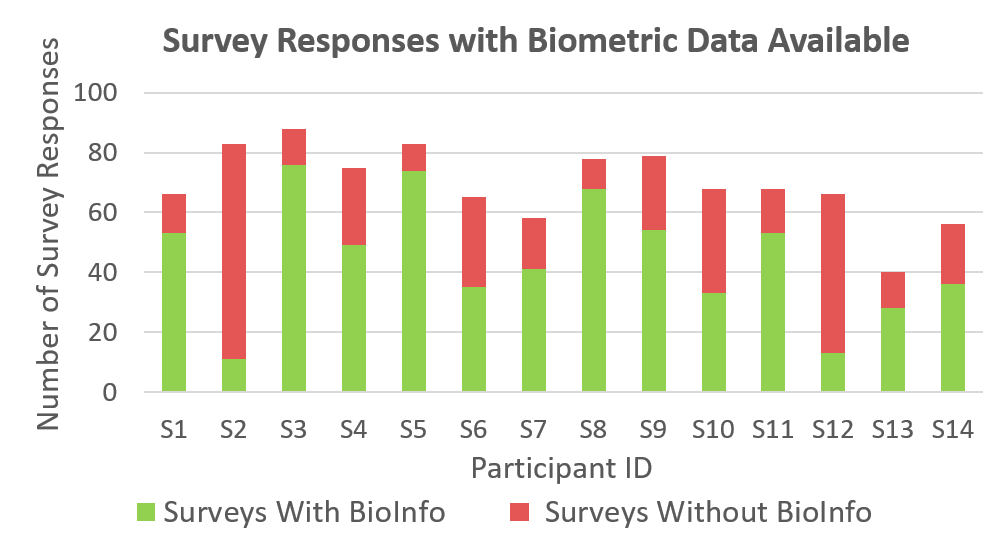
\includegraphics[width=0.5\textwidth]{DuringTheDay.png}
  \caption{The figure shows the biometric data available per each participant. Green sections represent survey responses with biometric
  data available, red sections responses with no biometric data available}
   \label{surveyBio}
   \vspace*{-4mm}
\end{figure}


\subsubsection{Feature Extraction}
We extracted features from the biometric data to provide as input to machine learning models. Previous studies~ \cite{vorburger05,zuger2015interruptibility} identify time windows as an important factor that impacts the prediction accuracy of a classifier. We considered many time windows from the literature on biometric analysis~\cite{zuger18}, ranging from 10 seconds to 3 hours. Specifically, we considered the following time windows: \textit{10sec, 20sec, 30sec, 45sec, 1min, 2min, 3min, 5min, 7.5min, 10min, 20min, 30min, 45min, 1hour, 2hour, 3hour}.

From the start time of each survey response, we look back the amount of time that corresponds to each time window, and we create features for all of the biometric data available in that time window. For example, if a participant started a survey response at 11:05am, for the 30min time window, we create features using all of the available biometric data from 10:35am to 11:05am. For each time window, we calculate 10 statistical measurements from the biometric data to create 10 distinct features. Specifically, the 10 statistical measurements are: mean, standard deviation, variance, median, percentile25, percentile75, interquartile range, maximum, minimum, and range. Thus, for each survey response, we generate a large number of corresponding features based on three factors: biometric measurement, time window, and statistical measurement. In addition to these biometric features, we also considered the time of day in which the questions were asked.

\subsubsection{Response Transformations}
Table~\ref{responseDistribution} illustrates the distribution of responses from each participant for each of the three survey questions (which are listed in Section~\ref{sec:Surveys}). The figure shows that there is a notable imbalance in the distribution of the self-reported responses provided by the participants. Most participants did not use all five points of the five-point Likert scale in their responses, and the distributions tend to skew toward one side or the other, depending on the question. Thus, we binarized the survey data into a two-point scale to give the machine learning models the best possible chance to make useful predictions. The two points in the binary scale represent negative or positive responses for each of the three human aspects of interests (e.g., not stressed or stressed). 

We binarized the survey responses as follows. For each participant, we calculated the median response value for each question. We classified each response below the median as 0 ('negative') and each response above the median as 1 ('positive'). The distribution for the stress question skewed left, so we included the median values in the 'positive' class, while the distributions for focus and awakeness skewed right, so we included those median values in the 'negative' class.

\subsubsection{Oversampling}
Even after binarizing the responses as described in the previous section, we found the distribution of responses was still quite imbalanced for many of our participants. This can be seen in the distribution columns in Table \ref{tab:accuracy}. To combat this, we applied random oversampling to our training sets, which artificially rebalances the dataset by creating randomly replicated data in the minority class. This has been a commonly used technique in previous studies on unbalanced datasets \cite{chawla2004,yap2014}.


\begin{table}
  \centering
      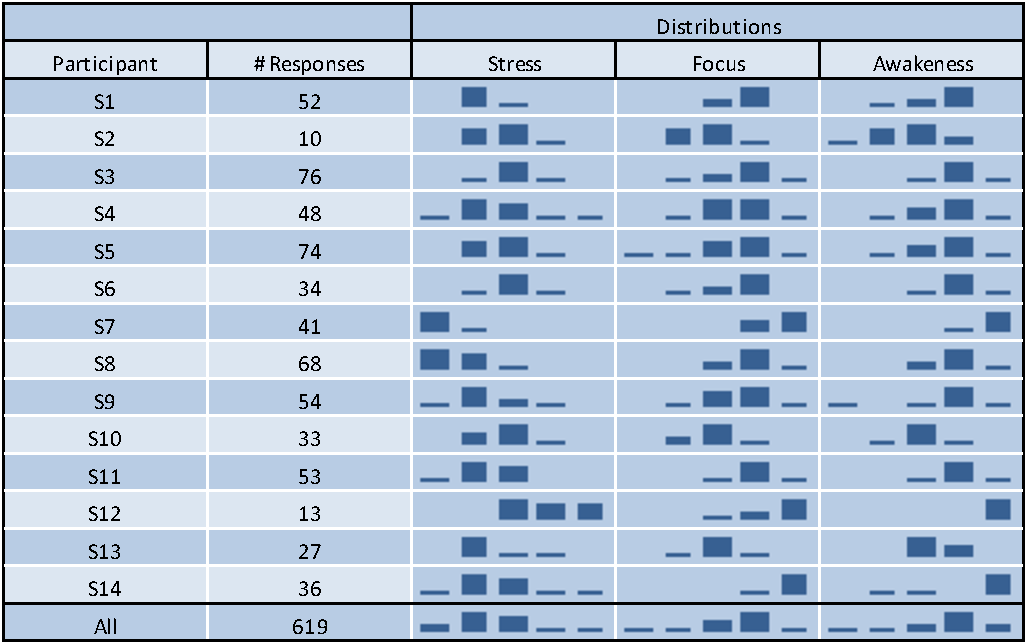
\includegraphics[width=0.5\textwidth]{distributiontable.pdf}
  \caption{The distribution of the responses of each participant to the three questions asked during the day are shown. Each bar in the histograms represent one of the 5 values on the 5-point Likert scale we asked participants to respond with, where the far left side of the histograms are 1/Not at all, and the far right sides are 5/Extremely}
   \label{responseDistribution}
   \vspace*{-9mm}
\end{table}


%!TEX root = bioPrediction_main.tex
%%!TEX root = bioPrediction_main.tex
%%!TEX root = bioPrediction_main.tex
%\input{bp_results_1}
%%\input{bp_results_2}

%\section{Analysis and Results}

%% To evaluate the efficacy of continuously predicting a knowledge worker's stress, focus, and awakeness in the workplace, we trained and tested machine learning classifiers using a leave-one-out cross validation. For prediction, we used the features extracted from the collected data as the input data, and binarized the participants' self-reported responses on stress, focus, and awakeness into two classes each (e.g., 'stressed' and 'not stressed') to use as output measures.

\section{Observed Trends Over Time in Stress and Awakeness Levels}
\label{stressTrends}

To gain insights into how knowledge workers experience stress and awakeness over an
extended period of work, we examined the end of day survey responses
collected from each participant to see if any identifiable trends
emerged. As we noted in the last section, we did not ask
participants about focus in the end of  day surveys as focus is an 
aspect relevant at a particular moment in time rather than an aspect
for an extended period of work. We used data from 13 of the 14 participants - we excluded one participant
from this analysis as they experienced atypical stress
levels in the latter half of the study due to factors outside of our
control.

\subsection{Stress Levels}
Overall, we identified three prominent characteristics in the stress levels.
%\rev{We describe characteristics noted in the reporting of the knowledge workers about the stress they experienced over the duration of the study.}

\begin{figure}[h!]
  \centering
      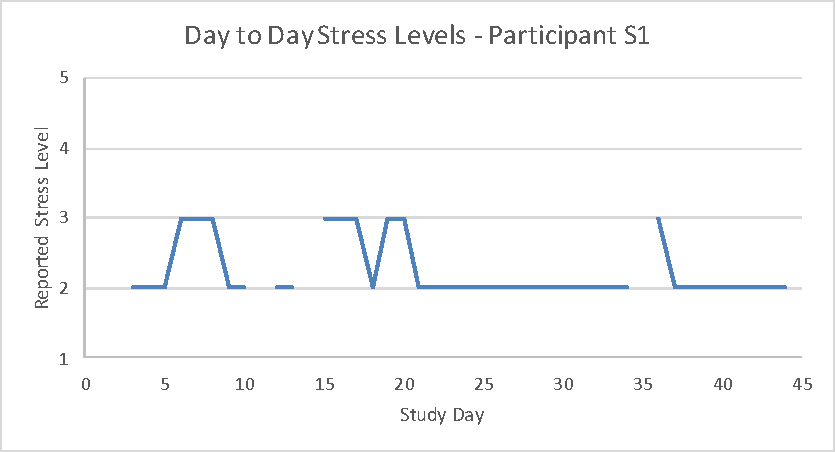
\includegraphics[width=0.7\textwidth]{s1_stress.pdf}
      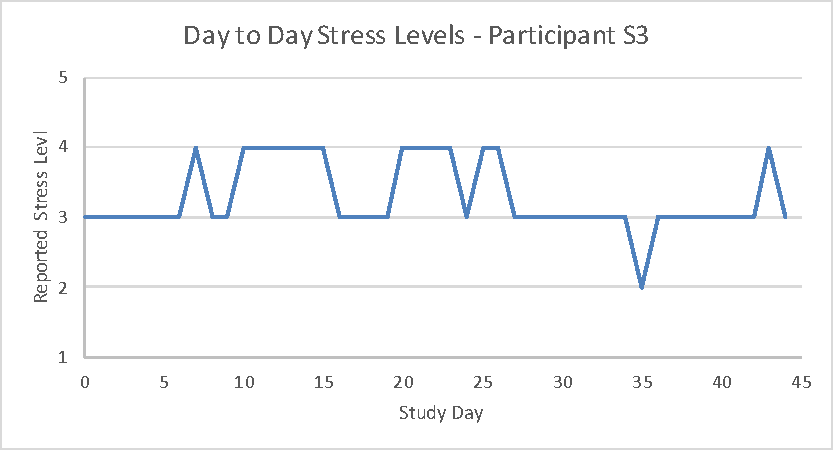
\includegraphics[width=0.7\textwidth]{s3_stress.pdf}
  \caption{The day-to-day stress levels reported by two participants (S1 and S3) are shown. The y-axis represents values on the 5-point Likert scale we asked participants to respond with ranging from 1/Not at all stressed to 5/Extremely stressed. The x-axis represents the day of the study on which the value was recorded (from 0-45). Some gaps are present in the chart for S1 as they did not report their stress level on those days.}
   \vspace*{-2mm}
   \label{fig:dailyStress}
\end{figure}


\subsubsection{Baseline Stress Levels}
%\noindent\textit{\textbf{Baseline Stress Levels.}}
Common amongst all participants was a trend to select one stress rating
far more frequently than any other. We will refer to this value as the
participant's baseline stress level. All but one participant reported
their perceived stress level for the day as their baseline stress
level more than 50\% of the time. In total, the baseline values made
up 65\% of the reported values collected from
participants. Interestingly, while participants sometimes saw periods
of sustained increases in stress, lasting as many as 6 consecutive
workdays in the most extreme case, participants would always return to
their baseline stress level at some point.


The baseline stress level varied significantly between participants. \rev{Seven}
participants (54\%) reported feeling average stress levels most frequently
(rating 3 on our scale), while \rev{five} (38\%) reported feeling little stress
(rating 2) and \rev{one} (8\%) reported feeling no stress at all (rating 1). Figure \ref{fig:dailyStress} illustrates these points using  data from two participants, showing the tendency to report and return to baseline stress levels, as well
as a distinct difference in baseline stress level (rating 2 for S1 vs rating 3 for S3). Gaps in the chart for S1 represent days for which the participant did not report their stress level.


\subsubsection{Stressful Days Tend to Cluster}
Accounting for the variance between participants perceived stress
baselines, we consider a stressful day to be one that represents a
deviation of \rev{one} or more stress levels above the participant's
baseline. Of the 93 stressful days we observed in total, we found that
39 (41\%) of these days occurred in groupings of two or more
consecutive stressful workdays. The most common size of these groups
was two workdays, while the largest group we observed was six
workdays.  The day after a stressful day is much more likely to be a
stressful day as compared to any other day with a 0.55 average increase
over baseline, compared to 0.02 average increase over baseline.

\subsubsection{Extreme Changes in Stress Levels are Rare}
After accounting for each participant's perceived stress baseline, we
examined the frequency of deviations from the baseline. We found that
participants were far more likely to report a stress level that was
within \rev{one} point of their baseline, than to report a stress level 2 or
more points away. These extreme deviations represented only 15\% of
all reported values, which differed from the \rev{participant's} baseline. As
well, the majority (78\%) of these deviations came from just two
participants. This suggests that some people may be less resilient to
the stress of the workplace than others. For most participants,
extremely stressful days were few and far between.

\subsection{Awakeness}
We applied the same analyses described above to the \rev{self-reported} awakeness levels of our participants. Compared with the reported stress levels, we observed the same trend of participants reporting one baseline far more commonly than any other. We did not find there to be a significant correlation between reported stress and awakeness levels. Overall, \rev{participant's} awakeness levels fluctuated significantly less than their stress levels (73.1\% of reports were at the baseline level, compared to 65.1\% for stress, p < 0.05). Participants were unlikely to experience days with heightened (above baseline) awakeness. Such days made up only 6.0\% of the total observed \rev{workdays} across all participant. Most of these days came from one participant, S2, who reported 15 heightened awakeness days compared to the next highest, S13 with four. Large deviations (>1 point deviation) from each participants baseline awakeness levels were extremely uncommon, accounting for only \rev{nine} (2.1\%) of our total observations. Similarly to what we observed with high stress days, low awakeness days frequently came in clusters of two or three days in a row. Given that the immediately preceding day was a low awakeness day\rev{;} a given day was 228.2\% more likely to be a low awakeness day than when considering any day at random (p < 0.0001).


\begin{table}[]
    \centering
\rev{\begin{tabularx}{\textwidth}{|c|c c c|c c c|}
    \hline
        &
        \multicolumn{3}{c|}{Stress} & 
        \multicolumn{3}{c|}{Awakeness} \\
        \hline
        \textbf{Variable} & \centering
        \textbf{\rev{F.E.E.}}& \textbf{p-value} & \textbf{\rev{C.I. (95\%)}} & \centering \textbf{\rev{F.E.E.}}  & \textbf{p-value} & \textbf{\rev{C.I. (95\%)}}\\
        \hline
        Monday & \centering -0.033 & 0.745 & \rev{$(-0.234, 0.167)$} & \centering -0.058 & 0.497 & \rev{$(-0.227, 0.110)$}\\
        Tuesday & \centering 0.028 & 0.773 & \rev{$(-0.164, 0.221)$} & \centering 0.036 & 0.662 & \rev{$(-0.126, 0.198)$}\\
        Wednesday & \centering 0.163 & 0.100 & \rev{$(-0.031, 0.357)$} & \centering -0.018 & 0.830 & \rev{$(-0.181, 0.145)$}\\
        Thursday & \centering 0.022 & 0.821 & \rev{$(-0.169, 0.213)$} & \centering 0.076 & 0.927 & \rev{$(-0.085, 0.238)$}\\
        Friday & \centering 0.082 & 0.473 & \rev{$(-0.142, 0.306)$} & \centering -0.178 & 0.025 & \rev{$(-0.334, -0.022)$}\\
        Month End & \centering 0.044 & 0.687 & \rev{$(-0.171, 0.259)$} & \centering -0.082 & 0.374 & \rev{$(-0.263, 0.099)$}\\
        \hline
    \end{tabularx}
    \caption{\rev{Fixed effects estimates (F.E.E.), 95\% confidence intervals and associated p-values for the explanatory variables (day of week and proximity to month end) that we examined in our linear mixed model analysis.}}    \label{tab:mixedModel}}
\end{table}





\subsection{Explaining Fluctuations}
In an attempt to explain some of the fluctuations in stress and awakeness that our participants were experiencing, we created a linear mixed model with the self-reported daily stress and awakeness levels as dependent variables and the participants as random effects. We experimented with day of the week and proximity to beginning or end of month as possible explanatory variables. Ultimately, the analysis showed that none of the variables that we examined had a significant explanatory power with respect to our participants perceived stress levels.
For awakeness, we found  that there was a small (\rev{fixed effects estimate}: -0.178) yet significant decrease in awakeness levels on Fridays in particular. Table \ref{tab:mixedModel} shows some of the detailed results of these analyses. These results show the difficulty of explaining a person's stress and awakeness via simple measures, and point to the need for additional instrumentation and data collection if we are to successfully understand and make predictions about these human aspects in the workplace.




\section{Predicting Stress, Focus and Awakeness in the Moment}
% random forest best
\label{secOverallAccuracy}

To investigate whether stress, focus and awakeness can be predicted in
the moment based on biometric measures,
we investigated classifiers trained
for each individual and across all participants. We report on the effectiveness of
these classifiers and the features that are important in predicting stress, focus
and awakeness.

\subsection{Data Preparation}

\rev{In a machine learning context, data preparation and utilization is an essential part of the proposed solution. To prepare} the collected data for use in training and testing \rev{our proposed} machine learning models, we performed \rev{the following} steps.


\subsubsection{Data Cleaning}
All data recorded by the Everion is associated with a quality score ranging from 0-1 that is calculated using proprietary methods. In accordance with the recommendations of Biovotion,
to prevent our results from being effected by erroneous data we set a quality threshold of 0.5 and discarded any data gathered which had a quality rating below this threshold. 

\subsubsection{Data Linking}

We linked the collected biometric data and survey responses for each participant. Linking the data is necessary to construct training and test datasets for use in creating and evaluating machine learning models.

To link the data, we look back one hour from the start time of each survey response for
available biometric data.  For example, if a participant started a survey response at 11:05am, we look for biometric data from between 10:05am to 11:05am. If no biometric data was recorded in the hour time window, we exclude the survey response from the dataset. Otherwise, we consider the survey response to have associated biometric data.

There are several reasons for a survey response to lack associated biometric data:
\begin{itemize}
\item The participant was not wearing the Everion in the hour before beginning the survey.
\item The Everion was not recording data in the hour before the participant began the survey (e.g., due to low battery).
\item Biometric data was not being uploaded successfully to the server.
%\item Compatibility issues between the sensor and the OS tracking the participant's data
%\item Issues accessing the data uploaded by the participants
\end{itemize}

Figure~\ref{surveyBio} illustrates the number of survey responses with associated biometric data for each study participant. 
%This was added to address REviewer 2's concern: Is it correct that the maximum number of responses should have been 112 on the surveys?
The total number of responses per participant is affected by their response rate and by the number days out-of-office (e.g., vacations, holidays, etc.). 
Participant S2 and S12 have particularly low numbers of usable survey responses. In each of these cases, the issue related to biometric data not being uploaded successfully to the server.

\begin{figure}
  \centering
      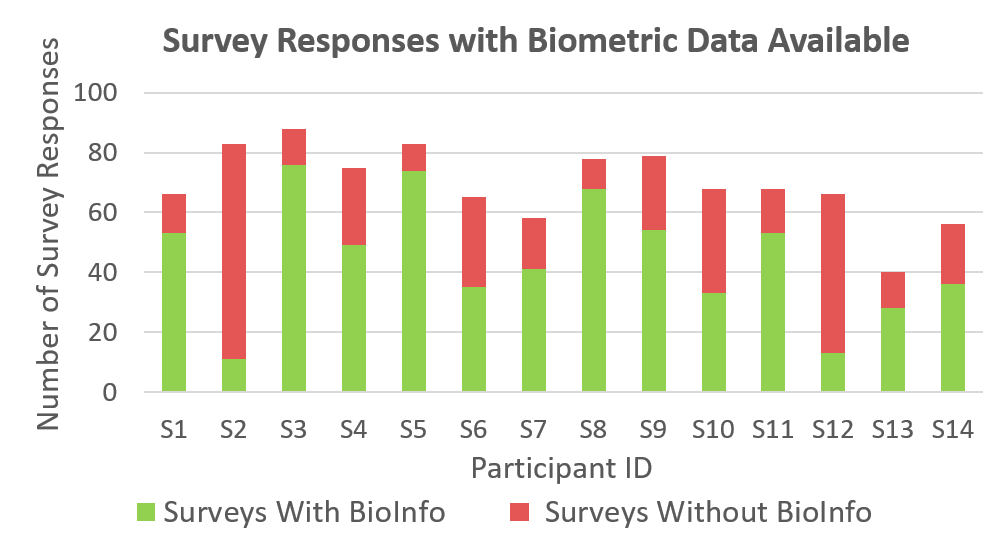
\includegraphics[width=0.8\textwidth]{DuringTheDay.png}
  \caption{The figure shows the biometric data available per each participant. Green sections represent survey responses with biometric
  data available, red sections responses with no biometric data available}
   \label{surveyBio}
   \vspace*{-4mm}
\end{figure}


\subsubsection{Feature Extraction}
We extracted features from the biometric data to provide as input to machine 
learning models. Previous 
studies~ \cite{vorburger05,zuger2015interruptibility} identify time windows as an 
important factor that impacts the prediction accuracy of a classifier. We 
considered many time windows from the literature on biometric 
analysis~\cite{zuger18}, ranging from 10 seconds to 3 hours. Specifically, we 
considered the following time windows: \textit{10sec, 20sec, 30sec, 45sec, 
1min, 2min, 3min, 5min, 7.5min, 10min, 20min, 30min, 45min, 1hour, 2hour, 
3hour}.

From the start time of each survey response, we look back the amount of time 
that corresponds to each time window and we create features for all of the 
biometric data available in that time window. For example, if a participant 
started a survey response at 11:05am, for the 30min time window, we create 
features using all of the available biometric data from 10:35am to 11:05am. 
If there is a large portion ($\geq$50\%) of data missing (either because of a recording issue or because of low quality data) from the time window considered, then the time window is marked as missing. In this case, features are imputed based on the mean of other samples of the same feature for that participant. This is an effective and commonly used technique, which is preferable to the alternative of deletion as it preserves our already small sample size~\cite{hawthorne2005imputing}.
For each time window, we calculate 10 statistical measurements from the 
biometric data to create 10 distinct features. Specifically, the 10 
statistical measurements are: mean, standard deviation, variance, median, 
25\textsuperscript{th} percentile, 75\textsuperscript{th} percentile, interquartile range, maximum, minimum, and 
range. Thus, for each survey response, we generate a large number of 
corresponding features based on three factors: biometric measurement, time 
window, and statistical measurement. In addition to these biometric 
features, we also considered the time of day in which the questions were 
asked. These features are created to predict the responses described by the 
ground truth. To attempt to account for inter-participant differences, we normalized all features on a per-participant basis.

\begin{table}
  \centering
      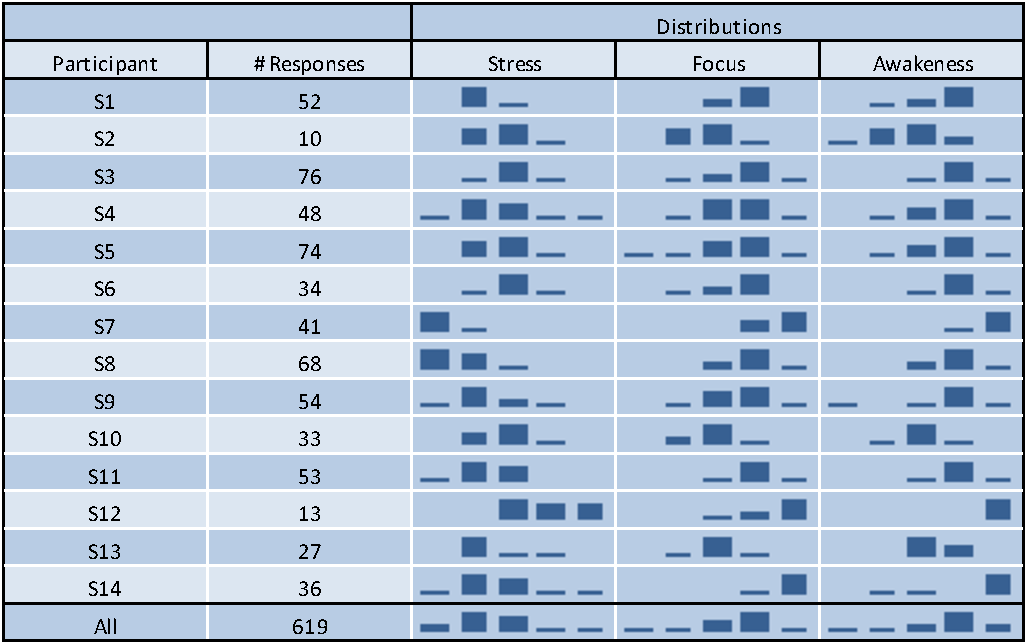
\includegraphics[width=0.8\textwidth]{distributiontable.pdf}
  \caption{The distribution of the responses of each participant to the three questions asked during the day are shown. Each bar in the histograms represent one of the \ref{five} values on the 5-point Likert scale we asked participants to respond with, where the far left side of the histograms are 1/Not at all, and the far right sides are 5/Extremely}
   \label{responseDistribution}
   %\vspace*{-2mm}
\end{table}

\subsubsection{Response Transformations}
Table~\ref{responseDistribution} illustrates the distribution of responses from each participant for each of the three survey questions (listed in Section~\ref{sec:Surveys}). The figure shows that there is a notable imbalance in the distribution of the self-reported responses provided by the participants. Most participants did not use all five points of the five-point Likert scale in their responses, and the distributions tend to skew toward one side or the other, depending on the question. Given 
this distribution and based on our earlier observation that the participants tended to adhere to a baseline reporting level for stress and awakeness, we elected to simplify the problem from \rev{five} classes to \rev{two}. This transformation enables us to more easily represent patterns in the data, such as when a participant fluctuates from a normal to high stress level. To perform this transformation, \rev{we began by calculating the median response value for each participant and each question}. We classified each response below the median as 0 (`negative') and each response above the median as 1 (`positive'). The distribution for the stress question skewed left, so we included the median values in the `positive' class (i.e. `stressed'), while the distributions for focus and awakeness skewed right, so we included those median values in the `negative' class (i.e. `not focused', `not awake').

With this method, we transformed the survey data into a two-point scale, representing  negative or positive responses for each of the three human aspects of interests (e.g., not stressed or stressed). 

\subsubsection{Oversampling}
Even after binarizing the responses as described in the previous section, we found the distribution of responses was still quite imbalanced for many of our participants. This can be seen in the distribution columns in Table \ref{tab:accuracy}. To mitigate this effect, we applied random oversampling to our training sets, which artificially rebalances the dataset by creating randomly replicated data in the minority class. This technique has commonly been used  in previous studies on unbalanced datasets \cite{chawla2004,yap2014}.

\begin{comment}
\begin{table}[h]
	\begin{centering}
	\small\addtolength{\tabcolsep}{-1pt}
    \begin{tabular}{llll}
      \hline
      Variable & K & \# Estimators & Minimum Samples Split \\
      \hline
      Stress & 300 & 100 & 4\\
      Focus & 200 & 50 & 4\\
      Awakeness & 800 & 100 & 4\\
      \hline
    \end{tabular}
    \caption{The hyperparameters selected by grid search analysis to tune our random forest models. K refers to the number of features selected.}    \label{tab:hyperparams}
    \end{centering}
\end{table}
\end{comment}


\subsection{Selecting a Classifier Algorithm}

\rev{Many different algorithms can be used to build a classifier.} To select an
algorithm, we compared multiple classifiers using the popular machine learning library scikit-learn~\cite{pedregosa11},  evaluating each one by using leave-one-out cross validation. Our analysis showed that random forest outperforms all other classifiers, including Na\"ive Bayes, decision trees, support vector machine, and a multilayer perceptron neural network. For the remainder of this paper, we refer to a random forest classifier.%\\[-0.1cm]
% for stress they were (minimum samples for split = 4, # of estimators = 100, max features = 0.5, k=300), for focus they were (minimum samples for split = 4, # of estimators = 50, max features = 0.5, k=200), and for awakeness they were (minimum samples for split = 4, # of estimators = 100, max features = 0.25, k=800)



\begin{table*}[h]
  \centering
  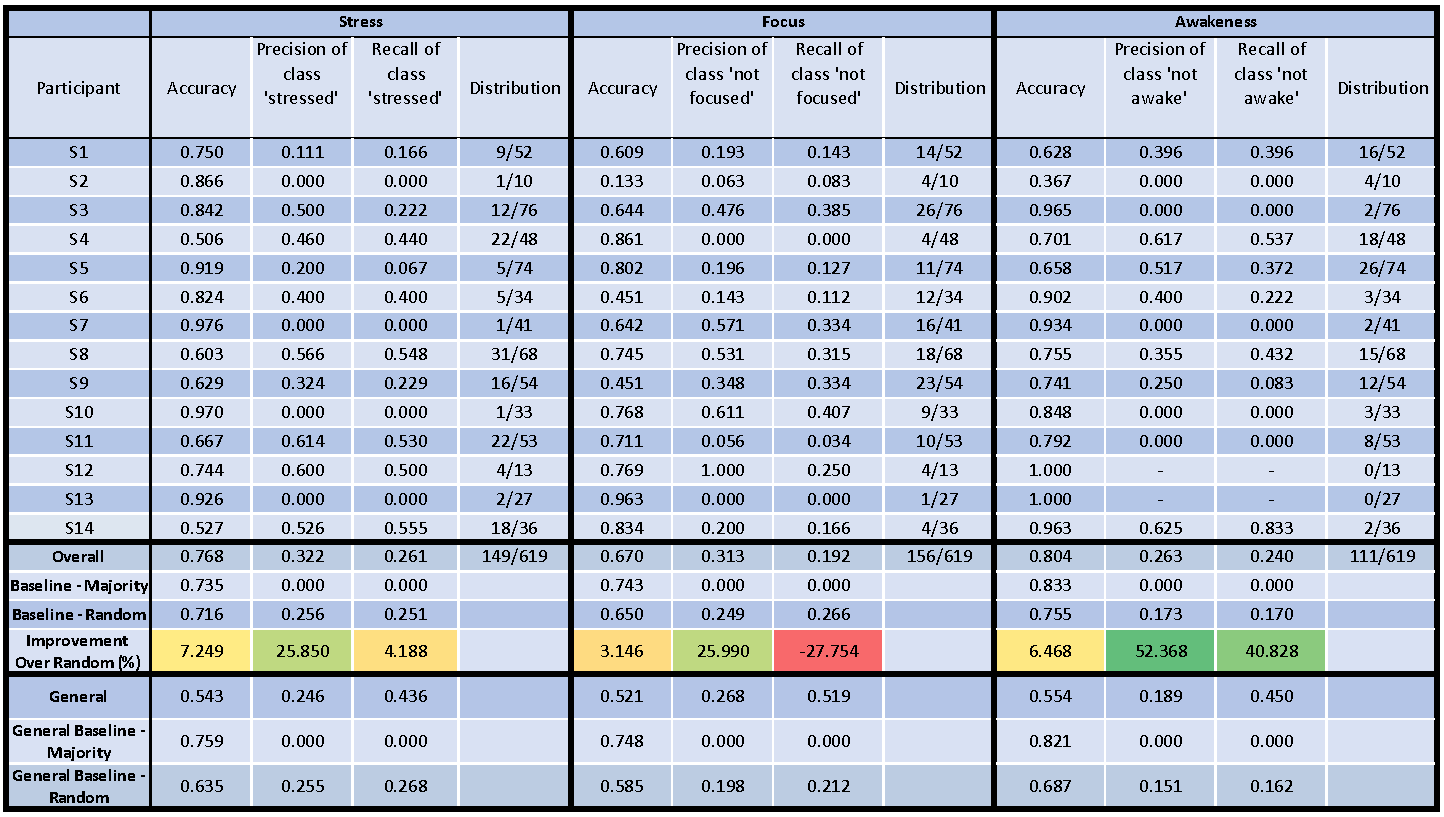
\includegraphics[width=1.0\textwidth]{rq1performance_v2.pdf}
  \caption{Results of predictions using the individual models. The distribution columns show the proportion of the minority class out of the total number of responses for each of the three variables. The baseline rows represents the averaged results of our baseline classifiers. The general row shows the averaged results of our models trained on all participants.}\label{tab:accuracy}%\todo{revise caption}}
  \vspace*{-4mm}
\end{table*}

\subsection{Individual Classifiers}
%\noindent\textit{Results of Individual Classifiers}\\
Since peoples' experience of stress, focus, and awakeness (as well as
their physiological manifestations) can vary substantially
(e.g.,~\cite{Hernandez11}), we first trained and evaluated individual classifiers
for each participant (as opposed to a general one for all
participants) using leave-one-out cross validation. The results of our analysis are reported in
Table~\ref{tab:accuracy}. For our analysis, we report values of
accuracy, one of the most commonly used metric to compare performance,
as well as precision and recall of the classes of interest:
`stressed', `not focused', and `not awake'. Since the imbalance in the
data can lead to high accuracy values if a classifier always just
predicts the most likely/frequent class while ignoring the class of
higher importance and interest, precision and recall of the class of
interest are also important to
consider~\cite{yap2014,bhattacharyya_data_2011,Hernandez11}.

\rev{Besides} our results, for the purposes of comparison\rev{,} we also present two commonly used baselines in this table - a majority classifier, which always predicts the larger of the two classes considered, and a stratified random classifier which randomly chooses between the two classes, but with a proportional bias towards the larger class.

For some users (i.e., S1. as seen in Table \ref{responseDistribution}), the imbalance in their data was so extreme that even after adjusting by oversampling\rev{, we were not able} to create a reasonable classifier. These scenarios are difficult to predict\rev{,} as any classifier will not have enough variance in its training data for the 'stressed' situation to adequately distinguish it from the non-stressed case.


% However, the imbalance in the data can lead to a classifier with high accuracy if it always just predicts the more likely class while ignoring the class of higher importance and interest in our case (i.e. stressed, not focused, not awake). Therefore, we further report the precision and recall for the three classes 'stressed', 'not focused' and 'not awake'. 


Overall, we were able to use extracted physiological features to
predict all three aspects with reasonable accuracy, precision, and
recall. We present a comparison between the averaged results of our individual classifiers and those of the baseline stratified random \rev{classifier} in the ``Improvement Over Random'' row of Table \ref{tab:accuracy}. This is calculated as the difference between the overall average and the baseline results, divided by the baseline results (for example, $\frac{Acc_{Overall} - Acc_{Random}}{Acc_{Random}}$). We do not compare our results with the majority classifier directly as this classifier achieved precision and recall scores of zero when predicting stress, lack of focus, and lack of awakeness, making a meaningful comparison \rev{unfeasible}. The improvement percentages demonstrate that the predictions made by our classifiers are much better than random after correcting for the imbalance in our dataset.

While the individually trained classifiers
improved on average across all participants upon the baseline in all
cases except in recall of `not focused', the improvement was
substantially higher for awakeness (52.4\% improvement in precision,
40.8\% in recall, and 6.5\% in accuracy) than for stress or focus. In addition,
the performance of the individually trained classifiers varied greatly
across participants. While some participants showed a large
improvement, for others the baseline performed much better than the
individually trained classifier. For instance, for predicting
`stressed', the individual classifiers improved upon the baseline for
S4, S6, S8, S11, S12, and S14 with a maximum improvement of 152.0\% in
precision and 111.1\% in recall for S12, while they did worse for S1,
S3, S5, S7, S9, S10, and S13, and in the worst cases did not correctly
predict a single instance of `stressed'. Typically, users that have the
lowest precision and recall values are those where the data is the
most imbalanced.\\[-0.1cm]
% We attribute these discrepancies to the large differences in response distributions between participants, as well as to the subjectivity of self-reporting.
%
%(improvement: 8\% precision, 1\% recall, 8\% accuracy), the individual performance varied greatly among participants. Some participants showed negligible difference in comparison to the baseline classifier, e.g. subject ..., while others showed a large improvement, e.g. subject ...
%\begin{table}[h!]
%\begin{centering}
%\begin{tabular}{lll}
%\hline
%Participant & Recall Improvement (\%) & Precision Improvement (\%)\\
%\hline
%S12 & 184.6 & 88.4 \\
%S6 & 66.7 & 85.8 \\
%S11 & 50.0 & 44.4 \\
%S8 & 32.4 & 26.7 \\
%S14 & 14.7 & 9.8 \\
%S4 & 5.6 & 5.5 \\
%S9 & -55.4 & -46.8 \\
%S3 & -90.0 & -82.1 \\
%S1 & -100.0 & -100.0 \\
%S5 & -100.0 & -100.0 \\
%S7 & -100.0 & -100.0 \\
%S10 & -100.0 & -100.0 \\
%S13 & -100.0 & -100.0\\
%S2 & - & -\\
%\hline
%\end{tabular}
%\caption{Percentage improvement in recall and precision for stress, using our approach compared to the baseline, on an individual level. For participant 2, the baseline achieved a precision and recall of 0, thus the improvement is undefined}
%\end{centering}
%\label{tab:indImprovement}
%\end{table}


\subsection{Feature Selection and Importance}
%\noindent\textit{Feature Selection and Importance}\\
There are a large variety of features that can be (and have been) calculated in previous research for each of the basic measurements listed in Table~\ref{signals}, such as the mean, standard deviation, maximum, and interquartile range. In addition, each of these metrics can be combined with the various time windows captured of a basic measurement, resulting in a large feature space. To reduce the feature space, we experimented with multiple feature selection methods, including selecting the top k highest correlated features by various metrics such as mutual information, Pearson's correlation coefficient, ANOVA's F-value, as well as wrapper methods such as recursive feature elimination, optimizing mean decrease accuracy by iteratively permuting features, and only selecting features that exceed a certain Gini importance threshold. We found that all methods produced similar results with respect to accuracy, precision, and recall for the individual models. Ultimately, we elected not to utilize any feature selection in order to simplify our approach, as we found there to be minimal differences in performance between the techniques, and the random forest algorithm is capable of (and robust for) handling datasets with many features.

%Respiration rate is also highly important for stress (#3 , 14.4%) but I'm not sure what previous works say about correlation with stress
Overall, the features that were selected as the important ones for the individual models based on the random forest algorithm varied greatly across participants. Yet, some feature categories were considered to be important more frequently than others. Table~\ref{tab:featureImportance} shows the averaged Gini importance for the feature categories used for predicting stress. Heart rate variability proved to be an important measure for all of the aspects of interest, ranking as the most important feature category for both stress and awakeness, and the second most important one for focus. This is not surprising, as heart rate variability and skin temperature have been shown in several previous studies to be possible indicators for stress levels~\cite{dishman2000stress,mcduff16,kataoka00}. We also found blood pulse wave to be an important indicator for both focus and awakeness, but less important for stress, while respiration rate was important in stress and focus but not awakeness. Besides these mentioned feature categories, there was great variation in which measures were important to which of the three aspects. This shows that there is a clear benefit to having multiple biometric streams available for predicting stress, focus and awakeness.\\[-0.1cm]


\begin{table}[h!]
  \begin{centering}
  \begin{tabular}{llll}
    \hline
    Feature Category & Stress & Focus & Awakeness\\
    \hline
    Heart Rate Variability & 18.3\% & 13\% & 13.6\%\\
    Blood Pulse Wave & 10\% & 14.2\% & 13.1\%\\
    Heart Rate & 8.7\% & 12.6\% & 10.3\%\\
    Skin Temperature & 15.7\% & 9.8\% & 10\%\\
    Galvanic Skin Response & 6.6\% & 8.2\% & 5.1\%\\
    Respiration Rate & 14.8\% & 12.7\% & 10\%\\
    Oxygen Saturation & 5.6\% & 4.3\% & 2\%\\ 
    Energy Expenditure & 6\% & 7.7\% & 4.8\%\\
    Activity & 4.6\% & 7.8\% & 7.6\%\\
    Steps & 1.7\% & 0.8\% & 0.9\%\\
    Time of Day & 0\% & 0.1\% & 0.5\%\\
    \hline
  \end{tabular}
  \caption{The averaged Gini importance of each feature category, per response variable.}
  \label{tab:featureImportance}
  \end{centering}
  \vspace*{-2mm}
\end{table}

\subsection{Individual vs.\ General Model}
%\noindent\textit{Individual vs.\ General Model}\\
Individual models are trained specifically for each individual and thus require a data collection period before they are capable of making accurate predictions. On the other hand, the idea of general models is to be able to train them on already collected data and then  to be able to apply them even to new and unseen individuals, thus overcoming the cold-start problem. Given the large individual differences in biometrics, training a general model to achieve an adequate accuracy for new individuals is not necessarily possible. 

To examine the performance of a general model for our participants, we trained three general models, one for focus, one for awakeness and one for stress. We roughly followed the same procedure as for the individual models. Due to the larger amount of data available in the general case, we used the more common random undersampling, which randomly selects elements in the majority class to exclude from the dataset, instead of random oversampling to balance the distribution of the dataset. The models were trained on the datasets of 13 of the 14 participants, and then evaluated on the dataset of the last (leave-one-participant-out cross-validation), repeating this process for all 14 participants. 

The bottom \rev{three} rows of Table \ref{tab:accuracy} present the averaged performance results for this approach in terms of accuracy, precision, and recall, as well as the results of baseline stratified random and majority classifiers following the same leave-one-group-out cross-validation procedure. Although the averaged precision and recall are comparable or better than those of the averaged individual results, this was at the cost of a large decrease in overall accuracy.  Upon closer investigation into the performance of the general model when testing on each participant, we found that individually trained models for each participant performed much better than a general model trained over all participants. Using stress as an example, for participant S12, for whom we saw the greatest increase compared to the baseline in individual models, the general model was unable to predict a single instance of `stressed' correctly. This is consistent with our expectations because biometric features are highly specific to individuals.


%\todo{put the content of the following sentence somewhere into the discussion; We attribute these discrepancies to the large differences in response distributions between participants, as well as to the subjectivity of self-reporting.}


%%%!TEX root = bioPrediction_main.tex

\subsection{Minimum Number of Training Samples}\label{secLearningCurve}
Collecting experience samples from users is expensive, since participants 
are being interrupted several times a day and have to answer the survey. 
To minimize the number of samples to be collected from participants, we 
examined how the performance of individual classifiers changes over the 
number of samples used to train the classifier.

Participants in our study had varying levels of responsiveness to the 
experience sampling ranging from 10 to 76 (see Figure~
\ref{responseDistribution}).
%Answering Reviewer 2's concern: Why only 10 participants? What was the rationale for the cut-off selected? 
To answer this research question we analyze the maximum number of responses \textbf{all} analyzed participants have to train the model. Since some participants have a very small number of maximum answers (ten being the lowest) we excluded the four participants with the least number of responses for this analysis.
%To maintain a certain generalizability while 
%also being able to examine a range of sample numbers for training the 
%classifier, we removed the four participants with the least number of 
%samples for this analysis. 
As a result, we obtained a corpus of analysis where all participants have a 
higher number of responses (34 being the lowest), which allows us to examine 
the learning curve of the classifiers for a larger number of training data points. For our 
analysis, we thus performed a leave-one-out cross validation with random 
sample sets of size 1 to 33 and calculated the average through all folds of 
the validation.

For each of the three productivity-related aspects, we are again more 
interested in predicting when a worker is stressed, not awake, or not 
focused, the less common class in all three cases. Since the less common 
class can be very small, we weighted each participants' classifier 
performance by the percentage of the samples in this smaller class.

\begin{figure}
  \centering
          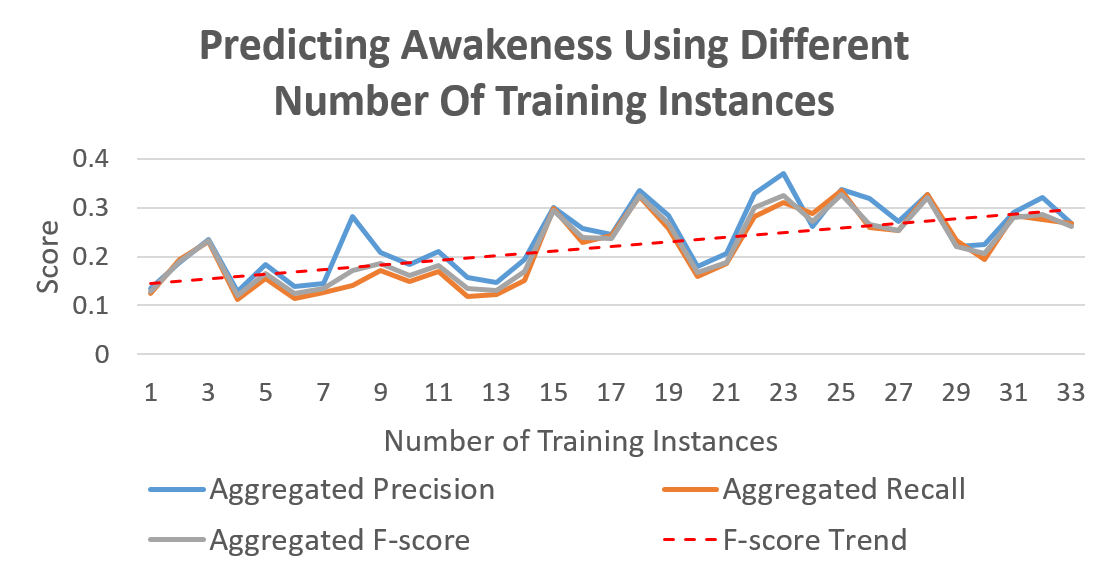
\includegraphics[width=0.5\textwidth]{20180912AwakenessLC2.png}
  \caption{Performance of the per participant trained awakeness classifiers, measured in precision, recall (sensitivity), and F-score. The dotted red line represents the F-score trend.}\label{fig:learningCurveInd}
  %\vspace*{-3mm}
\end{figure}

%\vspace{0.05in}
\noindent\textit{Individual Classifiers for Binary Prediction}\\
The averaged performance of all individually trained random forest classifiers for 'awake' with respect to the training sample size is presented in Figure~\ref{fig:learningCurveInd}. The trend indicates a positive correlation between the number of samples in the training set and the classifiers' F-score performance, with an overall improvement of  114\% (from 0.14 to 0.30) in the F-score between a training set of one sample to one with 33 samples. The trends for
the remaining indicators are 29\% for stress and no overall improvement for focus.%\\[-0.1cm]

%\noindent\textit{}
%When contrasting
%models trained and tested on the 
%biometric data of each user individually, against
%a general model trained and tested with the data of all users. 
%We can conclude
%that for up to 33 training samples analyzed in this study,
%the former has better performance when predicting the
%responses of each user than when training 
%a model with the data of several different users. 
%This is partially due to the 
%variability across users and the subjective nature
%of the responses (e.g.,where slightly awake for one person
%may be not awake for another). 

\begin{figure}
  \centering
      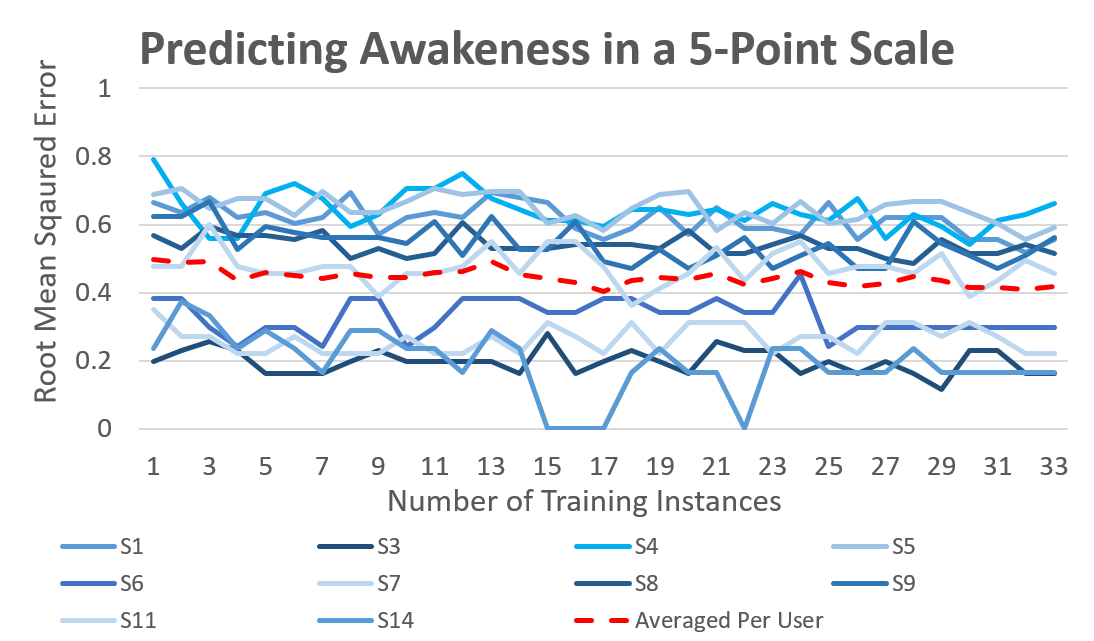
\includegraphics[width=0.5\textwidth]{20180914Awakeness5PointScaleOnly15Lines.png}
  \caption{Performance of the per participant trained classifiers for predicting 5-point awakeness, measured in root mean squared error.}
   \label{fig:learningCurve5}
\end{figure}

\noindent\textit{Predicting Five Classes}\\
In a second step, we analyzed a more fine-grained prediction using the initial 5-point Likert scale responses rather than the binarized ones as output measure. Figure~\ref{fig:learningCurve5} depicts the performance of the individually trained classifiers in terms of the root mean squared error. The root mean squared error represents the distance of the predicted from the actual value, which provides a more nuanced measure of the performance in the fine-grained prediction case. The figure shows a similar trend as for the binarized prediction, in that the root mean square error averaged over all ten participants decreases with more samples (from 0.49 to 0.41 root mean square error) and thus the performance increases. At the same time, the figure also shows that the performance results for the fine-grained prediction, again, vary substantially across participants.

\subsection{Minimum Time Window}\label{secMinimumTW}
In general, the less biometric data is needed to accurately predict a certain outcome measure, the easier and faster the analysis and data collection. To examine the optimal and minimum time window for the prediction of stress, focus, and awakeness, we used 16 different time windows from 10 seconds to 3 hours as depicted in Figure~\ref{timeWindows}. For our analysis, we then trained individual classifiers for each of the 16 time windows, using only features that had a time window smaller or equal to the time window rather than using all combinations of $\{Biometric Measures\} X \{Statistical Metrics\} X \{Time Windows\}$. We again used random forest and a leave-one-out cross validation to train individual classifiers. Since the number of features used for the training changed with each time window, we did not apply our feature selection in this case, but used all features available. Finally, due to the imbalance in the data, we again weighted each participants' classifier performance by the number of instances in the smaller class to calculate the average.

\begin{figure}
  \centering
      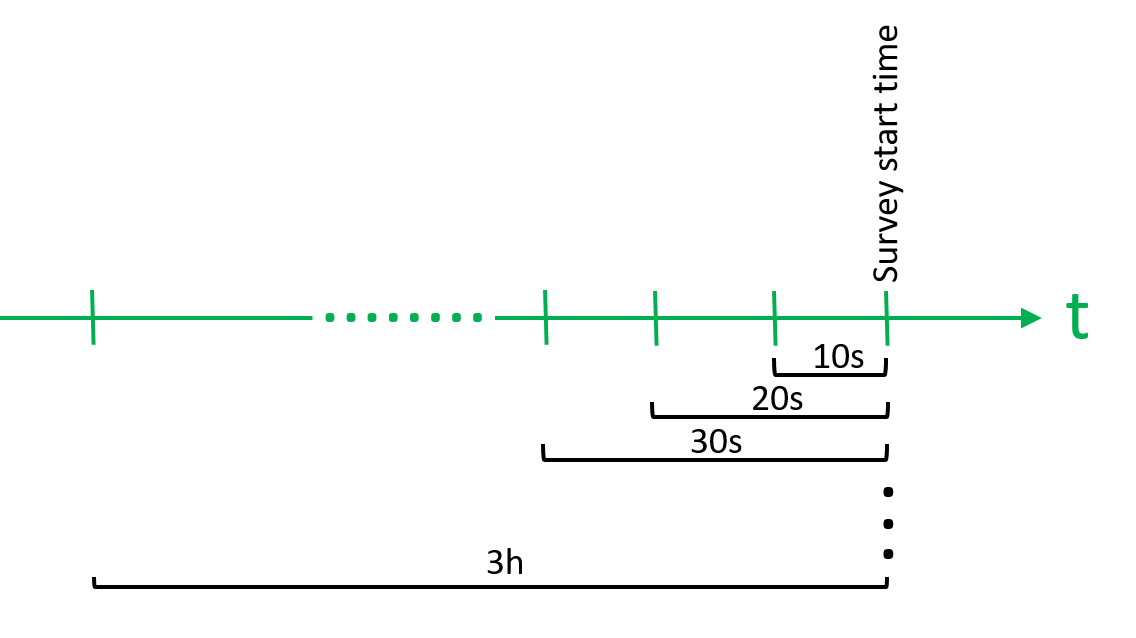
\includegraphics[width=0.4\textwidth]{timeWindows.png}
  \caption{Time windows of biometric data collected prior to each survey response: 10sec, 20sec, 30sec, 45sec, 1min, 2min, 3min, 5min, 7.5min, 10min, 20min, 30min, 45min, 1hour, 2hour, and 3hour.}
   \label{timeWindows}
\end{figure}

Figure~\ref{timeWindowsPandR} shows how the F-score changes for predicting 
`awake' over the 16 different time windows. The figure shows an increasing 
trend in the F-score, i.e. the higher the number of included time windows, 
the higher the F-score. However, there is one exception, the time window of 
1200 seconds that achieves a performance close to the one for the time 
window 10,800 seconds (3 hours), at which point all features are included. 
Overall, our results thus show that while using all time windows up to 3 
hours performs best, and outperforms the feature set that is solely based on 
a 10 second time window by 28\% (from 0.18 to 0.24), the performance for a 
time window of 1200 seconds is a good trade-off for selecting a shorter time 
window while maintaining high performance.

\begin{figure}
  \centering
      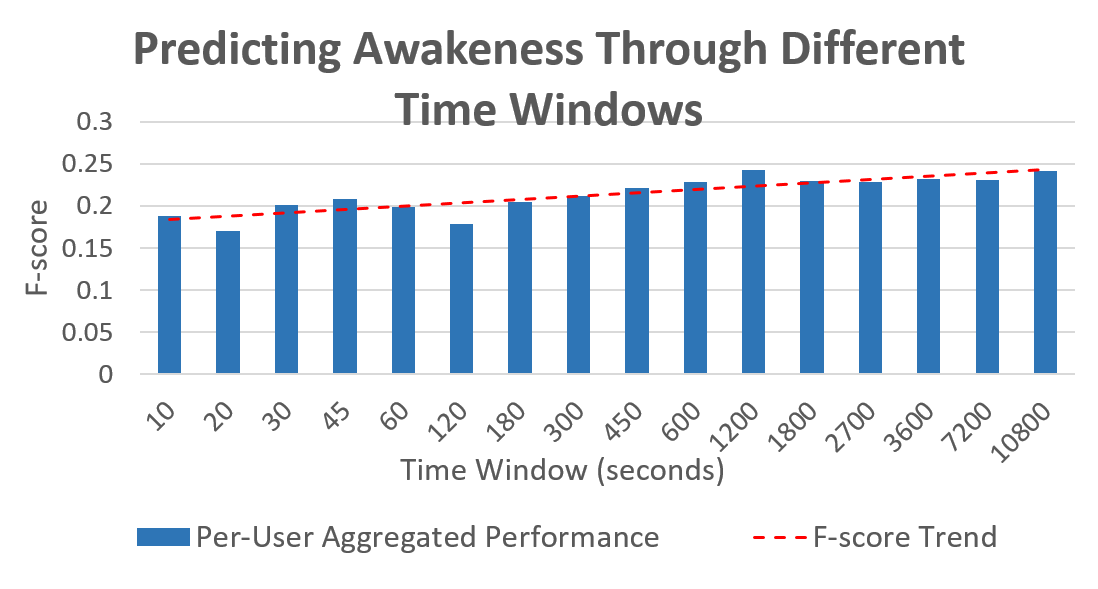
\includegraphics[width=0.5\textwidth]{20180912AwakenessTWBars.png}
  \caption{Performance (F-score) of individual classifiers trained on the different time windows to predict `awake'.}
  \label{timeWindowsPandR}
 % \vspace*{-3mm}
\end{figure}

%We also compared the performance of a model created per user against
%a model created across users.
%To calculate the performance of the model created per user,
%for each user we create a model using the features 
%related to each time window for the selected user only, 
%while in the model created with data across users,
%we trained the model with the data related to each
%particular time window of all users.
%our results show that the personalized model created
%for each user outperforms in every case
%the model created the with data across all users.

%This study
%shows that in general larger time windows predict stress,
%focus, and awakeness more precisely than 
%shorter time windows. We can also notice
%a very gentle upwards trend
%with a inflexion points at 45 seconds and 180.
%There is a peak of performance in 45 seconds, 
%time window that could be used if time is a scarce resource.
%The performance stabilizes around 180 time window
%which indicates that collecting data for a longer time
%period will not increase significantly the performance of the approach.
%The difference in performance between the 
%lowest performing and the highest performing time window is 
%less than a 10\% improvement. 


\subsection{Computer Interaction Data} \label{secCI}
Given our focus on knowledge workers (i.e., workers who generally spend a lot of time interacting with information on their computer at work), we also analyzed the use of computer interaction features to predict focus, awakeness and stress. To collect computer interaction data, we used an open source computer interaction monitor (reference omitted for double-blind.)
%the open source PersonalAnalytics project\footnote{https://github.com/sealuzh/PersonalAnalytics}  \cite{meyer18} 
to track participant's mouse and keyboard activity, as well as details about their active window. The specifics of the features tracked are listed in Table \ref{tracker}. The tracker was installed on the computers of 10 of the 14 participants, with participants S6, S10, S12, and S13 opting out of this part of the study due to privacy concerns.  Therefore, we limited this analysis to the 10 participants for whom we could calculate all features. 

\begin{table}
\begin{center}
\small\addtolength{\tabcolsep}{-1pt}
\begin{tabular}{l l}
\hline

Feature collected by tool & Description \\ 
\hline
Total keystrokes per min& Sum of all types of keystrokes \\ 
Normal keystrokes per min&F[h] Not backspace and navigation \\ 
Backspace keystrokes per min& Backspace keystrokes \\ 
Navigation keystrokes per min& Arrow key keystrokes \\ 
Total clicks per min& Sum of all click types \\ 
Other clicks per min& Not right and left clicks \\ 
Left clicks per min& Left clicks \\ 
Right clicks per min& Right clicks \\ 
Scrolled distance per min& Scrolled distance in pixels \\ 
Moved distance per min& Mouse movements in pixels \\ 
Activity switches per min& Browser window title changes \\ 
Category switches per min& Activity performed category \\ 
\hline
\end{tabular}
\caption{Features collected per user by the computer interaction tracker}%~\cite{meyer18}}
\label{tracker}
\end{center}
%\vspace*{-1mm}
\end{table}

For calculating computer interaction features, we again used the aforementioned 16 time windows and scaled the computer interaction values if the time windows did not align. For our comparative analysis of the different sensing techniques---biometrics vs computer interaction---we then created two new feature sets for each participant in addition to the biometric one: one with only computer interaction features, and one with computer interaction features plus biometric features. 

Table~\ref{ciPerformance} lists the results of our analysis. The results show that in all cases, the computer interaction based model was able to improve upon the biometric model in terms of precision and recall.
%MS is removing the accuracy results because it is not what we care about and it is just making the results harder to understand
%, but not in accuracy. 
Further, we found that the combined model was the most effective model in terms of precision and recall for predicting stress and awakeness overall, but performed slightly worse than the model using only computer interaction features for focus. 
%Since we consider precision and recall for predicting the class of higher interest, i.e. stressed, not focused, not awake, to be the most important statistics when interpreting our results, we compared the models against each other by averaging these two statistics.


\begin{table}
\begin{center}
%\small\addtolength{\tabcolsep}{-1pt}
\begin{tabular}{llllll}
\hline
Model/Feature Set & Precision & Recall & F-Score \\ %& Accuracy\\
\hline
\textbf{Awakeness}\\
\hspace{3mm}Biometrics only  & 0.269 & 0.314 & 0.289 \\ %& 0.808\\
\hspace{3mm}C.I. only  & 0.425 & 0.362 & 0.391 \\ % & 0.758\\
\hspace{3mm}Biometrics + C.I. & 0.390 & 0.404 & 0.400 \\ % & 0.791 \\
\hline
\textbf{Stress}\\
\hspace{3mm}Biometrics only  & 0.270 &	0.260 & 0.265 \\ % & 0.775\\
\hspace{3mm}C.I. only & 0.290 & 0.272 & 0.281 \\ % & 0.698 \\
\hspace{3mm}Biometrics + C.I. & 0.317 & 0.286 & 0.301 \\ % & 0.712\\
\hline
\textbf{Focus}\\
\hspace{3mm}Biometrics only & 0.251 & 0.256 & 0.253 \\ % & 0.716\\
\hspace{3mm}C.I. only & 0.332 & 0.342 & 0.337 \\ % & 0.742\\
\hspace{3mm}Biometrics + C.I. & 0.340 & 0.316 & 0.328 \\ % & 0.745\\
\hline
\end{tabular}
\caption{Comparison of the performance of predicting stress, focus and awakeness using the 3 different feature sets for the 10 participants. The performance is calculated as the average of the performance of the individual classifiers. Computer Interactions is abbreviated as C.I. here for readability. Precision and recall refer to the prediction of the more important classes, i.e. `stressed', `not awake', `not focused'.}
\label{ciPerformance}
\end{center}
%\vspace*{-1mm}
\end{table}

As with the biometric models, the individual performance of both the computer interaction only models and the combined models varied quite a bit between participants. Using stress as an example again, in the computer interaction models 5 of the 10 participants saw improvements compared to the baseline, with a maximum improvement of 128\% in precision, and 78\% in recall. In the combined model for stress, 5 of the 10 participants saw improvements compared to the baseline, with a maximum improvement of 117\% in precision and 95\% in recall. Neither model was capable of correctly predicting any instances of 'stressed' for participant S7.

Since the number of features changes  depending on which feature set is used, we adjusted the feature selection parameter for each of the computer interaction and combined computer interaction/biometric models. The values reported in this section were achieved using the optimal feature selection parameters we found, which are shown in Table \ref{ciFeatureSelection}.

\begin{table}
\begin{center}
\begin{tabular}{lc}
\hline
Model/Feature Set & Number of Features Selected\\
\hline
\textbf{Stress}\\
\hspace{3mm}C.I. & 400\\
\hspace{3mm}Biometrics + C.I. & 800\\
\hline
\textbf{Focus}\\
\hspace{3mm}C.I. & 20\\
\hspace{3mm}Biometrics + C.I. & 300\\
\hline
\textbf{Awakeness}\\
\hspace{3mm}C.I. & All\\
\hspace{3mm}Biometrics + C.I. & 50\\
\hline
\end{tabular}
\caption{The optimal number of features we found to select for each of the model/feature set combinations. Computer interactions is abbreviated as C.I.}
\label{ciFeatureSelection}
\end{center}
\vspace*{-4mm}
\end{table}



%\section{Analysis and Results}

%% To evaluate the efficacy of continuously predicting a knowledge worker's stress, focus, and awakeness in the workplace, we trained and tested machine learning classifiers using a leave-one-out cross validation. For prediction, we used the features extracted from the collected data as the input data, and binarized the participants' self-reported responses on stress, focus, and awakeness into two classes each (e.g., 'stressed' and 'not stressed') to use as output measures.

\section{Observed Trends Over Time in Stress and Awakeness Levels}
\label{stressTrends}

To gain insights into how knowledge workers experience stress and awakeness over an
extended period of work, we examined the end of day survey responses
collected from each participant to see if any identifiable trends
emerged. As we noted in the last section, we did not ask
participants about focus in the end of  day surveys as focus is an 
aspect relevant at a particular moment in time rather than an aspect
for an extended period of work. We used data from 13 of the 14 participants - we excluded one participant
from this analysis as they experienced atypical stress
levels in the latter half of the study due to factors outside of our
control.

\subsection{Stress Levels}
Overall, we identified three prominent characteristics in the stress levels.
%\rev{We describe characteristics noted in the reporting of the knowledge workers about the stress they experienced over the duration of the study.}

\begin{figure}[h!]
  \centering
      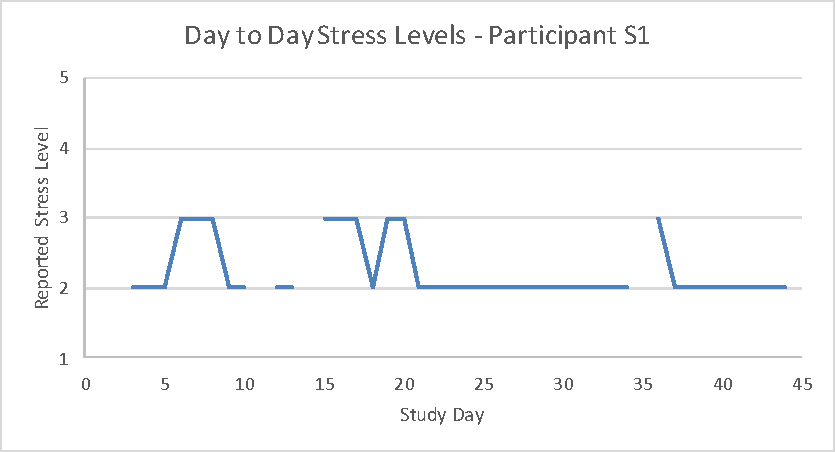
\includegraphics[width=0.7\textwidth]{s1_stress.pdf}
      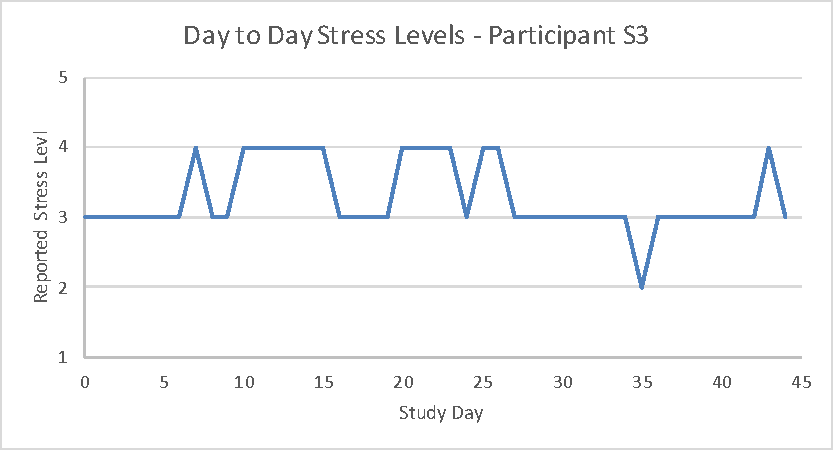
\includegraphics[width=0.7\textwidth]{s3_stress.pdf}
  \caption{The day-to-day stress levels reported by two participants (S1 and S3) are shown. The y-axis represents values on the 5-point Likert scale we asked participants to respond with ranging from 1/Not at all stressed to 5/Extremely stressed. The x-axis represents the day of the study on which the value was recorded (from 0-45). Some gaps are present in the chart for S1 as they did not report their stress level on those days.}
   \vspace*{-2mm}
   \label{fig:dailyStress}
\end{figure}


\subsubsection{Baseline Stress Levels}
%\noindent\textit{\textbf{Baseline Stress Levels.}}
Common amongst all participants was a trend to select one stress rating
far more frequently than any other. We will refer to this value as the
participant's baseline stress level. All but one participant reported
their perceived stress level for the day as their baseline stress
level more than 50\% of the time. In total, the baseline values made
up 65\% of the reported values collected from
participants. Interestingly, while participants sometimes saw periods
of sustained increases in stress, lasting as many as 6 consecutive
workdays in the most extreme case, participants would always return to
their baseline stress level at some point.


The baseline stress level varied significantly between participants. \rev{Seven}
participants (54\%) reported feeling average stress levels most frequently
(rating 3 on our scale), while \rev{five} (38\%) reported feeling little stress
(rating 2) and \rev{one} (8\%) reported feeling no stress at all (rating 1). Figure \ref{fig:dailyStress} illustrates these points using  data from two participants, showing the tendency to report and return to baseline stress levels, as well
as a distinct difference in baseline stress level (rating 2 for S1 vs rating 3 for S3). Gaps in the chart for S1 represent days for which the participant did not report their stress level.


\subsubsection{Stressful Days Tend to Cluster}
Accounting for the variance between participants perceived stress
baselines, we consider a stressful day to be one that represents a
deviation of \rev{one} or more stress levels above the participant's
baseline. Of the 93 stressful days we observed in total, we found that
39 (41\%) of these days occurred in groupings of two or more
consecutive stressful workdays. The most common size of these groups
was two workdays, while the largest group we observed was six
workdays.  The day after a stressful day is much more likely to be a
stressful day as compared to any other day with a 0.55 average increase
over baseline, compared to 0.02 average increase over baseline.

\subsubsection{Extreme Changes in Stress Levels are Rare}
After accounting for each participant's perceived stress baseline, we
examined the frequency of deviations from the baseline. We found that
participants were far more likely to report a stress level that was
within \rev{one} point of their baseline, than to report a stress level 2 or
more points away. These extreme deviations represented only 15\% of
all reported values, which differed from the \rev{participant's} baseline. As
well, the majority (78\%) of these deviations came from just two
participants. This suggests that some people may be less resilient to
the stress of the workplace than others. For most participants,
extremely stressful days were few and far between.

\subsection{Awakeness}
We applied the same analyses described above to the \rev{self-reported} awakeness levels of our participants. Compared with the reported stress levels, we observed the same trend of participants reporting one baseline far more commonly than any other. We did not find there to be a significant correlation between reported stress and awakeness levels. Overall, \rev{participant's} awakeness levels fluctuated significantly less than their stress levels (73.1\% of reports were at the baseline level, compared to 65.1\% for stress, p < 0.05). Participants were unlikely to experience days with heightened (above baseline) awakeness. Such days made up only 6.0\% of the total observed \rev{workdays} across all participant. Most of these days came from one participant, S2, who reported 15 heightened awakeness days compared to the next highest, S13 with four. Large deviations (>1 point deviation) from each participants baseline awakeness levels were extremely uncommon, accounting for only \rev{nine} (2.1\%) of our total observations. Similarly to what we observed with high stress days, low awakeness days frequently came in clusters of two or three days in a row. Given that the immediately preceding day was a low awakeness day\rev{;} a given day was 228.2\% more likely to be a low awakeness day than when considering any day at random (p < 0.0001).


\begin{table}[]
    \centering
\rev{\begin{tabularx}{\textwidth}{|c|c c c|c c c|}
    \hline
        &
        \multicolumn{3}{c|}{Stress} & 
        \multicolumn{3}{c|}{Awakeness} \\
        \hline
        \textbf{Variable} & \centering
        \textbf{\rev{F.E.E.}}& \textbf{p-value} & \textbf{\rev{C.I. (95\%)}} & \centering \textbf{\rev{F.E.E.}}  & \textbf{p-value} & \textbf{\rev{C.I. (95\%)}}\\
        \hline
        Monday & \centering -0.033 & 0.745 & \rev{$(-0.234, 0.167)$} & \centering -0.058 & 0.497 & \rev{$(-0.227, 0.110)$}\\
        Tuesday & \centering 0.028 & 0.773 & \rev{$(-0.164, 0.221)$} & \centering 0.036 & 0.662 & \rev{$(-0.126, 0.198)$}\\
        Wednesday & \centering 0.163 & 0.100 & \rev{$(-0.031, 0.357)$} & \centering -0.018 & 0.830 & \rev{$(-0.181, 0.145)$}\\
        Thursday & \centering 0.022 & 0.821 & \rev{$(-0.169, 0.213)$} & \centering 0.076 & 0.927 & \rev{$(-0.085, 0.238)$}\\
        Friday & \centering 0.082 & 0.473 & \rev{$(-0.142, 0.306)$} & \centering -0.178 & 0.025 & \rev{$(-0.334, -0.022)$}\\
        Month End & \centering 0.044 & 0.687 & \rev{$(-0.171, 0.259)$} & \centering -0.082 & 0.374 & \rev{$(-0.263, 0.099)$}\\
        \hline
    \end{tabularx}
    \caption{\rev{Fixed effects estimates (F.E.E.), 95\% confidence intervals and associated p-values for the explanatory variables (day of week and proximity to month end) that we examined in our linear mixed model analysis.}}    \label{tab:mixedModel}}
\end{table}





\subsection{Explaining Fluctuations}
In an attempt to explain some of the fluctuations in stress and awakeness that our participants were experiencing, we created a linear mixed model with the self-reported daily stress and awakeness levels as dependent variables and the participants as random effects. We experimented with day of the week and proximity to beginning or end of month as possible explanatory variables. Ultimately, the analysis showed that none of the variables that we examined had a significant explanatory power with respect to our participants perceived stress levels.
For awakeness, we found  that there was a small (\rev{fixed effects estimate}: -0.178) yet significant decrease in awakeness levels on Fridays in particular. Table \ref{tab:mixedModel} shows some of the detailed results of these analyses. These results show the difficulty of explaining a person's stress and awakeness via simple measures, and point to the need for additional instrumentation and data collection if we are to successfully understand and make predictions about these human aspects in the workplace.




\section{Predicting Stress, Focus and Awakeness in the Moment}
% random forest best
\label{secOverallAccuracy}

To investigate whether stress, focus and awakeness can be predicted in
the moment based on biometric measures,
we investigated classifiers trained
for each individual and across all participants. We report on the effectiveness of
these classifiers and the features that are important in predicting stress, focus
and awakeness.

\subsection{Data Preparation}

\rev{In a machine learning context, data preparation and utilization is an essential part of the proposed solution. To prepare} the collected data for use in training and testing \rev{our proposed} machine learning models, we performed \rev{the following} steps.


\subsubsection{Data Cleaning}
All data recorded by the Everion is associated with a quality score ranging from 0-1 that is calculated using proprietary methods. In accordance with the recommendations of Biovotion,
to prevent our results from being effected by erroneous data we set a quality threshold of 0.5 and discarded any data gathered which had a quality rating below this threshold. 

\subsubsection{Data Linking}

We linked the collected biometric data and survey responses for each participant. Linking the data is necessary to construct training and test datasets for use in creating and evaluating machine learning models.

To link the data, we look back one hour from the start time of each survey response for
available biometric data.  For example, if a participant started a survey response at 11:05am, we look for biometric data from between 10:05am to 11:05am. If no biometric data was recorded in the hour time window, we exclude the survey response from the dataset. Otherwise, we consider the survey response to have associated biometric data.

There are several reasons for a survey response to lack associated biometric data:
\begin{itemize}
\item The participant was not wearing the Everion in the hour before beginning the survey.
\item The Everion was not recording data in the hour before the participant began the survey (e.g., due to low battery).
\item Biometric data was not being uploaded successfully to the server.
%\item Compatibility issues between the sensor and the OS tracking the participant's data
%\item Issues accessing the data uploaded by the participants
\end{itemize}

Figure~\ref{surveyBio} illustrates the number of survey responses with associated biometric data for each study participant. 
%This was added to address REviewer 2's concern: Is it correct that the maximum number of responses should have been 112 on the surveys?
The total number of responses per participant is affected by their response rate and by the number days out-of-office (e.g., vacations, holidays, etc.). 
Participant S2 and S12 have particularly low numbers of usable survey responses. In each of these cases, the issue related to biometric data not being uploaded successfully to the server.

\begin{figure}
  \centering
      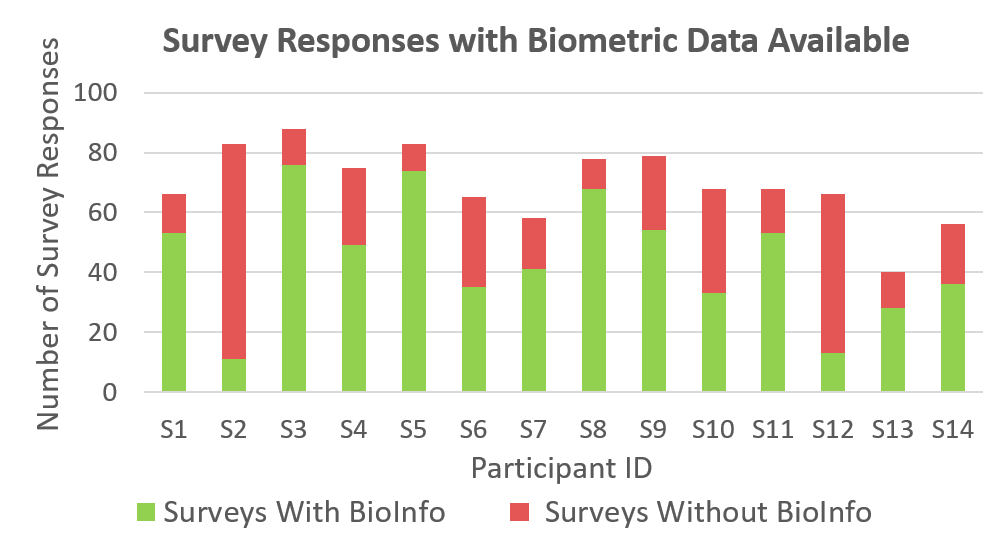
\includegraphics[width=0.8\textwidth]{DuringTheDay.png}
  \caption{The figure shows the biometric data available per each participant. Green sections represent survey responses with biometric
  data available, red sections responses with no biometric data available}
   \label{surveyBio}
   \vspace*{-4mm}
\end{figure}


\subsubsection{Feature Extraction}
We extracted features from the biometric data to provide as input to machine 
learning models. Previous 
studies~ \cite{vorburger05,zuger2015interruptibility} identify time windows as an 
important factor that impacts the prediction accuracy of a classifier. We 
considered many time windows from the literature on biometric 
analysis~\cite{zuger18}, ranging from 10 seconds to 3 hours. Specifically, we 
considered the following time windows: \textit{10sec, 20sec, 30sec, 45sec, 
1min, 2min, 3min, 5min, 7.5min, 10min, 20min, 30min, 45min, 1hour, 2hour, 
3hour}.

From the start time of each survey response, we look back the amount of time 
that corresponds to each time window and we create features for all of the 
biometric data available in that time window. For example, if a participant 
started a survey response at 11:05am, for the 30min time window, we create 
features using all of the available biometric data from 10:35am to 11:05am. 
If there is a large portion ($\geq$50\%) of data missing (either because of a recording issue or because of low quality data) from the time window considered, then the time window is marked as missing. In this case, features are imputed based on the mean of other samples of the same feature for that participant. This is an effective and commonly used technique, which is preferable to the alternative of deletion as it preserves our already small sample size~\cite{hawthorne2005imputing}.
For each time window, we calculate 10 statistical measurements from the 
biometric data to create 10 distinct features. Specifically, the 10 
statistical measurements are: mean, standard deviation, variance, median, 
25\textsuperscript{th} percentile, 75\textsuperscript{th} percentile, interquartile range, maximum, minimum, and 
range. Thus, for each survey response, we generate a large number of 
corresponding features based on three factors: biometric measurement, time 
window, and statistical measurement. In addition to these biometric 
features, we also considered the time of day in which the questions were 
asked. These features are created to predict the responses described by the 
ground truth. To attempt to account for inter-participant differences, we normalized all features on a per-participant basis.

\begin{table}
  \centering
      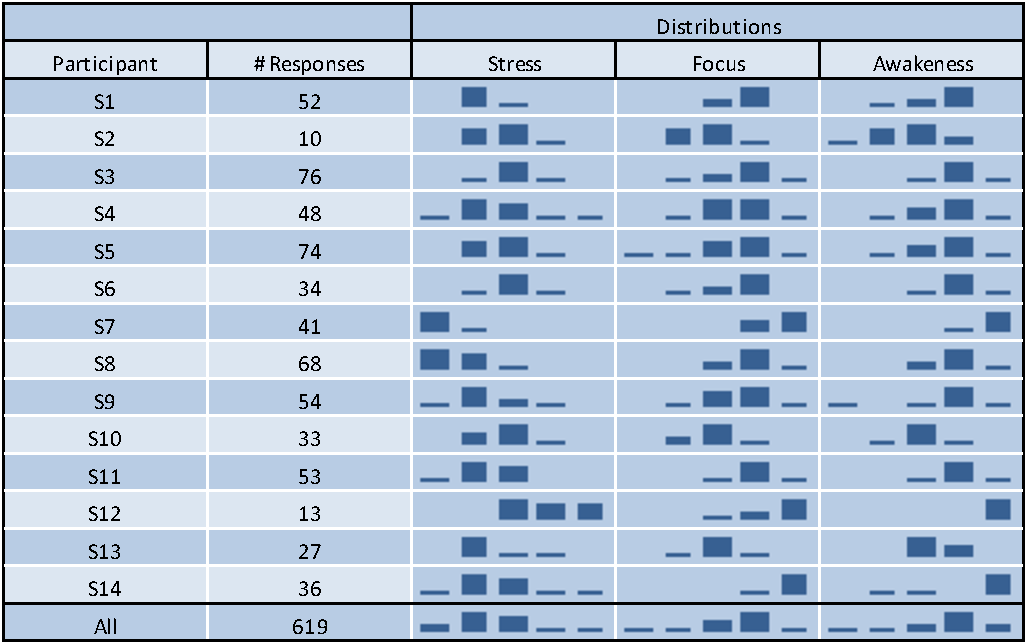
\includegraphics[width=0.8\textwidth]{distributiontable.pdf}
  \caption{The distribution of the responses of each participant to the three questions asked during the day are shown. Each bar in the histograms represent one of the \ref{five} values on the 5-point Likert scale we asked participants to respond with, where the far left side of the histograms are 1/Not at all, and the far right sides are 5/Extremely}
   \label{responseDistribution}
   %\vspace*{-2mm}
\end{table}

\subsubsection{Response Transformations}
Table~\ref{responseDistribution} illustrates the distribution of responses from each participant for each of the three survey questions (listed in Section~\ref{sec:Surveys}). The figure shows that there is a notable imbalance in the distribution of the self-reported responses provided by the participants. Most participants did not use all five points of the five-point Likert scale in their responses, and the distributions tend to skew toward one side or the other, depending on the question. Given 
this distribution and based on our earlier observation that the participants tended to adhere to a baseline reporting level for stress and awakeness, we elected to simplify the problem from \rev{five} classes to \rev{two}. This transformation enables us to more easily represent patterns in the data, such as when a participant fluctuates from a normal to high stress level. To perform this transformation, \rev{we began by calculating the median response value for each participant and each question}. We classified each response below the median as 0 (`negative') and each response above the median as 1 (`positive'). The distribution for the stress question skewed left, so we included the median values in the `positive' class (i.e. `stressed'), while the distributions for focus and awakeness skewed right, so we included those median values in the `negative' class (i.e. `not focused', `not awake').

With this method, we transformed the survey data into a two-point scale, representing  negative or positive responses for each of the three human aspects of interests (e.g., not stressed or stressed). 

\subsubsection{Oversampling}
Even after binarizing the responses as described in the previous section, we found the distribution of responses was still quite imbalanced for many of our participants. This can be seen in the distribution columns in Table \ref{tab:accuracy}. To mitigate this effect, we applied random oversampling to our training sets, which artificially rebalances the dataset by creating randomly replicated data in the minority class. This technique has commonly been used  in previous studies on unbalanced datasets \cite{chawla2004,yap2014}.

\begin{comment}
\begin{table}[h]
	\begin{centering}
	\small\addtolength{\tabcolsep}{-1pt}
    \begin{tabular}{llll}
      \hline
      Variable & K & \# Estimators & Minimum Samples Split \\
      \hline
      Stress & 300 & 100 & 4\\
      Focus & 200 & 50 & 4\\
      Awakeness & 800 & 100 & 4\\
      \hline
    \end{tabular}
    \caption{The hyperparameters selected by grid search analysis to tune our random forest models. K refers to the number of features selected.}    \label{tab:hyperparams}
    \end{centering}
\end{table}
\end{comment}


\subsection{Selecting a Classifier Algorithm}

\rev{Many different algorithms can be used to build a classifier.} To select an
algorithm, we compared multiple classifiers using the popular machine learning library scikit-learn~\cite{pedregosa11},  evaluating each one by using leave-one-out cross validation. Our analysis showed that random forest outperforms all other classifiers, including Na\"ive Bayes, decision trees, support vector machine, and a multilayer perceptron neural network. For the remainder of this paper, we refer to a random forest classifier.%\\[-0.1cm]
% for stress they were (minimum samples for split = 4, # of estimators = 100, max features = 0.5, k=300), for focus they were (minimum samples for split = 4, # of estimators = 50, max features = 0.5, k=200), and for awakeness they were (minimum samples for split = 4, # of estimators = 100, max features = 0.25, k=800)



\begin{table*}[h]
  \centering
  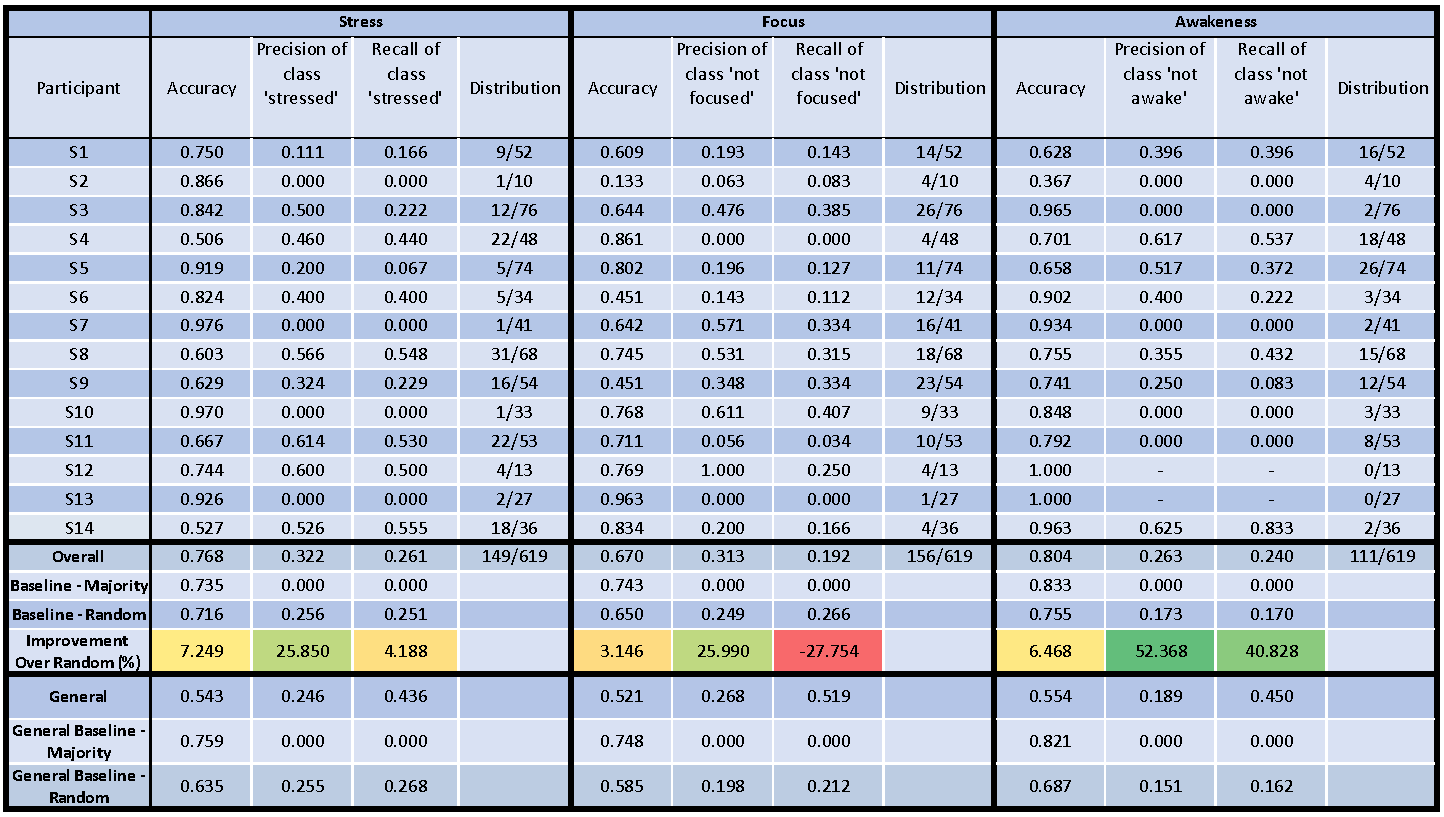
\includegraphics[width=1.0\textwidth]{rq1performance_v2.pdf}
  \caption{Results of predictions using the individual models. The distribution columns show the proportion of the minority class out of the total number of responses for each of the three variables. The baseline rows represents the averaged results of our baseline classifiers. The general row shows the averaged results of our models trained on all participants.}\label{tab:accuracy}%\todo{revise caption}}
  \vspace*{-4mm}
\end{table*}

\subsection{Individual Classifiers}
%\noindent\textit{Results of Individual Classifiers}\\
Since peoples' experience of stress, focus, and awakeness (as well as
their physiological manifestations) can vary substantially
(e.g.,~\cite{Hernandez11}), we first trained and evaluated individual classifiers
for each participant (as opposed to a general one for all
participants) using leave-one-out cross validation. The results of our analysis are reported in
Table~\ref{tab:accuracy}. For our analysis, we report values of
accuracy, one of the most commonly used metric to compare performance,
as well as precision and recall of the classes of interest:
`stressed', `not focused', and `not awake'. Since the imbalance in the
data can lead to high accuracy values if a classifier always just
predicts the most likely/frequent class while ignoring the class of
higher importance and interest, precision and recall of the class of
interest are also important to
consider~\cite{yap2014,bhattacharyya_data_2011,Hernandez11}.

\rev{Besides} our results, for the purposes of comparison\rev{,} we also present two commonly used baselines in this table - a majority classifier, which always predicts the larger of the two classes considered, and a stratified random classifier which randomly chooses between the two classes, but with a proportional bias towards the larger class.

For some users (i.e., S1. as seen in Table \ref{responseDistribution}), the imbalance in their data was so extreme that even after adjusting by oversampling\rev{, we were not able} to create a reasonable classifier. These scenarios are difficult to predict\rev{,} as any classifier will not have enough variance in its training data for the 'stressed' situation to adequately distinguish it from the non-stressed case.


% However, the imbalance in the data can lead to a classifier with high accuracy if it always just predicts the more likely class while ignoring the class of higher importance and interest in our case (i.e. stressed, not focused, not awake). Therefore, we further report the precision and recall for the three classes 'stressed', 'not focused' and 'not awake'. 


Overall, we were able to use extracted physiological features to
predict all three aspects with reasonable accuracy, precision, and
recall. We present a comparison between the averaged results of our individual classifiers and those of the baseline stratified random \rev{classifier} in the ``Improvement Over Random'' row of Table \ref{tab:accuracy}. This is calculated as the difference between the overall average and the baseline results, divided by the baseline results (for example, $\frac{Acc_{Overall} - Acc_{Random}}{Acc_{Random}}$). We do not compare our results with the majority classifier directly as this classifier achieved precision and recall scores of zero when predicting stress, lack of focus, and lack of awakeness, making a meaningful comparison \rev{unfeasible}. The improvement percentages demonstrate that the predictions made by our classifiers are much better than random after correcting for the imbalance in our dataset.

While the individually trained classifiers
improved on average across all participants upon the baseline in all
cases except in recall of `not focused', the improvement was
substantially higher for awakeness (52.4\% improvement in precision,
40.8\% in recall, and 6.5\% in accuracy) than for stress or focus. In addition,
the performance of the individually trained classifiers varied greatly
across participants. While some participants showed a large
improvement, for others the baseline performed much better than the
individually trained classifier. For instance, for predicting
`stressed', the individual classifiers improved upon the baseline for
S4, S6, S8, S11, S12, and S14 with a maximum improvement of 152.0\% in
precision and 111.1\% in recall for S12, while they did worse for S1,
S3, S5, S7, S9, S10, and S13, and in the worst cases did not correctly
predict a single instance of `stressed'. Typically, users that have the
lowest precision and recall values are those where the data is the
most imbalanced.\\[-0.1cm]
% We attribute these discrepancies to the large differences in response distributions between participants, as well as to the subjectivity of self-reporting.
%
%(improvement: 8\% precision, 1\% recall, 8\% accuracy), the individual performance varied greatly among participants. Some participants showed negligible difference in comparison to the baseline classifier, e.g. subject ..., while others showed a large improvement, e.g. subject ...
%\begin{table}[h!]
%\begin{centering}
%\begin{tabular}{lll}
%\hline
%Participant & Recall Improvement (\%) & Precision Improvement (\%)\\
%\hline
%S12 & 184.6 & 88.4 \\
%S6 & 66.7 & 85.8 \\
%S11 & 50.0 & 44.4 \\
%S8 & 32.4 & 26.7 \\
%S14 & 14.7 & 9.8 \\
%S4 & 5.6 & 5.5 \\
%S9 & -55.4 & -46.8 \\
%S3 & -90.0 & -82.1 \\
%S1 & -100.0 & -100.0 \\
%S5 & -100.0 & -100.0 \\
%S7 & -100.0 & -100.0 \\
%S10 & -100.0 & -100.0 \\
%S13 & -100.0 & -100.0\\
%S2 & - & -\\
%\hline
%\end{tabular}
%\caption{Percentage improvement in recall and precision for stress, using our approach compared to the baseline, on an individual level. For participant 2, the baseline achieved a precision and recall of 0, thus the improvement is undefined}
%\end{centering}
%\label{tab:indImprovement}
%\end{table}


\subsection{Feature Selection and Importance}
%\noindent\textit{Feature Selection and Importance}\\
There are a large variety of features that can be (and have been) calculated in previous research for each of the basic measurements listed in Table~\ref{signals}, such as the mean, standard deviation, maximum, and interquartile range. In addition, each of these metrics can be combined with the various time windows captured of a basic measurement, resulting in a large feature space. To reduce the feature space, we experimented with multiple feature selection methods, including selecting the top k highest correlated features by various metrics such as mutual information, Pearson's correlation coefficient, ANOVA's F-value, as well as wrapper methods such as recursive feature elimination, optimizing mean decrease accuracy by iteratively permuting features, and only selecting features that exceed a certain Gini importance threshold. We found that all methods produced similar results with respect to accuracy, precision, and recall for the individual models. Ultimately, we elected not to utilize any feature selection in order to simplify our approach, as we found there to be minimal differences in performance between the techniques, and the random forest algorithm is capable of (and robust for) handling datasets with many features.

%Respiration rate is also highly important for stress (#3 , 14.4%) but I'm not sure what previous works say about correlation with stress
Overall, the features that were selected as the important ones for the individual models based on the random forest algorithm varied greatly across participants. Yet, some feature categories were considered to be important more frequently than others. Table~\ref{tab:featureImportance} shows the averaged Gini importance for the feature categories used for predicting stress. Heart rate variability proved to be an important measure for all of the aspects of interest, ranking as the most important feature category for both stress and awakeness, and the second most important one for focus. This is not surprising, as heart rate variability and skin temperature have been shown in several previous studies to be possible indicators for stress levels~\cite{dishman2000stress,mcduff16,kataoka00}. We also found blood pulse wave to be an important indicator for both focus and awakeness, but less important for stress, while respiration rate was important in stress and focus but not awakeness. Besides these mentioned feature categories, there was great variation in which measures were important to which of the three aspects. This shows that there is a clear benefit to having multiple biometric streams available for predicting stress, focus and awakeness.\\[-0.1cm]


\begin{table}[h!]
  \begin{centering}
  \begin{tabular}{llll}
    \hline
    Feature Category & Stress & Focus & Awakeness\\
    \hline
    Heart Rate Variability & 18.3\% & 13\% & 13.6\%\\
    Blood Pulse Wave & 10\% & 14.2\% & 13.1\%\\
    Heart Rate & 8.7\% & 12.6\% & 10.3\%\\
    Skin Temperature & 15.7\% & 9.8\% & 10\%\\
    Galvanic Skin Response & 6.6\% & 8.2\% & 5.1\%\\
    Respiration Rate & 14.8\% & 12.7\% & 10\%\\
    Oxygen Saturation & 5.6\% & 4.3\% & 2\%\\ 
    Energy Expenditure & 6\% & 7.7\% & 4.8\%\\
    Activity & 4.6\% & 7.8\% & 7.6\%\\
    Steps & 1.7\% & 0.8\% & 0.9\%\\
    Time of Day & 0\% & 0.1\% & 0.5\%\\
    \hline
  \end{tabular}
  \caption{The averaged Gini importance of each feature category, per response variable.}
  \label{tab:featureImportance}
  \end{centering}
  \vspace*{-2mm}
\end{table}

\subsection{Individual vs.\ General Model}
%\noindent\textit{Individual vs.\ General Model}\\
Individual models are trained specifically for each individual and thus require a data collection period before they are capable of making accurate predictions. On the other hand, the idea of general models is to be able to train them on already collected data and then  to be able to apply them even to new and unseen individuals, thus overcoming the cold-start problem. Given the large individual differences in biometrics, training a general model to achieve an adequate accuracy for new individuals is not necessarily possible. 

To examine the performance of a general model for our participants, we trained three general models, one for focus, one for awakeness and one for stress. We roughly followed the same procedure as for the individual models. Due to the larger amount of data available in the general case, we used the more common random undersampling, which randomly selects elements in the majority class to exclude from the dataset, instead of random oversampling to balance the distribution of the dataset. The models were trained on the datasets of 13 of the 14 participants, and then evaluated on the dataset of the last (leave-one-participant-out cross-validation), repeating this process for all 14 participants. 

The bottom \rev{three} rows of Table \ref{tab:accuracy} present the averaged performance results for this approach in terms of accuracy, precision, and recall, as well as the results of baseline stratified random and majority classifiers following the same leave-one-group-out cross-validation procedure. Although the averaged precision and recall are comparable or better than those of the averaged individual results, this was at the cost of a large decrease in overall accuracy.  Upon closer investigation into the performance of the general model when testing on each participant, we found that individually trained models for each participant performed much better than a general model trained over all participants. Using stress as an example, for participant S12, for whom we saw the greatest increase compared to the baseline in individual models, the general model was unable to predict a single instance of `stressed' correctly. This is consistent with our expectations because biometric features are highly specific to individuals.


%\todo{put the content of the following sentence somewhere into the discussion; We attribute these discrepancies to the large differences in response distributions between participants, as well as to the subjectivity of self-reporting.}


%%%!TEX root = bioPrediction_main.tex

\subsection{Minimum Number of Training Samples}\label{secLearningCurve}
Collecting experience samples from users is expensive, since participants 
are being interrupted several times a day and have to answer the survey. 
To minimize the number of samples to be collected from participants, we 
examined how the performance of individual classifiers changes over the 
number of samples used to train the classifier.

Participants in our study had varying levels of responsiveness to the 
experience sampling ranging from 10 to 76 (see Figure~
\ref{responseDistribution}).
%Answering Reviewer 2's concern: Why only 10 participants? What was the rationale for the cut-off selected? 
To answer this research question we analyze the maximum number of responses \textbf{all} analyzed participants have to train the model. Since some participants have a very small number of maximum answers (ten being the lowest) we excluded the four participants with the least number of responses for this analysis.
%To maintain a certain generalizability while 
%also being able to examine a range of sample numbers for training the 
%classifier, we removed the four participants with the least number of 
%samples for this analysis. 
As a result, we obtained a corpus of analysis where all participants have a 
higher number of responses (34 being the lowest), which allows us to examine 
the learning curve of the classifiers for a larger number of training data points. For our 
analysis, we thus performed a leave-one-out cross validation with random 
sample sets of size 1 to 33 and calculated the average through all folds of 
the validation.

For each of the three productivity-related aspects, we are again more 
interested in predicting when a worker is stressed, not awake, or not 
focused, the less common class in all three cases. Since the less common 
class can be very small, we weighted each participants' classifier 
performance by the percentage of the samples in this smaller class.

\begin{figure}
  \centering
          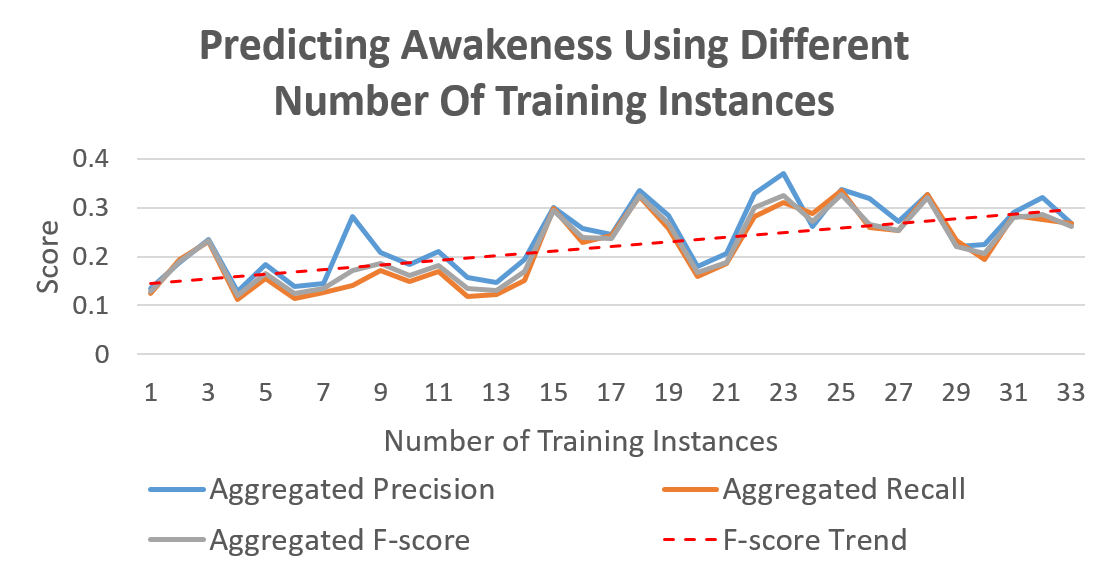
\includegraphics[width=0.5\textwidth]{20180912AwakenessLC2.png}
  \caption{Performance of the per participant trained awakeness classifiers, measured in precision, recall (sensitivity), and F-score. The dotted red line represents the F-score trend.}\label{fig:learningCurveInd}
  %\vspace*{-3mm}
\end{figure}

%\vspace{0.05in}
\noindent\textit{Individual Classifiers for Binary Prediction}\\
The averaged performance of all individually trained random forest classifiers for 'awake' with respect to the training sample size is presented in Figure~\ref{fig:learningCurveInd}. The trend indicates a positive correlation between the number of samples in the training set and the classifiers' F-score performance, with an overall improvement of  114\% (from 0.14 to 0.30) in the F-score between a training set of one sample to one with 33 samples. The trends for
the remaining indicators are 29\% for stress and no overall improvement for focus.%\\[-0.1cm]

%\noindent\textit{}
%When contrasting
%models trained and tested on the 
%biometric data of each user individually, against
%a general model trained and tested with the data of all users. 
%We can conclude
%that for up to 33 training samples analyzed in this study,
%the former has better performance when predicting the
%responses of each user than when training 
%a model with the data of several different users. 
%This is partially due to the 
%variability across users and the subjective nature
%of the responses (e.g.,where slightly awake for one person
%may be not awake for another). 

\begin{figure}
  \centering
      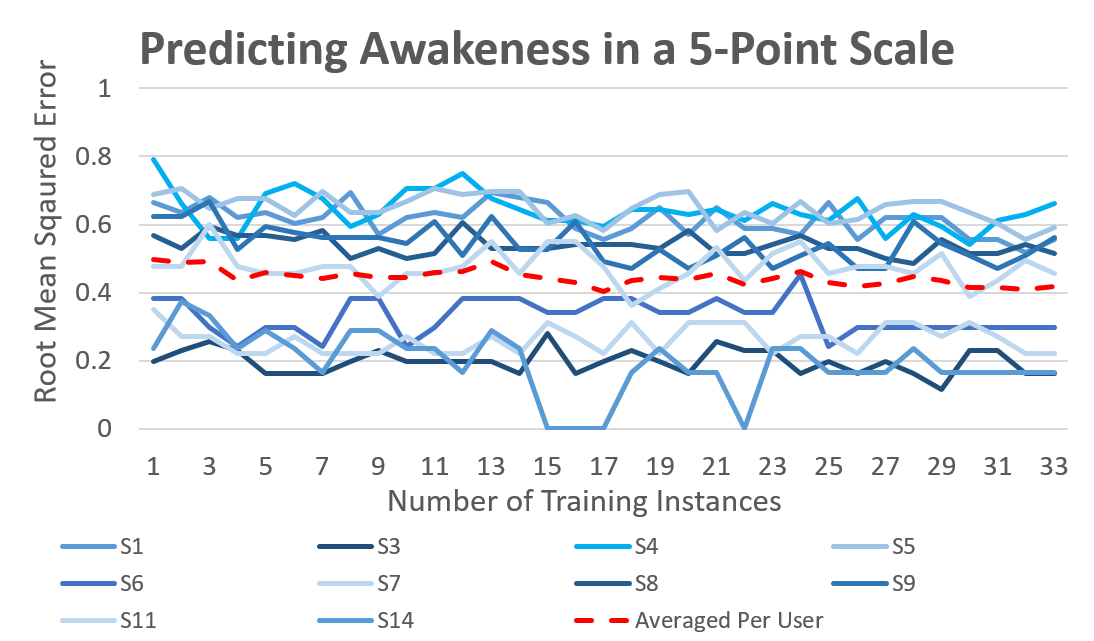
\includegraphics[width=0.5\textwidth]{20180914Awakeness5PointScaleOnly15Lines.png}
  \caption{Performance of the per participant trained classifiers for predicting 5-point awakeness, measured in root mean squared error.}
   \label{fig:learningCurve5}
\end{figure}

\noindent\textit{Predicting Five Classes}\\
In a second step, we analyzed a more fine-grained prediction using the initial 5-point Likert scale responses rather than the binarized ones as output measure. Figure~\ref{fig:learningCurve5} depicts the performance of the individually trained classifiers in terms of the root mean squared error. The root mean squared error represents the distance of the predicted from the actual value, which provides a more nuanced measure of the performance in the fine-grained prediction case. The figure shows a similar trend as for the binarized prediction, in that the root mean square error averaged over all ten participants decreases with more samples (from 0.49 to 0.41 root mean square error) and thus the performance increases. At the same time, the figure also shows that the performance results for the fine-grained prediction, again, vary substantially across participants.

\subsection{Minimum Time Window}\label{secMinimumTW}
In general, the less biometric data is needed to accurately predict a certain outcome measure, the easier and faster the analysis and data collection. To examine the optimal and minimum time window for the prediction of stress, focus, and awakeness, we used 16 different time windows from 10 seconds to 3 hours as depicted in Figure~\ref{timeWindows}. For our analysis, we then trained individual classifiers for each of the 16 time windows, using only features that had a time window smaller or equal to the time window rather than using all combinations of $\{Biometric Measures\} X \{Statistical Metrics\} X \{Time Windows\}$. We again used random forest and a leave-one-out cross validation to train individual classifiers. Since the number of features used for the training changed with each time window, we did not apply our feature selection in this case, but used all features available. Finally, due to the imbalance in the data, we again weighted each participants' classifier performance by the number of instances in the smaller class to calculate the average.

\begin{figure}
  \centering
      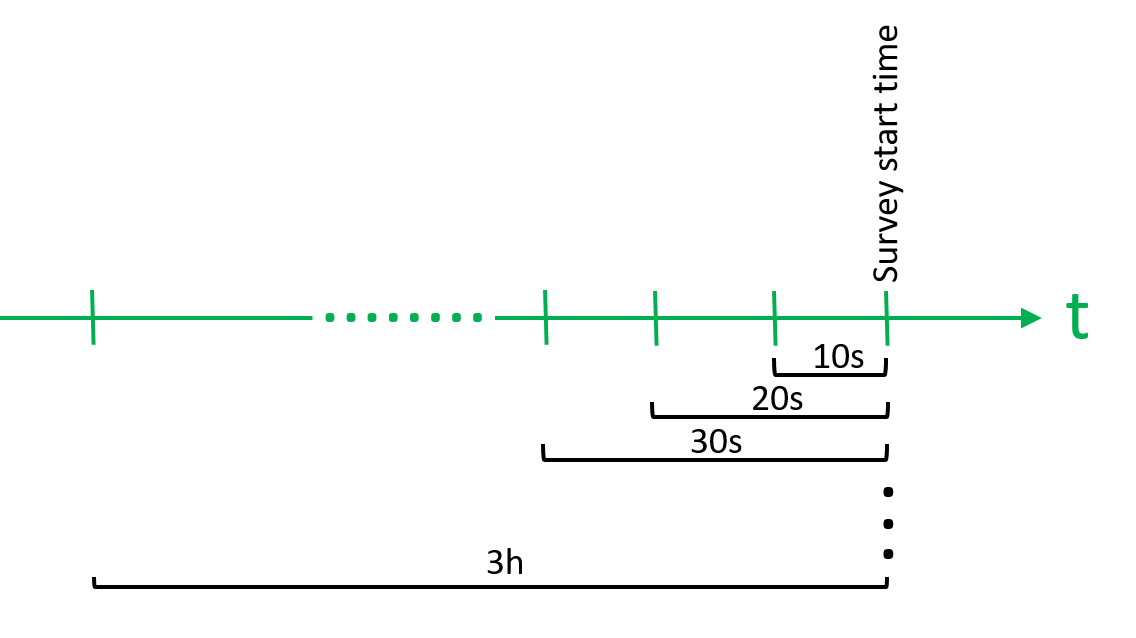
\includegraphics[width=0.4\textwidth]{timeWindows.png}
  \caption{Time windows of biometric data collected prior to each survey response: 10sec, 20sec, 30sec, 45sec, 1min, 2min, 3min, 5min, 7.5min, 10min, 20min, 30min, 45min, 1hour, 2hour, and 3hour.}
   \label{timeWindows}
\end{figure}

Figure~\ref{timeWindowsPandR} shows how the F-score changes for predicting 
`awake' over the 16 different time windows. The figure shows an increasing 
trend in the F-score, i.e. the higher the number of included time windows, 
the higher the F-score. However, there is one exception, the time window of 
1200 seconds that achieves a performance close to the one for the time 
window 10,800 seconds (3 hours), at which point all features are included. 
Overall, our results thus show that while using all time windows up to 3 
hours performs best, and outperforms the feature set that is solely based on 
a 10 second time window by 28\% (from 0.18 to 0.24), the performance for a 
time window of 1200 seconds is a good trade-off for selecting a shorter time 
window while maintaining high performance.

\begin{figure}
  \centering
      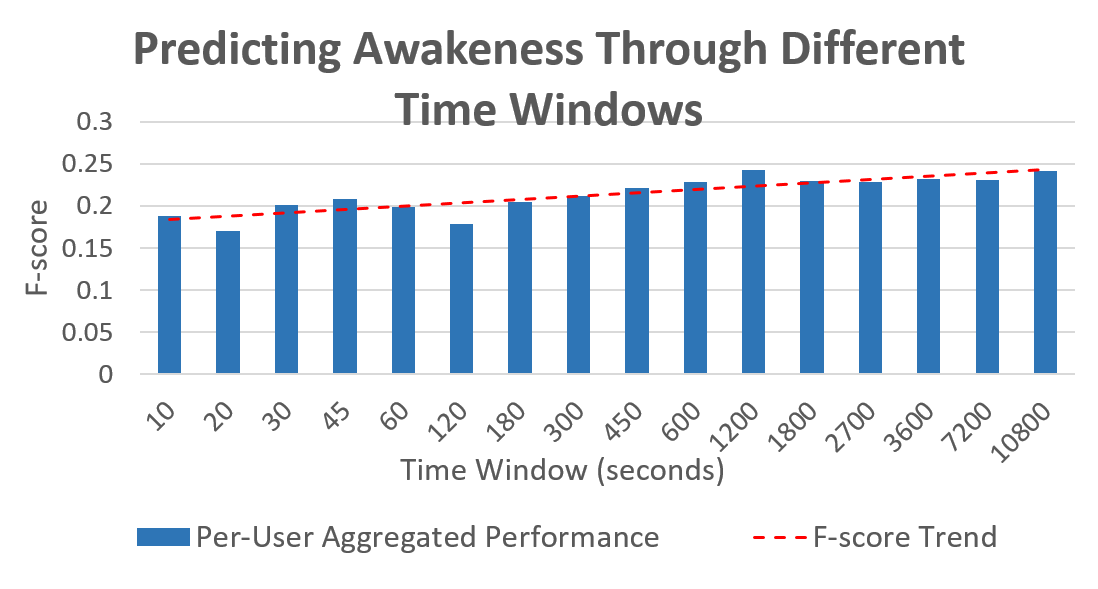
\includegraphics[width=0.5\textwidth]{20180912AwakenessTWBars.png}
  \caption{Performance (F-score) of individual classifiers trained on the different time windows to predict `awake'.}
  \label{timeWindowsPandR}
 % \vspace*{-3mm}
\end{figure}

%We also compared the performance of a model created per user against
%a model created across users.
%To calculate the performance of the model created per user,
%for each user we create a model using the features 
%related to each time window for the selected user only, 
%while in the model created with data across users,
%we trained the model with the data related to each
%particular time window of all users.
%our results show that the personalized model created
%for each user outperforms in every case
%the model created the with data across all users.

%This study
%shows that in general larger time windows predict stress,
%focus, and awakeness more precisely than 
%shorter time windows. We can also notice
%a very gentle upwards trend
%with a inflexion points at 45 seconds and 180.
%There is a peak of performance in 45 seconds, 
%time window that could be used if time is a scarce resource.
%The performance stabilizes around 180 time window
%which indicates that collecting data for a longer time
%period will not increase significantly the performance of the approach.
%The difference in performance between the 
%lowest performing and the highest performing time window is 
%less than a 10\% improvement. 


\subsection{Computer Interaction Data} \label{secCI}
Given our focus on knowledge workers (i.e., workers who generally spend a lot of time interacting with information on their computer at work), we also analyzed the use of computer interaction features to predict focus, awakeness and stress. To collect computer interaction data, we used an open source computer interaction monitor (reference omitted for double-blind.)
%the open source PersonalAnalytics project\footnote{https://github.com/sealuzh/PersonalAnalytics}  \cite{meyer18} 
to track participant's mouse and keyboard activity, as well as details about their active window. The specifics of the features tracked are listed in Table \ref{tracker}. The tracker was installed on the computers of 10 of the 14 participants, with participants S6, S10, S12, and S13 opting out of this part of the study due to privacy concerns.  Therefore, we limited this analysis to the 10 participants for whom we could calculate all features. 

\begin{table}
\begin{center}
\small\addtolength{\tabcolsep}{-1pt}
\begin{tabular}{l l}
\hline

Feature collected by tool & Description \\ 
\hline
Total keystrokes per min& Sum of all types of keystrokes \\ 
Normal keystrokes per min&F[h] Not backspace and navigation \\ 
Backspace keystrokes per min& Backspace keystrokes \\ 
Navigation keystrokes per min& Arrow key keystrokes \\ 
Total clicks per min& Sum of all click types \\ 
Other clicks per min& Not right and left clicks \\ 
Left clicks per min& Left clicks \\ 
Right clicks per min& Right clicks \\ 
Scrolled distance per min& Scrolled distance in pixels \\ 
Moved distance per min& Mouse movements in pixels \\ 
Activity switches per min& Browser window title changes \\ 
Category switches per min& Activity performed category \\ 
\hline
\end{tabular}
\caption{Features collected per user by the computer interaction tracker}%~\cite{meyer18}}
\label{tracker}
\end{center}
%\vspace*{-1mm}
\end{table}

For calculating computer interaction features, we again used the aforementioned 16 time windows and scaled the computer interaction values if the time windows did not align. For our comparative analysis of the different sensing techniques---biometrics vs computer interaction---we then created two new feature sets for each participant in addition to the biometric one: one with only computer interaction features, and one with computer interaction features plus biometric features. 

Table~\ref{ciPerformance} lists the results of our analysis. The results show that in all cases, the computer interaction based model was able to improve upon the biometric model in terms of precision and recall.
%MS is removing the accuracy results because it is not what we care about and it is just making the results harder to understand
%, but not in accuracy. 
Further, we found that the combined model was the most effective model in terms of precision and recall for predicting stress and awakeness overall, but performed slightly worse than the model using only computer interaction features for focus. 
%Since we consider precision and recall for predicting the class of higher interest, i.e. stressed, not focused, not awake, to be the most important statistics when interpreting our results, we compared the models against each other by averaging these two statistics.


\begin{table}
\begin{center}
%\small\addtolength{\tabcolsep}{-1pt}
\begin{tabular}{llllll}
\hline
Model/Feature Set & Precision & Recall & F-Score \\ %& Accuracy\\
\hline
\textbf{Awakeness}\\
\hspace{3mm}Biometrics only  & 0.269 & 0.314 & 0.289 \\ %& 0.808\\
\hspace{3mm}C.I. only  & 0.425 & 0.362 & 0.391 \\ % & 0.758\\
\hspace{3mm}Biometrics + C.I. & 0.390 & 0.404 & 0.400 \\ % & 0.791 \\
\hline
\textbf{Stress}\\
\hspace{3mm}Biometrics only  & 0.270 &	0.260 & 0.265 \\ % & 0.775\\
\hspace{3mm}C.I. only & 0.290 & 0.272 & 0.281 \\ % & 0.698 \\
\hspace{3mm}Biometrics + C.I. & 0.317 & 0.286 & 0.301 \\ % & 0.712\\
\hline
\textbf{Focus}\\
\hspace{3mm}Biometrics only & 0.251 & 0.256 & 0.253 \\ % & 0.716\\
\hspace{3mm}C.I. only & 0.332 & 0.342 & 0.337 \\ % & 0.742\\
\hspace{3mm}Biometrics + C.I. & 0.340 & 0.316 & 0.328 \\ % & 0.745\\
\hline
\end{tabular}
\caption{Comparison of the performance of predicting stress, focus and awakeness using the 3 different feature sets for the 10 participants. The performance is calculated as the average of the performance of the individual classifiers. Computer Interactions is abbreviated as C.I. here for readability. Precision and recall refer to the prediction of the more important classes, i.e. `stressed', `not awake', `not focused'.}
\label{ciPerformance}
\end{center}
%\vspace*{-1mm}
\end{table}

As with the biometric models, the individual performance of both the computer interaction only models and the combined models varied quite a bit between participants. Using stress as an example again, in the computer interaction models 5 of the 10 participants saw improvements compared to the baseline, with a maximum improvement of 128\% in precision, and 78\% in recall. In the combined model for stress, 5 of the 10 participants saw improvements compared to the baseline, with a maximum improvement of 117\% in precision and 95\% in recall. Neither model was capable of correctly predicting any instances of 'stressed' for participant S7.

Since the number of features changes  depending on which feature set is used, we adjusted the feature selection parameter for each of the computer interaction and combined computer interaction/biometric models. The values reported in this section were achieved using the optimal feature selection parameters we found, which are shown in Table \ref{ciFeatureSelection}.

\begin{table}
\begin{center}
\begin{tabular}{lc}
\hline
Model/Feature Set & Number of Features Selected\\
\hline
\textbf{Stress}\\
\hspace{3mm}C.I. & 400\\
\hspace{3mm}Biometrics + C.I. & 800\\
\hline
\textbf{Focus}\\
\hspace{3mm}C.I. & 20\\
\hspace{3mm}Biometrics + C.I. & 300\\
\hline
\textbf{Awakeness}\\
\hspace{3mm}C.I. & All\\
\hspace{3mm}Biometrics + C.I. & 50\\
\hline
\end{tabular}
\caption{The optimal number of features we found to select for each of the model/feature set combinations. Computer interactions is abbreviated as C.I.}
\label{ciFeatureSelection}
\end{center}
\vspace*{-4mm}
\end{table}



%\section{Analysis and Results}

%% To evaluate the efficacy of continuously predicting a knowledge worker's stress, focus, and awakeness in the workplace, we trained and tested machine learning classifiers using a leave-one-out cross validation. For prediction, we used the features extracted from the collected data as the input data, and binarized the participants' self-reported responses on stress, focus, and awakeness into two classes each (e.g., 'stressed' and 'not stressed') to use as output measures.

\section{Observed Trends Over Time in Stress and Awakeness Levels}
\label{stressTrends}

To gain insights into how knowledge workers experience stress and awakeness over an
extended period of work, we examined the end of day survey responses
collected from each participant to see if any identifiable trends
emerged. As we noted in the last section, we did not ask
participants about focus in the end of  day surveys as focus is an 
aspect relevant at a particular moment in time rather than an aspect
for an extended period of work. We used data from 13 of the 14 participants - we excluded one participant
from this analysis as they experienced atypical stress
levels in the latter half of the study due to factors outside of our
control.

\subsection{Stress Levels}
Overall, we identified three prominent characteristics in the stress levels.
%\rev{We describe characteristics noted in the reporting of the knowledge workers about the stress they experienced over the duration of the study.}

\begin{figure}[h!]
  \centering
      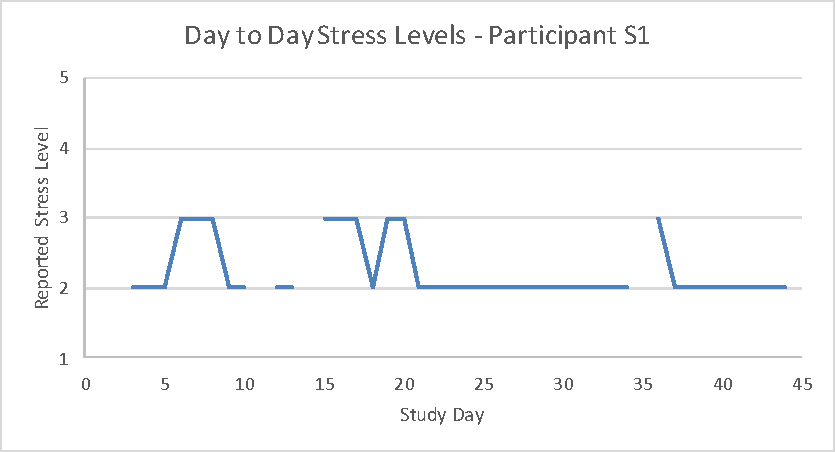
\includegraphics[width=0.7\textwidth]{s1_stress.pdf}
      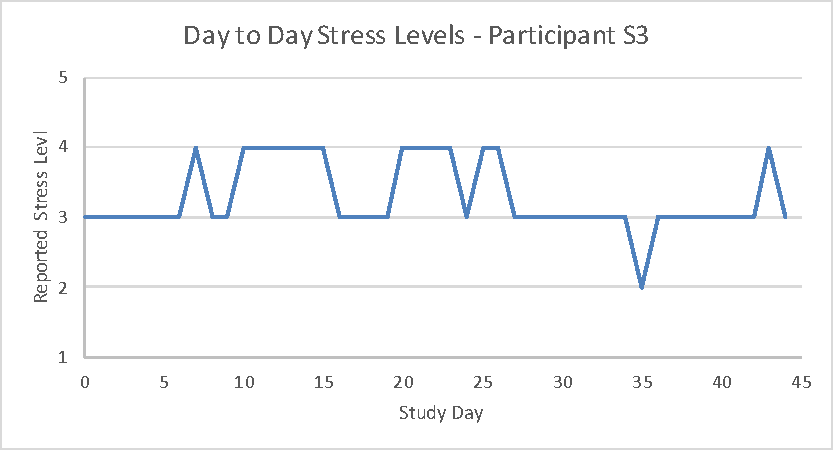
\includegraphics[width=0.7\textwidth]{s3_stress.pdf}
  \caption{The day-to-day stress levels reported by two participants (S1 and S3) are shown. The y-axis represents values on the 5-point Likert scale we asked participants to respond with ranging from 1/Not at all stressed to 5/Extremely stressed. The x-axis represents the day of the study on which the value was recorded (from 0-45). Some gaps are present in the chart for S1 as they did not report their stress level on those days.}
   \vspace*{-2mm}
   \label{fig:dailyStress}
\end{figure}


\subsubsection{Baseline Stress Levels}
%\noindent\textit{\textbf{Baseline Stress Levels.}}
Common amongst all participants was a trend to select one stress rating
far more frequently than any other. We will refer to this value as the
participant's baseline stress level. All but one participant reported
their perceived stress level for the day as their baseline stress
level more than 50\% of the time. In total, the baseline values made
up 65\% of the reported values collected from
participants. Interestingly, while participants sometimes saw periods
of sustained increases in stress, lasting as many as 6 consecutive
workdays in the most extreme case, participants would always return to
their baseline stress level at some point.


The baseline stress level varied significantly between participants. \rev{Seven}
participants (54\%) reported feeling average stress levels most frequently
(rating 3 on our scale), while \rev{five} (38\%) reported feeling little stress
(rating 2) and \rev{one} (8\%) reported feeling no stress at all (rating 1). Figure \ref{fig:dailyStress} illustrates these points using  data from two participants, showing the tendency to report and return to baseline stress levels, as well
as a distinct difference in baseline stress level (rating 2 for S1 vs rating 3 for S3). Gaps in the chart for S1 represent days for which the participant did not report their stress level.


\subsubsection{Stressful Days Tend to Cluster}
Accounting for the variance between participants perceived stress
baselines, we consider a stressful day to be one that represents a
deviation of \rev{one} or more stress levels above the participant's
baseline. Of the 93 stressful days we observed in total, we found that
39 (41\%) of these days occurred in groupings of two or more
consecutive stressful workdays. The most common size of these groups
was two workdays, while the largest group we observed was six
workdays.  The day after a stressful day is much more likely to be a
stressful day as compared to any other day with a 0.55 average increase
over baseline, compared to 0.02 average increase over baseline.

\subsubsection{Extreme Changes in Stress Levels are Rare}
After accounting for each participant's perceived stress baseline, we
examined the frequency of deviations from the baseline. We found that
participants were far more likely to report a stress level that was
within \rev{one} point of their baseline, than to report a stress level 2 or
more points away. These extreme deviations represented only 15\% of
all reported values, which differed from the \rev{participant's} baseline. As
well, the majority (78\%) of these deviations came from just two
participants. This suggests that some people may be less resilient to
the stress of the workplace than others. For most participants,
extremely stressful days were few and far between.

\subsection{Awakeness}
We applied the same analyses described above to the \rev{self-reported} awakeness levels of our participants. Compared with the reported stress levels, we observed the same trend of participants reporting one baseline far more commonly than any other. We did not find there to be a significant correlation between reported stress and awakeness levels. Overall, \rev{participant's} awakeness levels fluctuated significantly less than their stress levels (73.1\% of reports were at the baseline level, compared to 65.1\% for stress, p < 0.05). Participants were unlikely to experience days with heightened (above baseline) awakeness. Such days made up only 6.0\% of the total observed \rev{workdays} across all participant. Most of these days came from one participant, S2, who reported 15 heightened awakeness days compared to the next highest, S13 with four. Large deviations (>1 point deviation) from each participants baseline awakeness levels were extremely uncommon, accounting for only \rev{nine} (2.1\%) of our total observations. Similarly to what we observed with high stress days, low awakeness days frequently came in clusters of two or three days in a row. Given that the immediately preceding day was a low awakeness day\rev{;} a given day was 228.2\% more likely to be a low awakeness day than when considering any day at random (p < 0.0001).


\begin{table}[]
    \centering
\rev{\begin{tabularx}{\textwidth}{|c|c c c|c c c|}
    \hline
        &
        \multicolumn{3}{c|}{Stress} & 
        \multicolumn{3}{c|}{Awakeness} \\
        \hline
        \textbf{Variable} & \centering
        \textbf{\rev{F.E.E.}}& \textbf{p-value} & \textbf{\rev{C.I. (95\%)}} & \centering \textbf{\rev{F.E.E.}}  & \textbf{p-value} & \textbf{\rev{C.I. (95\%)}}\\
        \hline
        Monday & \centering -0.033 & 0.745 & \rev{$(-0.234, 0.167)$} & \centering -0.058 & 0.497 & \rev{$(-0.227, 0.110)$}\\
        Tuesday & \centering 0.028 & 0.773 & \rev{$(-0.164, 0.221)$} & \centering 0.036 & 0.662 & \rev{$(-0.126, 0.198)$}\\
        Wednesday & \centering 0.163 & 0.100 & \rev{$(-0.031, 0.357)$} & \centering -0.018 & 0.830 & \rev{$(-0.181, 0.145)$}\\
        Thursday & \centering 0.022 & 0.821 & \rev{$(-0.169, 0.213)$} & \centering 0.076 & 0.927 & \rev{$(-0.085, 0.238)$}\\
        Friday & \centering 0.082 & 0.473 & \rev{$(-0.142, 0.306)$} & \centering -0.178 & 0.025 & \rev{$(-0.334, -0.022)$}\\
        Month End & \centering 0.044 & 0.687 & \rev{$(-0.171, 0.259)$} & \centering -0.082 & 0.374 & \rev{$(-0.263, 0.099)$}\\
        \hline
    \end{tabularx}
    \caption{\rev{Fixed effects estimates (F.E.E.), 95\% confidence intervals and associated p-values for the explanatory variables (day of week and proximity to month end) that we examined in our linear mixed model analysis.}}    \label{tab:mixedModel}}
\end{table}





\subsection{Explaining Fluctuations}
In an attempt to explain some of the fluctuations in stress and awakeness that our participants were experiencing, we created a linear mixed model with the self-reported daily stress and awakeness levels as dependent variables and the participants as random effects. We experimented with day of the week and proximity to beginning or end of month as possible explanatory variables. Ultimately, the analysis showed that none of the variables that we examined had a significant explanatory power with respect to our participants perceived stress levels.
For awakeness, we found  that there was a small (\rev{fixed effects estimate}: -0.178) yet significant decrease in awakeness levels on Fridays in particular. Table \ref{tab:mixedModel} shows some of the detailed results of these analyses. These results show the difficulty of explaining a person's stress and awakeness via simple measures, and point to the need for additional instrumentation and data collection if we are to successfully understand and make predictions about these human aspects in the workplace.




\section{Predicting Stress, Focus and Awakeness in the Moment}
% random forest best
\label{secOverallAccuracy}

To investigate whether stress, focus and awakeness can be predicted in
the moment based on biometric measures,
we investigated classifiers trained
for each individual and across all participants. We report on the effectiveness of
these classifiers and the features that are important in predicting stress, focus
and awakeness.

\subsection{Data Preparation}

\rev{In a machine learning context, data preparation and utilization is an essential part of the proposed solution. To prepare} the collected data for use in training and testing \rev{our proposed} machine learning models, we performed \rev{the following} steps.


\subsubsection{Data Cleaning}
All data recorded by the Everion is associated with a quality score ranging from 0-1 that is calculated using proprietary methods. In accordance with the recommendations of Biovotion,
to prevent our results from being effected by erroneous data we set a quality threshold of 0.5 and discarded any data gathered which had a quality rating below this threshold. 

\subsubsection{Data Linking}

We linked the collected biometric data and survey responses for each participant. Linking the data is necessary to construct training and test datasets for use in creating and evaluating machine learning models.

To link the data, we look back one hour from the start time of each survey response for
available biometric data.  For example, if a participant started a survey response at 11:05am, we look for biometric data from between 10:05am to 11:05am. If no biometric data was recorded in the hour time window, we exclude the survey response from the dataset. Otherwise, we consider the survey response to have associated biometric data.

There are several reasons for a survey response to lack associated biometric data:
\begin{itemize}
\item The participant was not wearing the Everion in the hour before beginning the survey.
\item The Everion was not recording data in the hour before the participant began the survey (e.g., due to low battery).
\item Biometric data was not being uploaded successfully to the server.
%\item Compatibility issues between the sensor and the OS tracking the participant's data
%\item Issues accessing the data uploaded by the participants
\end{itemize}

Figure~\ref{surveyBio} illustrates the number of survey responses with associated biometric data for each study participant. 
%This was added to address REviewer 2's concern: Is it correct that the maximum number of responses should have been 112 on the surveys?
The total number of responses per participant is affected by their response rate and by the number days out-of-office (e.g., vacations, holidays, etc.). 
Participant S2 and S12 have particularly low numbers of usable survey responses. In each of these cases, the issue related to biometric data not being uploaded successfully to the server.

\begin{figure}
  \centering
      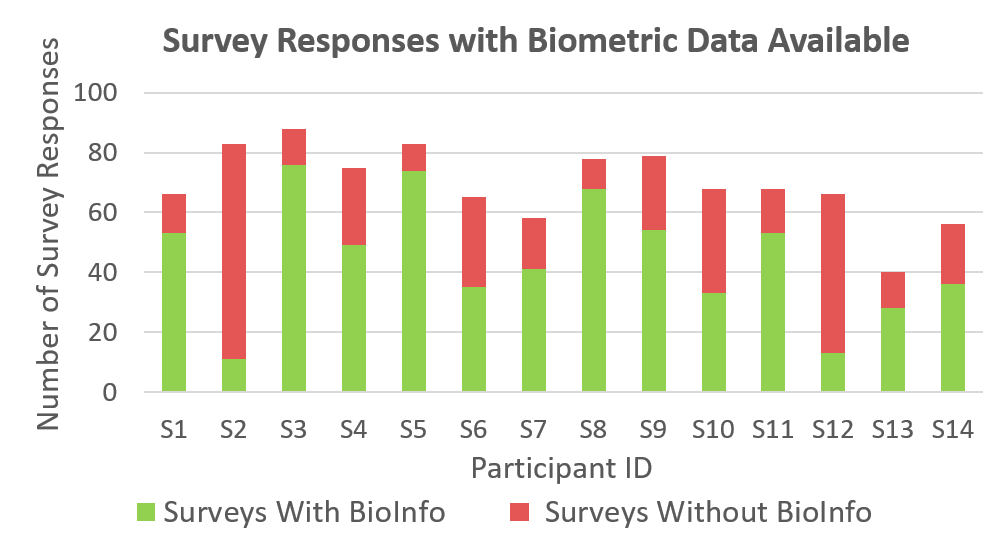
\includegraphics[width=0.8\textwidth]{DuringTheDay.png}
  \caption{The figure shows the biometric data available per each participant. Green sections represent survey responses with biometric
  data available, red sections responses with no biometric data available}
   \label{surveyBio}
   \vspace*{-4mm}
\end{figure}


\subsubsection{Feature Extraction}
We extracted features from the biometric data to provide as input to machine 
learning models. Previous 
studies~ \cite{vorburger05,zuger2015interruptibility} identify time windows as an 
important factor that impacts the prediction accuracy of a classifier. We 
considered many time windows from the literature on biometric 
analysis~\cite{zuger18}, ranging from 10 seconds to 3 hours. Specifically, we 
considered the following time windows: \textit{10sec, 20sec, 30sec, 45sec, 
1min, 2min, 3min, 5min, 7.5min, 10min, 20min, 30min, 45min, 1hour, 2hour, 
3hour}.

From the start time of each survey response, we look back the amount of time 
that corresponds to each time window and we create features for all of the 
biometric data available in that time window. For example, if a participant 
started a survey response at 11:05am, for the 30min time window, we create 
features using all of the available biometric data from 10:35am to 11:05am. 
If there is a large portion ($\geq$50\%) of data missing (either because of a recording issue or because of low quality data) from the time window considered, then the time window is marked as missing. In this case, features are imputed based on the mean of other samples of the same feature for that participant. This is an effective and commonly used technique, which is preferable to the alternative of deletion as it preserves our already small sample size~\cite{hawthorne2005imputing}.
For each time window, we calculate 10 statistical measurements from the 
biometric data to create 10 distinct features. Specifically, the 10 
statistical measurements are: mean, standard deviation, variance, median, 
25\textsuperscript{th} percentile, 75\textsuperscript{th} percentile, interquartile range, maximum, minimum, and 
range. Thus, for each survey response, we generate a large number of 
corresponding features based on three factors: biometric measurement, time 
window, and statistical measurement. In addition to these biometric 
features, we also considered the time of day in which the questions were 
asked. These features are created to predict the responses described by the 
ground truth. To attempt to account for inter-participant differences, we normalized all features on a per-participant basis.

\begin{table}
  \centering
      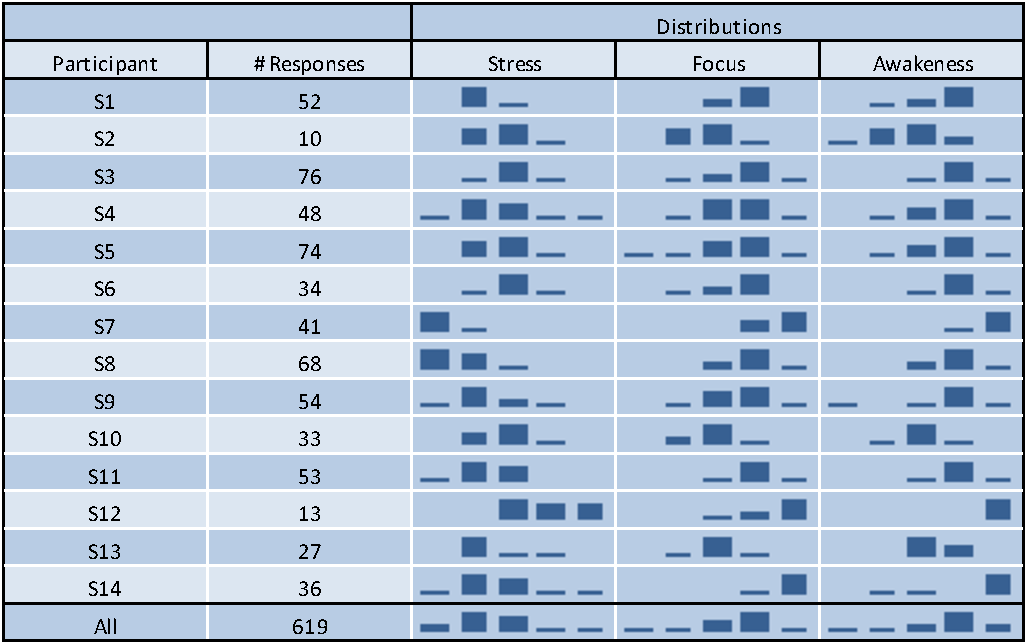
\includegraphics[width=0.8\textwidth]{distributiontable.pdf}
  \caption{The distribution of the responses of each participant to the three questions asked during the day are shown. Each bar in the histograms represent one of the \ref{five} values on the 5-point Likert scale we asked participants to respond with, where the far left side of the histograms are 1/Not at all, and the far right sides are 5/Extremely}
   \label{responseDistribution}
   %\vspace*{-2mm}
\end{table}

\subsubsection{Response Transformations}
Table~\ref{responseDistribution} illustrates the distribution of responses from each participant for each of the three survey questions (listed in Section~\ref{sec:Surveys}). The figure shows that there is a notable imbalance in the distribution of the self-reported responses provided by the participants. Most participants did not use all five points of the five-point Likert scale in their responses, and the distributions tend to skew toward one side or the other, depending on the question. Given 
this distribution and based on our earlier observation that the participants tended to adhere to a baseline reporting level for stress and awakeness, we elected to simplify the problem from \rev{five} classes to \rev{two}. This transformation enables us to more easily represent patterns in the data, such as when a participant fluctuates from a normal to high stress level. To perform this transformation, \rev{we began by calculating the median response value for each participant and each question}. We classified each response below the median as 0 (`negative') and each response above the median as 1 (`positive'). The distribution for the stress question skewed left, so we included the median values in the `positive' class (i.e. `stressed'), while the distributions for focus and awakeness skewed right, so we included those median values in the `negative' class (i.e. `not focused', `not awake').

With this method, we transformed the survey data into a two-point scale, representing  negative or positive responses for each of the three human aspects of interests (e.g., not stressed or stressed). 

\subsubsection{Oversampling}
Even after binarizing the responses as described in the previous section, we found the distribution of responses was still quite imbalanced for many of our participants. This can be seen in the distribution columns in Table \ref{tab:accuracy}. To mitigate this effect, we applied random oversampling to our training sets, which artificially rebalances the dataset by creating randomly replicated data in the minority class. This technique has commonly been used  in previous studies on unbalanced datasets \cite{chawla2004,yap2014}.

\begin{comment}
\begin{table}[h]
	\begin{centering}
	\small\addtolength{\tabcolsep}{-1pt}
    \begin{tabular}{llll}
      \hline
      Variable & K & \# Estimators & Minimum Samples Split \\
      \hline
      Stress & 300 & 100 & 4\\
      Focus & 200 & 50 & 4\\
      Awakeness & 800 & 100 & 4\\
      \hline
    \end{tabular}
    \caption{The hyperparameters selected by grid search analysis to tune our random forest models. K refers to the number of features selected.}    \label{tab:hyperparams}
    \end{centering}
\end{table}
\end{comment}


\subsection{Selecting a Classifier Algorithm}

\rev{Many different algorithms can be used to build a classifier.} To select an
algorithm, we compared multiple classifiers using the popular machine learning library scikit-learn~\cite{pedregosa11},  evaluating each one by using leave-one-out cross validation. Our analysis showed that random forest outperforms all other classifiers, including Na\"ive Bayes, decision trees, support vector machine, and a multilayer perceptron neural network. For the remainder of this paper, we refer to a random forest classifier.%\\[-0.1cm]
% for stress they were (minimum samples for split = 4, # of estimators = 100, max features = 0.5, k=300), for focus they were (minimum samples for split = 4, # of estimators = 50, max features = 0.5, k=200), and for awakeness they were (minimum samples for split = 4, # of estimators = 100, max features = 0.25, k=800)



\begin{table*}[h]
  \centering
  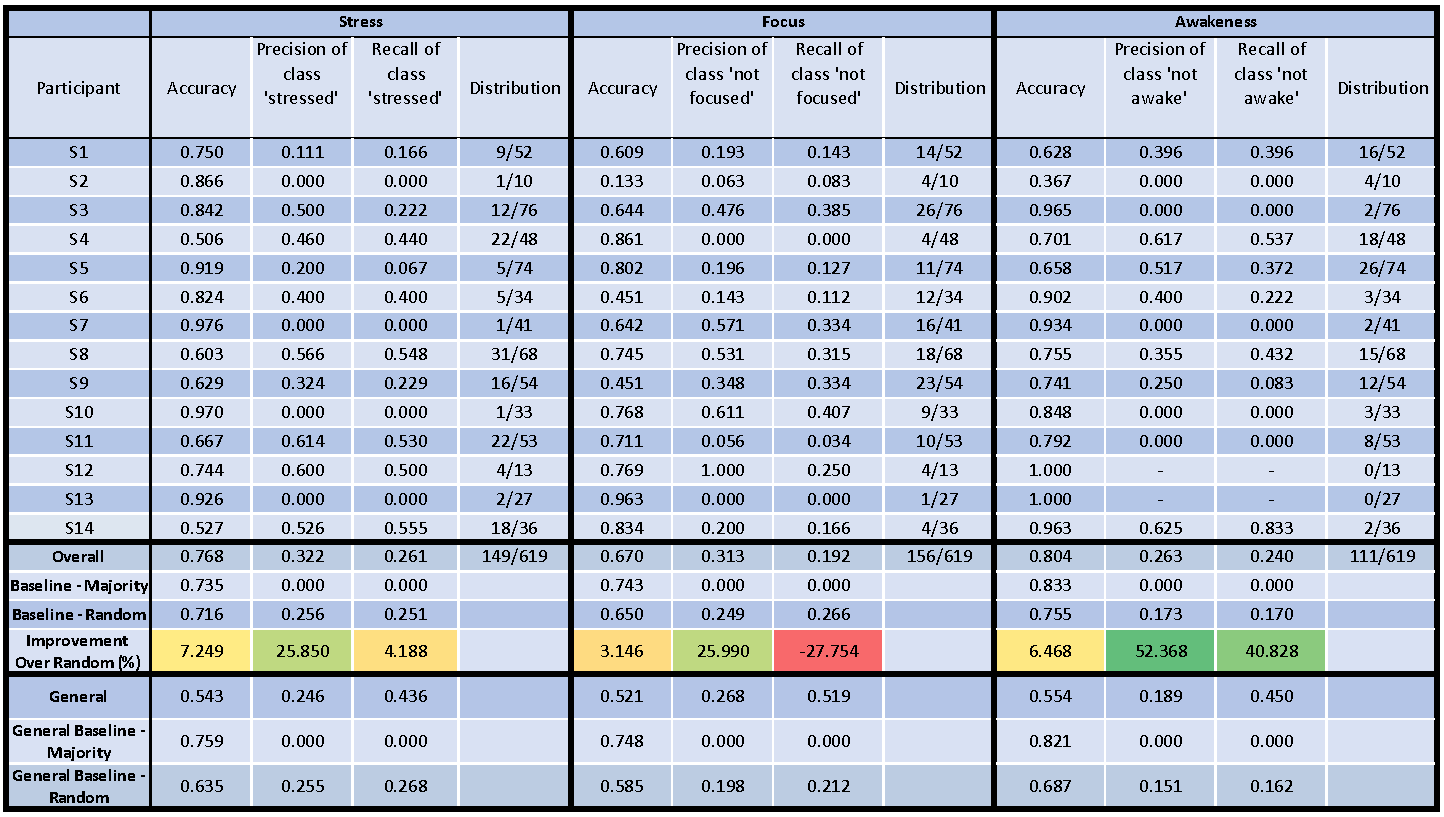
\includegraphics[width=1.0\textwidth]{rq1performance_v2.pdf}
  \caption{Results of predictions using the individual models. The distribution columns show the proportion of the minority class out of the total number of responses for each of the three variables. The baseline rows represents the averaged results of our baseline classifiers. The general row shows the averaged results of our models trained on all participants.}\label{tab:accuracy}%\todo{revise caption}}
  \vspace*{-4mm}
\end{table*}

\subsection{Individual Classifiers}
%\noindent\textit{Results of Individual Classifiers}\\
Since peoples' experience of stress, focus, and awakeness (as well as
their physiological manifestations) can vary substantially
(e.g.,~\cite{Hernandez11}), we first trained and evaluated individual classifiers
for each participant (as opposed to a general one for all
participants) using leave-one-out cross validation. The results of our analysis are reported in
Table~\ref{tab:accuracy}. For our analysis, we report values of
accuracy, one of the most commonly used metric to compare performance,
as well as precision and recall of the classes of interest:
`stressed', `not focused', and `not awake'. Since the imbalance in the
data can lead to high accuracy values if a classifier always just
predicts the most likely/frequent class while ignoring the class of
higher importance and interest, precision and recall of the class of
interest are also important to
consider~\cite{yap2014,bhattacharyya_data_2011,Hernandez11}.

\rev{Besides} our results, for the purposes of comparison\rev{,} we also present two commonly used baselines in this table - a majority classifier, which always predicts the larger of the two classes considered, and a stratified random classifier which randomly chooses between the two classes, but with a proportional bias towards the larger class.

For some users (i.e., S1. as seen in Table \ref{responseDistribution}), the imbalance in their data was so extreme that even after adjusting by oversampling\rev{, we were not able} to create a reasonable classifier. These scenarios are difficult to predict\rev{,} as any classifier will not have enough variance in its training data for the 'stressed' situation to adequately distinguish it from the non-stressed case.


% However, the imbalance in the data can lead to a classifier with high accuracy if it always just predicts the more likely class while ignoring the class of higher importance and interest in our case (i.e. stressed, not focused, not awake). Therefore, we further report the precision and recall for the three classes 'stressed', 'not focused' and 'not awake'. 


Overall, we were able to use extracted physiological features to
predict all three aspects with reasonable accuracy, precision, and
recall. We present a comparison between the averaged results of our individual classifiers and those of the baseline stratified random \rev{classifier} in the ``Improvement Over Random'' row of Table \ref{tab:accuracy}. This is calculated as the difference between the overall average and the baseline results, divided by the baseline results (for example, $\frac{Acc_{Overall} - Acc_{Random}}{Acc_{Random}}$). We do not compare our results with the majority classifier directly as this classifier achieved precision and recall scores of zero when predicting stress, lack of focus, and lack of awakeness, making a meaningful comparison \rev{unfeasible}. The improvement percentages demonstrate that the predictions made by our classifiers are much better than random after correcting for the imbalance in our dataset.

While the individually trained classifiers
improved on average across all participants upon the baseline in all
cases except in recall of `not focused', the improvement was
substantially higher for awakeness (52.4\% improvement in precision,
40.8\% in recall, and 6.5\% in accuracy) than for stress or focus. In addition,
the performance of the individually trained classifiers varied greatly
across participants. While some participants showed a large
improvement, for others the baseline performed much better than the
individually trained classifier. For instance, for predicting
`stressed', the individual classifiers improved upon the baseline for
S4, S6, S8, S11, S12, and S14 with a maximum improvement of 152.0\% in
precision and 111.1\% in recall for S12, while they did worse for S1,
S3, S5, S7, S9, S10, and S13, and in the worst cases did not correctly
predict a single instance of `stressed'. Typically, users that have the
lowest precision and recall values are those where the data is the
most imbalanced.\\[-0.1cm]
% We attribute these discrepancies to the large differences in response distributions between participants, as well as to the subjectivity of self-reporting.
%
%(improvement: 8\% precision, 1\% recall, 8\% accuracy), the individual performance varied greatly among participants. Some participants showed negligible difference in comparison to the baseline classifier, e.g. subject ..., while others showed a large improvement, e.g. subject ...
%\begin{table}[h!]
%\begin{centering}
%\begin{tabular}{lll}
%\hline
%Participant & Recall Improvement (\%) & Precision Improvement (\%)\\
%\hline
%S12 & 184.6 & 88.4 \\
%S6 & 66.7 & 85.8 \\
%S11 & 50.0 & 44.4 \\
%S8 & 32.4 & 26.7 \\
%S14 & 14.7 & 9.8 \\
%S4 & 5.6 & 5.5 \\
%S9 & -55.4 & -46.8 \\
%S3 & -90.0 & -82.1 \\
%S1 & -100.0 & -100.0 \\
%S5 & -100.0 & -100.0 \\
%S7 & -100.0 & -100.0 \\
%S10 & -100.0 & -100.0 \\
%S13 & -100.0 & -100.0\\
%S2 & - & -\\
%\hline
%\end{tabular}
%\caption{Percentage improvement in recall and precision for stress, using our approach compared to the baseline, on an individual level. For participant 2, the baseline achieved a precision and recall of 0, thus the improvement is undefined}
%\end{centering}
%\label{tab:indImprovement}
%\end{table}


\subsection{Feature Selection and Importance}
%\noindent\textit{Feature Selection and Importance}\\
There are a large variety of features that can be (and have been) calculated in previous research for each of the basic measurements listed in Table~\ref{signals}, such as the mean, standard deviation, maximum, and interquartile range. In addition, each of these metrics can be combined with the various time windows captured of a basic measurement, resulting in a large feature space. To reduce the feature space, we experimented with multiple feature selection methods, including selecting the top k highest correlated features by various metrics such as mutual information, Pearson's correlation coefficient, ANOVA's F-value, as well as wrapper methods such as recursive feature elimination, optimizing mean decrease accuracy by iteratively permuting features, and only selecting features that exceed a certain Gini importance threshold. We found that all methods produced similar results with respect to accuracy, precision, and recall for the individual models. Ultimately, we elected not to utilize any feature selection in order to simplify our approach, as we found there to be minimal differences in performance between the techniques, and the random forest algorithm is capable of (and robust for) handling datasets with many features.

%Respiration rate is also highly important for stress (#3 , 14.4%) but I'm not sure what previous works say about correlation with stress
Overall, the features that were selected as the important ones for the individual models based on the random forest algorithm varied greatly across participants. Yet, some feature categories were considered to be important more frequently than others. Table~\ref{tab:featureImportance} shows the averaged Gini importance for the feature categories used for predicting stress. Heart rate variability proved to be an important measure for all of the aspects of interest, ranking as the most important feature category for both stress and awakeness, and the second most important one for focus. This is not surprising, as heart rate variability and skin temperature have been shown in several previous studies to be possible indicators for stress levels~\cite{dishman2000stress,mcduff16,kataoka00}. We also found blood pulse wave to be an important indicator for both focus and awakeness, but less important for stress, while respiration rate was important in stress and focus but not awakeness. Besides these mentioned feature categories, there was great variation in which measures were important to which of the three aspects. This shows that there is a clear benefit to having multiple biometric streams available for predicting stress, focus and awakeness.\\[-0.1cm]


\begin{table}[h!]
  \begin{centering}
  \begin{tabular}{llll}
    \hline
    Feature Category & Stress & Focus & Awakeness\\
    \hline
    Heart Rate Variability & 18.3\% & 13\% & 13.6\%\\
    Blood Pulse Wave & 10\% & 14.2\% & 13.1\%\\
    Heart Rate & 8.7\% & 12.6\% & 10.3\%\\
    Skin Temperature & 15.7\% & 9.8\% & 10\%\\
    Galvanic Skin Response & 6.6\% & 8.2\% & 5.1\%\\
    Respiration Rate & 14.8\% & 12.7\% & 10\%\\
    Oxygen Saturation & 5.6\% & 4.3\% & 2\%\\ 
    Energy Expenditure & 6\% & 7.7\% & 4.8\%\\
    Activity & 4.6\% & 7.8\% & 7.6\%\\
    Steps & 1.7\% & 0.8\% & 0.9\%\\
    Time of Day & 0\% & 0.1\% & 0.5\%\\
    \hline
  \end{tabular}
  \caption{The averaged Gini importance of each feature category, per response variable.}
  \label{tab:featureImportance}
  \end{centering}
  \vspace*{-2mm}
\end{table}

\subsection{Individual vs.\ General Model}
%\noindent\textit{Individual vs.\ General Model}\\
Individual models are trained specifically for each individual and thus require a data collection period before they are capable of making accurate predictions. On the other hand, the idea of general models is to be able to train them on already collected data and then  to be able to apply them even to new and unseen individuals, thus overcoming the cold-start problem. Given the large individual differences in biometrics, training a general model to achieve an adequate accuracy for new individuals is not necessarily possible. 

To examine the performance of a general model for our participants, we trained three general models, one for focus, one for awakeness and one for stress. We roughly followed the same procedure as for the individual models. Due to the larger amount of data available in the general case, we used the more common random undersampling, which randomly selects elements in the majority class to exclude from the dataset, instead of random oversampling to balance the distribution of the dataset. The models were trained on the datasets of 13 of the 14 participants, and then evaluated on the dataset of the last (leave-one-participant-out cross-validation), repeating this process for all 14 participants. 

The bottom \rev{three} rows of Table \ref{tab:accuracy} present the averaged performance results for this approach in terms of accuracy, precision, and recall, as well as the results of baseline stratified random and majority classifiers following the same leave-one-group-out cross-validation procedure. Although the averaged precision and recall are comparable or better than those of the averaged individual results, this was at the cost of a large decrease in overall accuracy.  Upon closer investigation into the performance of the general model when testing on each participant, we found that individually trained models for each participant performed much better than a general model trained over all participants. Using stress as an example, for participant S12, for whom we saw the greatest increase compared to the baseline in individual models, the general model was unable to predict a single instance of `stressed' correctly. This is consistent with our expectations because biometric features are highly specific to individuals.


%\todo{put the content of the following sentence somewhere into the discussion; We attribute these discrepancies to the large differences in response distributions between participants, as well as to the subjectivity of self-reporting.}


%%!TEX root = bioPrediction_main.tex

\subsection{Minimum Number of Training Samples}\label{secLearningCurve}
Collecting experience samples from users is expensive, since participants 
are being interrupted several times a day and have to answer the survey. 
To minimize the number of samples to be collected from participants, we 
examined how the performance of individual classifiers changes over the 
number of samples used to train the classifier.

Participants in our study had varying levels of responsiveness to the 
experience sampling ranging from 10 to 76 (see Figure~
\ref{responseDistribution}).
%Answering Reviewer 2's concern: Why only 10 participants? What was the rationale for the cut-off selected? 
To answer this research question we analyze the maximum number of responses \textbf{all} analyzed participants have to train the model. Since some participants have a very small number of maximum answers (ten being the lowest) we excluded the four participants with the least number of responses for this analysis.
%To maintain a certain generalizability while 
%also being able to examine a range of sample numbers for training the 
%classifier, we removed the four participants with the least number of 
%samples for this analysis. 
As a result, we obtained a corpus of analysis where all participants have a 
higher number of responses (34 being the lowest), which allows us to examine 
the learning curve of the classifiers for a larger number of training data points. For our 
analysis, we thus performed a leave-one-out cross validation with random 
sample sets of size 1 to 33 and calculated the average through all folds of 
the validation.

For each of the three productivity-related aspects, we are again more 
interested in predicting when a worker is stressed, not awake, or not 
focused, the less common class in all three cases. Since the less common 
class can be very small, we weighted each participants' classifier 
performance by the percentage of the samples in this smaller class.

\begin{figure}
  \centering
          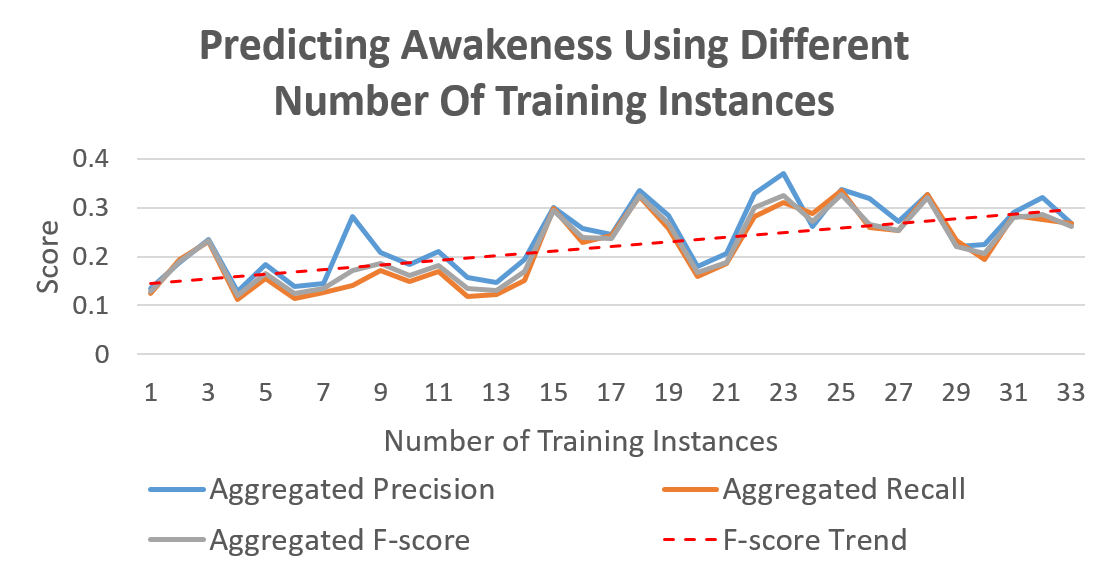
\includegraphics[width=0.5\textwidth]{20180912AwakenessLC2.png}
  \caption{Performance of the per participant trained awakeness classifiers, measured in precision, recall (sensitivity), and F-score. The dotted red line represents the F-score trend.}\label{fig:learningCurveInd}
  %\vspace*{-3mm}
\end{figure}

%\vspace{0.05in}
\noindent\textit{Individual Classifiers for Binary Prediction}\\
The averaged performance of all individually trained random forest classifiers for 'awake' with respect to the training sample size is presented in Figure~\ref{fig:learningCurveInd}. The trend indicates a positive correlation between the number of samples in the training set and the classifiers' F-score performance, with an overall improvement of  114\% (from 0.14 to 0.30) in the F-score between a training set of one sample to one with 33 samples. The trends for
the remaining indicators are 29\% for stress and no overall improvement for focus.%\\[-0.1cm]

%\noindent\textit{}
%When contrasting
%models trained and tested on the 
%biometric data of each user individually, against
%a general model trained and tested with the data of all users. 
%We can conclude
%that for up to 33 training samples analyzed in this study,
%the former has better performance when predicting the
%responses of each user than when training 
%a model with the data of several different users. 
%This is partially due to the 
%variability across users and the subjective nature
%of the responses (e.g.,where slightly awake for one person
%may be not awake for another). 

\begin{figure}
  \centering
      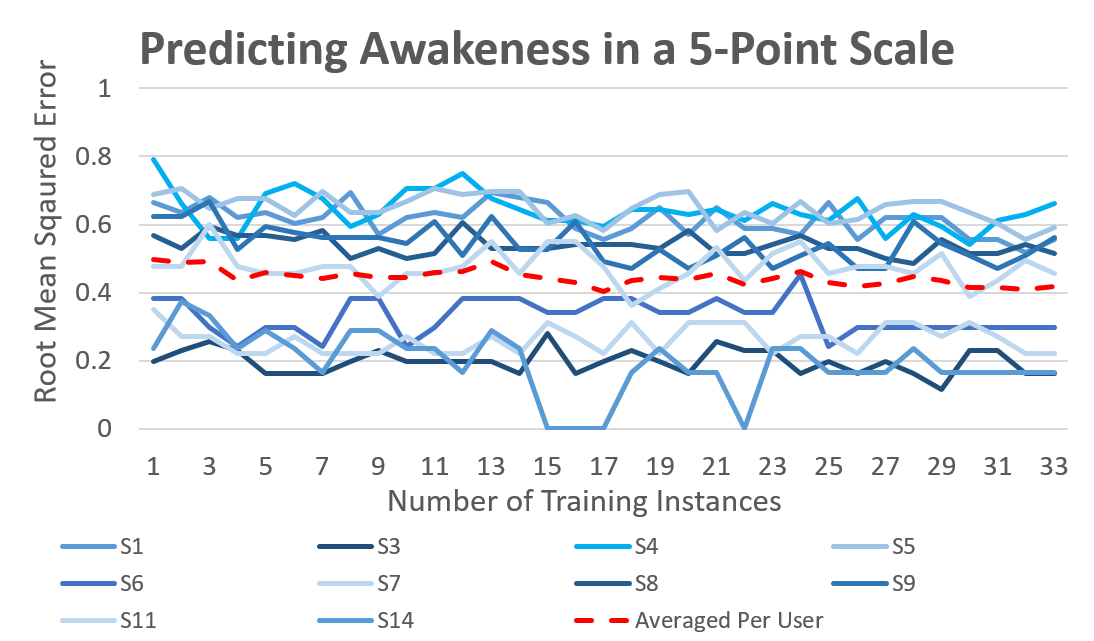
\includegraphics[width=0.5\textwidth]{20180914Awakeness5PointScaleOnly15Lines.png}
  \caption{Performance of the per participant trained classifiers for predicting 5-point awakeness, measured in root mean squared error.}
   \label{fig:learningCurve5}
\end{figure}

\noindent\textit{Predicting Five Classes}\\
In a second step, we analyzed a more fine-grained prediction using the initial 5-point Likert scale responses rather than the binarized ones as output measure. Figure~\ref{fig:learningCurve5} depicts the performance of the individually trained classifiers in terms of the root mean squared error. The root mean squared error represents the distance of the predicted from the actual value, which provides a more nuanced measure of the performance in the fine-grained prediction case. The figure shows a similar trend as for the binarized prediction, in that the root mean square error averaged over all ten participants decreases with more samples (from 0.49 to 0.41 root mean square error) and thus the performance increases. At the same time, the figure also shows that the performance results for the fine-grained prediction, again, vary substantially across participants.

\subsection{Minimum Time Window}\label{secMinimumTW}
In general, the less biometric data is needed to accurately predict a certain outcome measure, the easier and faster the analysis and data collection. To examine the optimal and minimum time window for the prediction of stress, focus, and awakeness, we used 16 different time windows from 10 seconds to 3 hours as depicted in Figure~\ref{timeWindows}. For our analysis, we then trained individual classifiers for each of the 16 time windows, using only features that had a time window smaller or equal to the time window rather than using all combinations of $\{Biometric Measures\} X \{Statistical Metrics\} X \{Time Windows\}$. We again used random forest and a leave-one-out cross validation to train individual classifiers. Since the number of features used for the training changed with each time window, we did not apply our feature selection in this case, but used all features available. Finally, due to the imbalance in the data, we again weighted each participants' classifier performance by the number of instances in the smaller class to calculate the average.

\begin{figure}
  \centering
      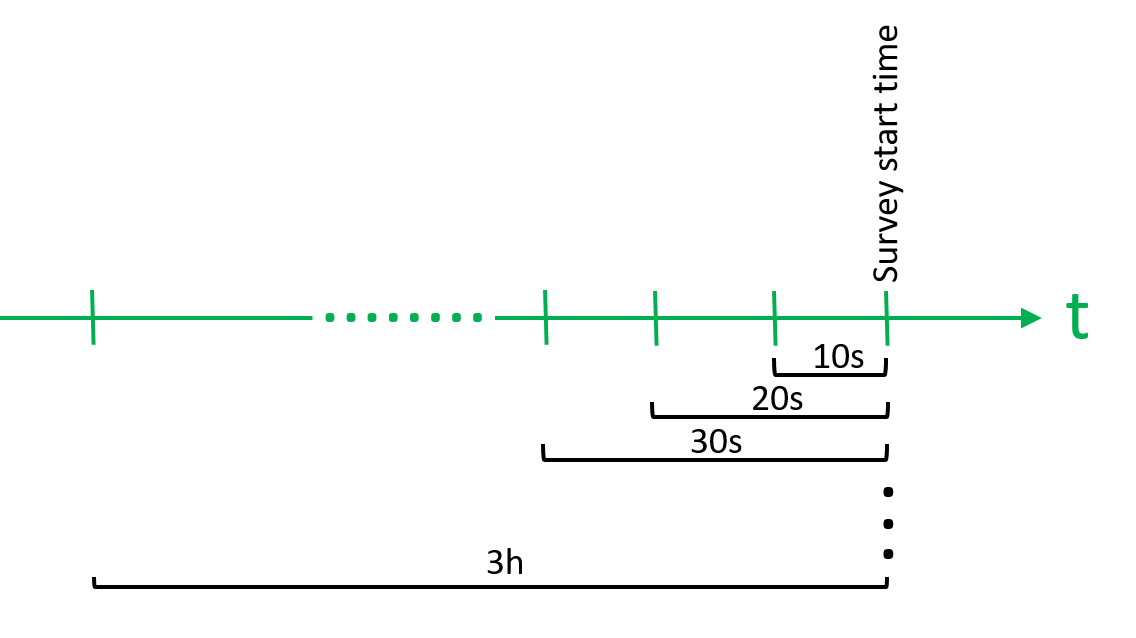
\includegraphics[width=0.4\textwidth]{timeWindows.png}
  \caption{Time windows of biometric data collected prior to each survey response: 10sec, 20sec, 30sec, 45sec, 1min, 2min, 3min, 5min, 7.5min, 10min, 20min, 30min, 45min, 1hour, 2hour, and 3hour.}
   \label{timeWindows}
\end{figure}

Figure~\ref{timeWindowsPandR} shows how the F-score changes for predicting 
`awake' over the 16 different time windows. The figure shows an increasing 
trend in the F-score, i.e. the higher the number of included time windows, 
the higher the F-score. However, there is one exception, the time window of 
1200 seconds that achieves a performance close to the one for the time 
window 10,800 seconds (3 hours), at which point all features are included. 
Overall, our results thus show that while using all time windows up to 3 
hours performs best, and outperforms the feature set that is solely based on 
a 10 second time window by 28\% (from 0.18 to 0.24), the performance for a 
time window of 1200 seconds is a good trade-off for selecting a shorter time 
window while maintaining high performance.

\begin{figure}
  \centering
      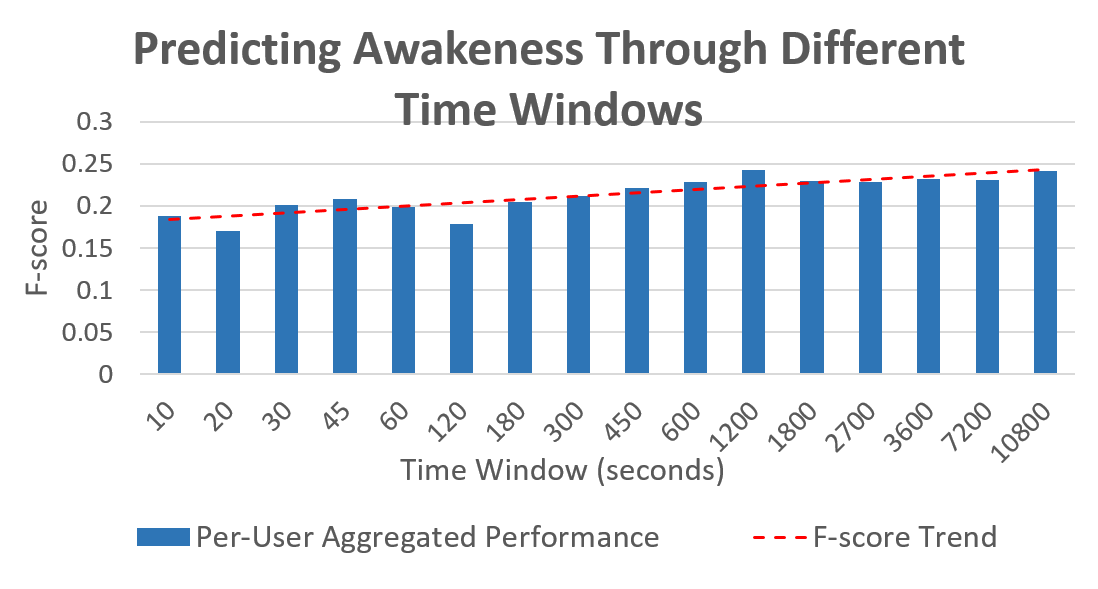
\includegraphics[width=0.5\textwidth]{20180912AwakenessTWBars.png}
  \caption{Performance (F-score) of individual classifiers trained on the different time windows to predict `awake'.}
  \label{timeWindowsPandR}
 % \vspace*{-3mm}
\end{figure}

%We also compared the performance of a model created per user against
%a model created across users.
%To calculate the performance of the model created per user,
%for each user we create a model using the features 
%related to each time window for the selected user only, 
%while in the model created with data across users,
%we trained the model with the data related to each
%particular time window of all users.
%our results show that the personalized model created
%for each user outperforms in every case
%the model created the with data across all users.

%This study
%shows that in general larger time windows predict stress,
%focus, and awakeness more precisely than 
%shorter time windows. We can also notice
%a very gentle upwards trend
%with a inflexion points at 45 seconds and 180.
%There is a peak of performance in 45 seconds, 
%time window that could be used if time is a scarce resource.
%The performance stabilizes around 180 time window
%which indicates that collecting data for a longer time
%period will not increase significantly the performance of the approach.
%The difference in performance between the 
%lowest performing and the highest performing time window is 
%less than a 10\% improvement. 


\subsection{Computer Interaction Data} \label{secCI}
Given our focus on knowledge workers (i.e., workers who generally spend a lot of time interacting with information on their computer at work), we also analyzed the use of computer interaction features to predict focus, awakeness and stress. To collect computer interaction data, we used an open source computer interaction monitor (reference omitted for double-blind.)
%the open source PersonalAnalytics project\footnote{https://github.com/sealuzh/PersonalAnalytics}  \cite{meyer18} 
to track participant's mouse and keyboard activity, as well as details about their active window. The specifics of the features tracked are listed in Table \ref{tracker}. The tracker was installed on the computers of 10 of the 14 participants, with participants S6, S10, S12, and S13 opting out of this part of the study due to privacy concerns.  Therefore, we limited this analysis to the 10 participants for whom we could calculate all features. 

\begin{table}
\begin{center}
\small\addtolength{\tabcolsep}{-1pt}
\begin{tabular}{l l}
\hline

Feature collected by tool & Description \\ 
\hline
Total keystrokes per min& Sum of all types of keystrokes \\ 
Normal keystrokes per min&F[h] Not backspace and navigation \\ 
Backspace keystrokes per min& Backspace keystrokes \\ 
Navigation keystrokes per min& Arrow key keystrokes \\ 
Total clicks per min& Sum of all click types \\ 
Other clicks per min& Not right and left clicks \\ 
Left clicks per min& Left clicks \\ 
Right clicks per min& Right clicks \\ 
Scrolled distance per min& Scrolled distance in pixels \\ 
Moved distance per min& Mouse movements in pixels \\ 
Activity switches per min& Browser window title changes \\ 
Category switches per min& Activity performed category \\ 
\hline
\end{tabular}
\caption{Features collected per user by the computer interaction tracker}%~\cite{meyer18}}
\label{tracker}
\end{center}
%\vspace*{-1mm}
\end{table}

For calculating computer interaction features, we again used the aforementioned 16 time windows and scaled the computer interaction values if the time windows did not align. For our comparative analysis of the different sensing techniques---biometrics vs computer interaction---we then created two new feature sets for each participant in addition to the biometric one: one with only computer interaction features, and one with computer interaction features plus biometric features. 

Table~\ref{ciPerformance} lists the results of our analysis. The results show that in all cases, the computer interaction based model was able to improve upon the biometric model in terms of precision and recall.
%MS is removing the accuracy results because it is not what we care about and it is just making the results harder to understand
%, but not in accuracy. 
Further, we found that the combined model was the most effective model in terms of precision and recall for predicting stress and awakeness overall, but performed slightly worse than the model using only computer interaction features for focus. 
%Since we consider precision and recall for predicting the class of higher interest, i.e. stressed, not focused, not awake, to be the most important statistics when interpreting our results, we compared the models against each other by averaging these two statistics.


\begin{table}
\begin{center}
%\small\addtolength{\tabcolsep}{-1pt}
\begin{tabular}{llllll}
\hline
Model/Feature Set & Precision & Recall & F-Score \\ %& Accuracy\\
\hline
\textbf{Awakeness}\\
\hspace{3mm}Biometrics only  & 0.269 & 0.314 & 0.289 \\ %& 0.808\\
\hspace{3mm}C.I. only  & 0.425 & 0.362 & 0.391 \\ % & 0.758\\
\hspace{3mm}Biometrics + C.I. & 0.390 & 0.404 & 0.400 \\ % & 0.791 \\
\hline
\textbf{Stress}\\
\hspace{3mm}Biometrics only  & 0.270 &	0.260 & 0.265 \\ % & 0.775\\
\hspace{3mm}C.I. only & 0.290 & 0.272 & 0.281 \\ % & 0.698 \\
\hspace{3mm}Biometrics + C.I. & 0.317 & 0.286 & 0.301 \\ % & 0.712\\
\hline
\textbf{Focus}\\
\hspace{3mm}Biometrics only & 0.251 & 0.256 & 0.253 \\ % & 0.716\\
\hspace{3mm}C.I. only & 0.332 & 0.342 & 0.337 \\ % & 0.742\\
\hspace{3mm}Biometrics + C.I. & 0.340 & 0.316 & 0.328 \\ % & 0.745\\
\hline
\end{tabular}
\caption{Comparison of the performance of predicting stress, focus and awakeness using the 3 different feature sets for the 10 participants. The performance is calculated as the average of the performance of the individual classifiers. Computer Interactions is abbreviated as C.I. here for readability. Precision and recall refer to the prediction of the more important classes, i.e. `stressed', `not awake', `not focused'.}
\label{ciPerformance}
\end{center}
%\vspace*{-1mm}
\end{table}

As with the biometric models, the individual performance of both the computer interaction only models and the combined models varied quite a bit between participants. Using stress as an example again, in the computer interaction models 5 of the 10 participants saw improvements compared to the baseline, with a maximum improvement of 128\% in precision, and 78\% in recall. In the combined model for stress, 5 of the 10 participants saw improvements compared to the baseline, with a maximum improvement of 117\% in precision and 95\% in recall. Neither model was capable of correctly predicting any instances of 'stressed' for participant S7.

Since the number of features changes  depending on which feature set is used, we adjusted the feature selection parameter for each of the computer interaction and combined computer interaction/biometric models. The values reported in this section were achieved using the optimal feature selection parameters we found, which are shown in Table \ref{ciFeatureSelection}.

\begin{table}
\begin{center}
\begin{tabular}{lc}
\hline
Model/Feature Set & Number of Features Selected\\
\hline
\textbf{Stress}\\
\hspace{3mm}C.I. & 400\\
\hspace{3mm}Biometrics + C.I. & 800\\
\hline
\textbf{Focus}\\
\hspace{3mm}C.I. & 20\\
\hspace{3mm}Biometrics + C.I. & 300\\
\hline
\textbf{Awakeness}\\
\hspace{3mm}C.I. & All\\
\hspace{3mm}Biometrics + C.I. & 50\\
\hline
\end{tabular}
\caption{The optimal number of features we found to select for each of the model/feature set combinations. Computer interactions is abbreviated as C.I.}
\label{ciFeatureSelection}
\end{center}
\vspace*{-4mm}
\end{table}


%!TEX root = bioPrediction_main.tex
\section{Discussion}
%\vspace{0.05in}
\noindent
\textbf{Implications for HCI Design and Workspaces:}
The results discussed in this paper establish great potential
to increase the well-being of knowledge workers and the quality of their work
through monitoring their biometric signals and computer interactions with the
goal of recognizing their stress, awakeness, and focus levels in an uninvasive 
and automatic manner. Being able to accurately recognize periods of high-
stress in workers enables companies to prevent or de-escalate potentially 
dangerous situations in the workplace, e.g. confrontation between co-workers. Similarly, this can help to design more team-based approaches such as an 
awareness dashboard of a team's stress level, and avoid digital interruptions in high-stress or high-focus periods similar to previous studies~\cite{zuger2017reducing}.
Likewise, awakeness and focus
can be enhanced given such a technology
through individual approaches such as adapting the lighting in a control 
room, or scheduling breaks to prevent focus loss.

Currently, the cost of biometric sensors and necessary infrastructure, such as automated light and sound systems for adjusting the environment, makes our approach most appropriate for high-value workspaces, such as control rooms, command centers, or dispatch offices. However, as standard office settings become more personalizable (e.g., via adjustable desks, lighting, and sound showers) and sensor costs decrease, our approach could be applied to any office environment, and thus could impact a large percentage of modern workers. As in modern cars, temperature and lighting could be regulated on a per-person basis, which would allow the environment to react to the person's current state and to maximize each person's preferences and productivity (e.g., preferences of men and women in temperature~\cite{Karjalainen07}). Further research would be needed to identify how to balance needs across a group of office workers and how to handle conflicting levels between different group members.

%\vspace{0.05in}
\noindent
\textbf{Imbalanced Data:}
Study participants provided highly imbalanced data in their survey responses, with most participants only taking advantage of a subset of the Likert-scale values and the data points mostly being clustered around the middle of the scale, as can be seen in Table~\ref{responseDistribution}. While some of the imbalance is expected due to certain classes, such as 'not stressed', being more common in the workplace, this imbalance also provides challenges in the training and assessment of a machine learning classifier, as also found by others, e.g.~\cite{Exler16}. We addressed this for the training by oversampling in case of few data samples for the individual models and undersampling in case of a general model where more data was available. Especially in light of this imbalance in the data, the results we achieved with our models are encouraging. For the assessment of the classifiers' performance we addressed the imbalance by not just presenting accuracy, but also by focusing on prediction and recall to examine the classifier's performance in predicting the infrequent (yet more important) cases, such as when a user is struggling to stay awake and an intervention or warning might be needed most. 
% \textbf{Unbalanced Data:}
% As shown in Table~\ref{responseDistribution}, the typical participant provided highly unbalanced survey responses, with most responses exhibiting a central tendency. Many participants provided zero or one very high (or very low) value on the Likert scale. In spite of this, our results show that by using biometric sensors and leveraging a machine learning approach, we are able to predict stress, focus, and awakeness better than the baseline, with improvements up to 84.64\%. Taking into account that the model correctly predicts many cases that happen infrequently, this is especially promising. These infrequent cases, such as when a user is highly stressed or struggling to stay awake, are in fact the most important cases to detect, as they are when intervention is needed most.

%\vspace{0.05in}
\noindent
\textbf{Ground Truth and Self-Reporting:} 
One of the key points for developing a good classifier for awakeness, focus and stress, is to collect a valid ground truth to be used as the output measure. When designing the study, we therefore spent an extensive amount of time on determining the exact questions to ask in the experience sampling, consulting experts in the area, and basing the questions and wording on previous research and studies. Yet, the reliability and validity of self-reports have been questioned in the past due to subjective biases, lack of care in reporting, and the highly individual nature of reporting aspects such as stress~\cite{Hernandez11,Hovsepian15}. In addition, in contexts such as the workplace, employees might be afraid to genuinely report levels of aspects, such as sleepiness. Hence, there is a chance that the collected experience samples do not adequately reflect the ground truth of the underlying variable under investigation. It could even be the case that certain biometrics might represent a more accurate ground truth of the studied phenomena than the self-reports. This suggests that a more confirmative study rather than an inquiry study could be a better approach, and we will explore such routes in future work.


%\vspace{0.05in}
\noindent
\textbf{Corpus Size:}
In this study we collected data from 14 professionals over the course of eight weeks. By scholarly standards this constitutes a large dataset --- especially given that the participants were not students. However, in the context of machine learning this corpus is relatively small. Thus, the model's overall performance, while promising, is only an indication of the performance that a larger corpus could provide. Our results show that there is a positive correlation between data added to the training corpus and the performance level of the model. This upwards trend likely continues, but a larger dataset is needed to confirm or reject this hypothesis. 

% \vspace{0.05in}
% \noindent
% \textbf{Data Collection:} 
% One advantage of our study is that it was conducted on professionals in a real office setting (i.e., not on students). However, the disadvantage to working with professionals is that business deadlines and other pressing real world issues lead to missing survey responses. Additionally, busy professionals often fall into the trap of always selecting the same value for a given question that they have answered many times, which reduces the accuracy of the collected data. To minimize the effect of this inertia, we advise collecting data at typical low-productivity times, such as in the early afternoon or on Mondays~\cite{mark2014bored}.

%\vspace{0.05in}
\noindent
\textbf{Per-User Model vs. Across-Users Model:}
Our results show that individually trained models outperform on average a more general model. Yet, given the increase in model performance with training data set size, we expect that with enough data, a generic model will perform reasonably close to the individually trained models. This would have significant practical implications, eliminating the need for survey-based feedback (which is only necessary for model training), and thereby completely automating measurement of human aspects. Our follow up work will focus on gathering more data toward this end.


% \vspace{0.05in}
% \noindent
% \textbf{Per-User Model vs. Across-Users Model:}\
% While we do see variations across participants, and thus our work shows that personal 
% models perform better than generic models, we expect that with enough data, a generic 
% model may perform equally well. This would have significant practical implications, eliminating the need for survey-based feedback (which is only necessary for model training), thereby completely automating measurement of human aspects. Our follow up work will focus on gathering more data toward this end and on evaluating the performance of a generic model.



%!TEX root = bioPrediction_main.tex
\section{Threats to Validity}
There are numerous threats to validity to our study.

\subsection{External Validity}
The results of our study may 
 not generalize to a broader population of office workers.
To mitigate this risk, we collected participants
from a wide variety of different departments
with different age ranges, genders, work experience, and 
working in different positions.

Another threat is that our results may not generalize
to a different office environment. We conducted
this study in a typical office environment, similar to many
among technology workers across the world.
These office environments control for a series of
variables to make them standard worldwide such
as controlled temperature and lighting.

\subsection{Internal Validity}
This study tries to find correlations between
biometric features and the human aspects of stress, focus, and awakeness.
Nonetheless, biometric signals are influenced by far more
variables than the ones this study comprehends.
Therefore, trying to draw a strong causality between the biometric
features and the aspects would be inaccurate.
To mitigate this risk,  we collected the data
in a rote environment and in a regular manner 
to minimize the number of 
external causes that may affect each participant's
biometric signals.

It is possible that the amount of data collected
is not sufficient
to draw valid conclusions. To address this threat, 
we collected a data for an eight-week period, which is
400\% longer than the longest previous studies~\cite{zuger18,Muller16}.

Due to the small amount of data available to us for the purposes of this study, there is a risk
that our models may be overfitting to some degree. Such overfitting indicates that the results presented in our work may be less than optimal, however any overfitting applies strictly to the training data and given that there is no overlap between the data used for training and testing, we do not believe this invalidates our results.
We leave further optimization of our approach to future researchers.


\subsection{Construct Validity}
A threat to the study is that
there are other factors that might either influence the
human aspects of interest or that were considered but
are unrelated biometric signals.
To mitigate this risk, we used a state-of-the-art
device that captures a large number of highly accurate biometric
signals. We collected the most commonly analyzed
biometrics that historically have shown correlation with 
the studied human aspects of stress, focus and awakeness.
In an effort to maintain this research applicable to real-world environments, we picked the already existing Everion device, even when, as a trade-off, we could not capture more descriptive and more intrusive signals such as SDNN, SCL, SCR, eye tracking, or brain activity.

A future more thorough statistical analysis of the relationships between
the aspects of interest, such as stress, and the physiological
data may further provide deeper insights into the data and
how it might be used in prediction.












%!TEX root = bioPrediction_main.tex
\section{Conclusions} 
Stress, awakeness and focus at work are highly relevant aspects when
it comes to productivity and well-being at the workplace. In this
paper, we presented the results of a study with 14 professional
knowledge workers in their workplace over an eight week period to
better understand how workers experience stress over time and to
examine the ability of biometrics to predict these
productivity-related aspects. The longitudinal and in situ placement of
the study support and extend previous work. Based on
twice collected daily survey responses, we observed that
although participants sometimes saw periods of sustained stress,
they would always return to a baseline stress level for them
at some point. We also observed that stress levels seldom spiked,
but when they did rise, the rise in stress tended to last more
than a day. In addition to the survey responses, we 
continually collected
biometrics data with which we were able to create a model that was able to
predict awakeness, stress, and focus.

These results open up new opportunities to help increase knowledge
workers' productivity and well-being, ranging from instantaneously
taking action to prevent potentially risky situations and prevent
accidents due to a lack of focus or awakeness, all the way to
recommending interventions to reduce stress if it becomes more
chronic.

% \todo{as you can see, the conclusion is way too long and has some cut and paste repetition}

% Stress, awakeness and focus at work are highly relevant aspects when it comes to productivity and well-being at the workplace. In this paper, we presented the results of a study with 14 professional knowledge workers in their workplace over an eight week period to examine the ability of biometrics for predicting these producitivity-related aspects. The longitude and in situ placement of the study as well as the breadth of human aspects examined, support and extend previous work. Based on twice collected daily survey responses and continually collected biometrics data we were able to create a model that was able to predict , outperforming the baseline by as much as 84.6\%, in the case of awakeness. We also show that there is a positive correlation between number of training instances and model performance--a 114\% improvement from training with one sample to training with 33 samples--suggesting that with a larger amount of training data prediction would continue to improve. Due to this, while current user-specific models have higher performance than across-user models, there is hope that with enough data even across-user models could become accurate. 


% Our analysis shows that we are able to \todo{fill this}

% Our study with 14 professional knowledge workers in their workplaces over an eight week period has shown that we can use biometrics to predict these producitivity-related aspects of an individual knowledge worker. The longitude and in situ placement of the study as well as the set of human aspects examined support and extend previous work. In addition, our analysis 

% as well as computer interaction features to predict these aspects of an individual knowledge worker
% has shown that we can use biometrics as well as computer interaction features to predict these aspects of an individual knowledge worker over a long period of time in situ
% The results also show that the general ... \todo{fill this}

% In this study we analyze biometric signals of office workers to predict the productivity-related human aspects of stress, focus, and awakeness. A key component of this study was its length, an eight week period, longer than previous studies by a factor of four~\cite{zuger18,Muller16}, and its realism , studying professionals in situ instead of students. We collected information from 14 participants from different departments within the company, covering different ages ranges, genders, and work experience. By learning from twice daily survey responses and continually collected biometrics data we were able to create a model that was able to predict human aspect values, outperforming the baseline by as much as 84.6\%, in the case of awakeness. We also show that there is a positive correlation between number of training instances and model performance--a 114\% improvement from training with one sample to training with 33 samples--suggesting that with a larger amount of training data prediction would continue to improve. Due to this, while current user-specific models have higher performance than across-user models, there is hope that with enough data even across-user models could become accurate. 

% From these results emerge a series of opportunities to help increase awakeness, focus, and reduce stress in office workers. In the near future, we will therefore be able to detect a decrease in productivity-related aspects following our approach, and be able to take action to prevent potentially risky situations.

%\begin{acks}
%The acknowledgments section will be included for the camera-ready version of the paper.
%\end{acks}



%\input{samplebody-conf}

% Balancing columns in a ref list is a bit of a pain because you
% either use a hack like flushend or balance, or manually insert
% a column break.  http://www.tex.ac.uk/cgi-bin/texfaq2html?label=balance
% multicols doesn't work because we're already in two-column mode,
% and flushend isn't awesome, so I choose balance.  See this
% for more info: http://cs.brown.edu/system/software/latex/doc/balance.pdf
%
% Note that in a perfect world balance wants to be in the first
% column of the last page.
%
% If balance doesn't work for you, you can remove that and
% hard-code a column break into the bbl file right before you
% submit:
%
% http://stackoverflow.com/questions/2149854/how-to-manually-equalize-columns-
% in-an-ieee-paper-if-using-bibtex
%
% Or, just remove \balance and give up on balancing the last page.
%
%\balance{}

%\bibliographystyle{ACM-Reference-Format}
%\bibliography{bp_bibliography}

%\end{document}


% BALANCE COLUMNS
\balance{}

% REFERENCES FORMAT
% References must be the same font size as other body text.
\bibliographystyle{SIGCHI-Reference-Format}
\bibliography{bp_bibliography}

\end{document}

%%% Local Variables:
%%% mode: latex
%%% TeX-master: t
%%% End:
